\documentclass[11pt]{article}
\usepackage[margin=1in]{geometry}
\usepackage[T1]{fontenc}
\usepackage[utf8]{inputenc}
\usepackage{lmodern,microtype}
\usepackage{amsmath,amssymb,amsthm,mathtools}
\usepackage{graphicx,booktabs,array,enumitem,setspace,placeins,longtable}
\usepackage{algorithm}
\usepackage{algpseudocode}
\usepackage{needspace}
\usepackage[authoryear,round]{natbib}
\usepackage[colorlinks=true,allcolors=blue]{hyperref}
\usepackage{bookmark}
\allowdisplaybreaks
\setstretch{1.18}
\setlength{\parskip}{0pt}
\setlength{\emergencystretch}{2em}
\setlist{itemsep=2pt,topsep=4pt}
\newtheorem{theorem}{Theorem}[section]
\newtheorem{lemma}[theorem]{Lemma}
\newtheorem{proposition}[theorem]{Proposition}
\newtheorem{corollary}[theorem]{Corollary}
\newtheorem{definition}[theorem]{Definition}
\newtheorem{example}[theorem]{Example}
\theoremstyle{remark}
\newtheorem{remark}[theorem]{Remark}
\newcommand{\E}{\mathbb E}
\newcommand{\Prob}{\mathbb P}
\newcommand{\ind}{\mathbf 1}
\newcommand{\kl}{\operatorname{kl}}
\newcommand{\pos}[1]{\left[#1\right]_+}
\newcommand{\suppproof}{Complete proofs appear in the supplementary material.}

% Set \anonymoustrue for an author-free review copy if required by the portal.
\newif\ifanonymous
\anonymousfalse
\title{The Cost of Reliable Near-Optimal Set Maintenance\\with Arriving Arms}
\ifanonymous
\author{}
\else
\author{Deqi Zheng\thanks{The first two authors contributed equally.} \quad
 Xiaoyang Xu\footnotemark[1] \\ Qiuzhen College, Tsinghua University
 \and Yuhong Yang\thanks{Corresponding author: yyangsc@mail.tsinghua.edu.cn.}\\
 Yau Mathematical Sciences Center, Tsinghua University}
\fi
\date{October 15, 2026}
\ifanonymous
\hypersetup{pdftitle={The Cost of Reliable Near-Optimal Set Maintenance with Arriving Arms},pdfauthor={}}
\else
\hypersetup{pdftitle={The Cost of Reliable Near-Optimal Set Maintenance with Arriving Arms},pdfauthor={Deqi Zheng, Xiaoyang Xu, Yuhong Yang}}
\fi
\begin{document}
\maketitle
\addtocontents{toc}{\protect\setcounter{tocdepth}{-1}}

\begin{abstract}
We study reliable maintenance of all relatively near-optimal arms while
collecting rewards when new arms arrive exogenously and remain available.
Reward laws are stationary, but arrivals change the membership boundary.
Reporting progress is measured by cumulative unresolved arm time outside
a prescribed boundary band, with simultaneous correctness of all labels.
One uncertain arrival can obstruct many earlier certifications. A
common-reference lower bound quantifies this effect, and matching
worst-schedule area bounds yield an arrival-growth boundary for joint
sublinear performance. On specified repeated-update families, temporary
membership tasks impose rapid-maintenance regret costs, while separate
constructions attain deferred and intermediate service levels. We develop
Flexible Certificate-Cost Planning (F-CCP) as a tunable implementation. It
combines sequential evidence and local certificate planning with a chosen
reward kernel and separate observable budgets for reward and
certification. Its guarantees include label reliability, unconditional
expected-regret protection, and service-rate area bounds that retain
budget rejections. Fixed-checkpoint and activation-budgeted constructions
remain distinct analytical witnesses. Frozen paired experiments show
lower mean costs in many finite-budget comparisons, together with
exceptions, heavier regret tails, and nonzero reporting failures. These
results do not characterize a general regret--maintenance frontier.
\end{abstract}
\noindent\textit{Keywords:} sequential experimentation; arriving arms;
near-optimal set maintenance; dynamic regret; confidence sequences.

\section{Introduction}
\label{sec:introduction}

Sequential experiments often acquire new candidates while earlier ones remain
available. An allocation rule must learn which candidates yield high rewards.
An experimenter may also need to know which of all available candidates are
within a specified tolerance of the current best. These objectives need not
favor the same observations. A candidate can be sufficiently inferior to
receive little reward-driven exploration and still be difficult to classify
relative to the near-optimality boundary.

We study these objectives together under permanent exogenous arrivals and
stationary reward laws. If $r^*(t)$ is the largest mean among the arms
available at time $t$, an arm is relatively near-optimal when its mean is at
least $r^*(t)-\varepsilon$. Reports certify membership, certify exclusion, or
leave the arm unresolved. We require one simultaneous correctness event for
all labels at all times. To rule out indefinite abstention, we charge the
cumulative unresolved time of arms whose means lie more than $\eta$ from
the membership boundary. The question is how much regret is necessary, and
how much is attainable, under this reporting requirement.

New arrivals affect the task in two ways. An uncertain new candidate may be
better than the incumbent by enough to invalidate many existing positive
reports. Evidence about that one candidate is then relevant to many
reports at once. A later improvement can also make an earlier difficult
membership question unnecessary: a candidate close to the old boundary may
be far below the new one. Its existing upper confidence bound can be
combined with a new reference's lower bound to certify exclusion. Neither
effect requires the reward law of an old arm to change.

Our observation model and regret comparator have established precedents.
Permanent arrivals form a monotone special case of sleeping-bandit
availability \citep{kleinberg2010}; ballooning bandits already compare reward
with the best arm currently available \citep{ghalme2021}. Exogenous arrivals
differ from drawing arms on demand from a reservoir
\citep{10.1214/aos/1069362389} and from the disappearing actions of mortal
bandits \citep{NIPS2008_788d9869}. Benchmark improvements here arise from new
arms, whereas nonstationary bandits allow the reward distributions of
existing arms to change \citep{Besbes2014,Auer2019ADSWITCH}. Sequential
allocation and adaptive experimentation have a long statistical history
\citep{Robbins1952,LAI19854,Lai1987}; the expanding set of actions retains
that allocation problem and adds an evolving inferential target.

For a fixed arm set, identifying every relatively near-optimal arm is the
ALL-$\varepsilon$ problem \citep{mason2020}. Joint reward and identification
objectives also have established precedents
\citep{degenne2019,yang2026,cho2025}. Our task requires continuing reports
under arrivals, with all-time label reliability and an explicit cumulative
cost for unresolved arm time. The distinction concerns the reporting
protocol and its cost, rather than a new arriving-arm model. The simultaneous
recovery scales used in our lower bounds build on existing information
inequalities and multiple-recovery arguments
\citep{kaufmann2016,malloy2014,jamieson2018}.

We give three results about maintenance cost. First, a common-reference
lower bound shows how one uncertain arrival can obstruct many other
certifications. Its information queue accumulates cost over time within
one reward environment. Second, we obtain matching worst-schedule orders
for cumulative unresolved area, including finite-horizon truncation, and
derive the polynomial arrival boundary for jointly sublinear area and
expected regret. This worst-case lower bound already occurs in an initial
static batch; the common-reference result describes a separate consequence
of continuing arrivals. Third, on a specified repeated-update family,
rapid resolution of temporary membership tasks has matching inverse-square
regret costs. Allowing a constant-factor larger area budget admits a
logarithmic regret upper bound. A nonvanishing-probability lower bound
holds in one fixed environment under the same cumulative-area requirement.
The deferred endpoint has only an upper bound. A separate activation-budgeted
witness covers an intermediate interval on a more strongly separated family;
the general causal frontier under overlapping arrivals remains open.


Fixed checkpoints make attainable costs explicit, but their quotas can
consume a moderate budget before useful reports appear. F-CCP uses every
observation to update valid reporting evidence and plans one certificate
observation at a time. A predictable priority controls the proposed
service rate. Separate budgets limit the virtual-index cost of reward
choices and of certification, so exploration by the reward kernel does
not exhaust the certification account. The resulting guarantees concern
reliability, regret protection, and conditional service bounds; the
local planning proxy is not a solution of the full statistical
allocation problem. The fixed-checkpoint witnesses are retained for
their original guarantees in the supplement.

The components have precedents. Betting processes provide time-uniform
inference for bounded means \citep{waudbysmith2024betting}; our particular
mixture and its bounded-reward validity are proved explicitly.
Thompson sampling supplies a flexible reward rule \citep{thompson1933}.
MOTS obtains fixed-arm minimax guarantees by modifying sampled scores
\citep{jin2021mots}. Our protection instead constrains the virtual-index
cost of the actual selected action under arrivals, and does not transfer
MOTS's theorem to a cold-temperature Beta rule. Conservative bandits
control performance against a fixed baseline \citep{wu2016conservative};
the two accounts here control index deficits and are not realized
shortfalls from a separately run baseline. The spectral accounting and
MC-MOSS concentration tools are inputs from the companion work
\citep{temporalgeometry2026}, not a new characterization claimed here.

Information about future task expiration also matters. A schedule-specific
comparator can defer a temporary question in a way that one causal policy
facing an unknown schedule cannot reproduce uniformly. We retain that
information distinction and an activation-budgeted intermediate-regime
result alongside the general maintenance bounds. The latter uses its own
window conditions and is not an optimality claim for F-CCP.

Section~\ref{sec:model} fixes the joint task and separates task parameters
from allocation preferences. Section~\ref{sec:method} presents F-CCP and
its guarantees. Sections~\ref{sec:maintenance} and~\ref{sec:tradeoff}
give the general costs, temporary-task bounds, and information limits.
Section~\ref{sec:experiments} evaluates frozen configurations, including
mean improvements, tail costs, failed reports, and the corrected
same-controller comparison.
\section{Model, reliable reports, and maintenance cost}
\label{sec:model}
\label{sec:problem}

\subsection{Observation model and regret}

Let $\mathcal A$ be a possibly infinite set of arms. Arm $i$ arrives at
time $\tau_i$, after which it remains available. At every physical time
$t=1,2,\ldots$,
\[
 \mathcal A_t=\{i:\tau_i\le t\},\qquad
 1\le K_t=|\mathcal A_t|<\infty.
\]
Arbitrary finite batches are allowed, including $K_T>T$ at an evaluation
endpoint. Each arm has an unknown stationary reward law on $[0,1]$ with
mean $r_i$. Its successive potential observations $(Y_{i,n})_{n\ge1}$ are
independent and identically distributed, and the streams of different arms
are independent. Arrivals are exogenous and independent of both these
streams and policy randomization. Unless stated otherwise, each result
is for a fixed deterministic arrival schedule.

At time $t$, the policy first receives all current arrivals, then selects
one arm $I_t\in\mathcal A_t$, observes one reward $X_{t,I_t}$, and finally
issues its report. It uses the observed history
\[
 H_{t-1}=(\mathcal A_s,I_s,X_{s,I_s})_{s=1}^{t-1}
\]
and independent randomization. Means, future arrivals, and true membership
labels are unavailable to the policy. With
$N_i(t)=\sum_{s\le t}\ind\{I_s=i\}$, the physical observation is
$X_{t,I_t}=Y_{I_t,N_{I_t}(t-1)+1}$. Write
\[
 \hat r_i(n)=\frac1n\sum_{s=1}^nY_{i,s},\qquad
 r^*(t)=\max_{i\in\mathcal A_t}r_i,\qquad
 \Delta_i(t)=r^*(t)-r_i \quad(i\in\mathcal A_t).
\]
At a deterministic endpoint $T$, cumulative dynamic regret is
\[
 R_T(\pi)=\sum_{t=1}^{T}\Delta_{I_t}(t).
\]
This is a sum of mean gaps, random through the policy's arm selections;
$\E R_T$ is its expectation. The quantity does not compare realized
reward sequences. Physical time always counts actual observations.

\subsection{Reliable reports and cumulative unresolved time}
\label{sec:reporting_task}

For $0<\varepsilon<1$, the target set is
\[
 \mathcal G_t^\varepsilon=\{i\in\mathcal A_t:\Delta_i(t)\le\varepsilon\}.
\]
After the current observation, a report partitions all of $\mathcal A_t$
into $\mathcal P_t,\mathcal N_t,\mathcal V_t$: certified members, certified
nonmembers, and unresolved arms. Define
\[
 E_{\rm lab}=\{\text{for all }t:\ \mathcal P_t\subseteq\mathcal G_t^\varepsilon
                  \subseteq\mathcal A_t\setminus\mathcal N_t\}.
\]
A policy is $\delta$-reliable if $\Prob(E_{\rm lab})\ge1-\delta$ in every
allowed reward environment. A positive report may be withdrawn after a new
arrival. On the correctness event, a negative report remains valid because
$r^*(t)$ is nondecreasing and the arm's mean is stationary.

Reliability permits all arms to remain unresolved. For a boundary width
$0<\eta<1$, define
\begin{equation}
 \begin{split}
 d_i^\varepsilon(t)&=|\Delta_i(t)-\varepsilon|,\\
 U_t(\eta)&=\sum_{i\in\mathcal A_t}
   \ind\{i\in\mathcal V_t,d_i^\varepsilon(t)>\eta\},\qquad
 \mathcal U_T(\eta)=\sum_{t=1}^{T}U_t(\eta).
 \end{split}
 \label{eq:area}
\end{equation}
The count includes newly arrived arms with no observations and old arms
that become unresolved again. Every such arm--time pair is charged; the
loss is not limited to the time before a first decision. Within the
boundary band, unresolved time is exempt, but any label issued there must
still be correct. The true distance $d_i^\varepsilon(t)$ is used only by
the evaluator and in the analysis.

Task parameters are fixed within a comparison. Allocation preferences
change the strategy, rather than the reporting target. The parameters
used below have the following roles.
\begin{center}
\small
\begin{tabular}{lp{.67\textwidth}}
\toprule
Parameter & Role\\
\midrule
$\varepsilon,\eta\in(0,1)$ & Membership tolerance and exempt boundary width\\
$\delta\in(0,1/2)$ & Simultaneous reporting error budget\\
$\lambda_t\in[0,1]$ & Predictable preference for certification\\
$p_0\in(0,1),\ k_0>0,\ \nu>0$ & Service floor, backlog scale, and planning price floor\\
$\mathsf B,\ \theta>0$ & Reward-score kernel and its temperature\\
$\beta_R,\beta_C\in[0,\infty]$ & Fixed reward and certification guard coefficients\\
$\rho$ & Auxiliary checkpoint precision; F-CCP uses $\eta/4$\\
\bottomrule
\end{tabular}
\end{center}
The fixed-checkpoint witnesses may prescribe other precisions before
observations. Preference switching does not change
$\varepsilon,\eta,\delta$, create observations, or reset accumulated
evidence or budget accounts.


The main requirement at a fixed $T$ is
\begin{equation}
 \E_\vartheta R_T\le r,\qquad
 \Prob_\vartheta\{E_{\rm lab},\mathcal U_T(\eta)\le a\}\ge1-\delta.
 \label{eq:joint_protocol}
\end{equation}
It combines an expected regret bound with a joint high-probability
label--area guarantee. In particular, $\mathcal U_T=o(T)$ requires the
time-average number of unresolved separated arms to vanish, rather than
only a small unresolved fraction of all arms. The area guarantee is for
each deterministic endpoint; it need not hold for every endpoint on one
common area event.

For a performance family $\Theta$, let $\mathfrak R_\Theta(a)$ be the
infimum of $\sup_{\vartheta\in\Theta}\E_\vartheta R_T$ over policies reliable on
the full bounded model and satisfying the probability condition in
\eqref{eq:joint_protocol} for every $\vartheta\in\Theta$. The value is
$+\infty$ if the feasible class is empty. Full-model label reliability
and a family-specific area guarantee are distinct requirements. The
lower bounds remain valid when reliability is required only on the
lower-bound subfamily.

\subsection{How arrivals change the reporting problem}

For a fixed old arm, $\Delta_i(t)$ is nondecreasing, so its true membership
can change only from member to nonmember. Its boundary distance
$|\Delta_i(t)-\varepsilon|$ need not be monotone. A new candidate can first
create uncertainty about the current best mean, obstructing positive
certification of many old arms even when those arms remain truly
near-optimal. A sufficiently good new reference can later move the
boundary past earlier candidates, making their fine classification
unnecessary. Sections~\ref{sec:maintenance} and~\ref{sec:tradeoff} quantify
these two effects under the same reporting protocol.


Arms with close means need not be close to the relative boundary
$r^*(t)-\varepsilon$. Conversely, a candidate near that boundary can
require fine evidence even when its reward gap is appreciable. The
algorithm's observable work set is therefore defined from confidence
intervals, not from the evaluator's true gaps or unresolved area.
\section{Flexible certificate-cost planning}\label{sec:fccp}\label{sec:method}
The reporting task need not receive a fixed fraction of every sampling
budget. Evidence obtained while collecting rewards can already certify
some arms, and a small amount of additional work can complete other
reports. Flexible Certificate-Cost Planning (F-CCP) uses one set of lifetime
statistics for both purposes. Its service preference controls how often
certification is attempted; two separate budgets protect the reward
allocation and reserve capacity for certification. The resulting guarantees
concern reliable labels, regret order, and service completion. They do not
identify the optimal allocation for every joint regret--area constraint.

\subsection{Evidence and current reporting work}\label{sec:fccp-evidence}
Order arms by arrival, with a fixed order within each batch. Write
$n_i=N_i(t-1)$ and $\Sigma_i$ for the actual count and reward sum available
before the action at time $t$. Initially $n_i=\Sigma_i=0$ and
$[\ell_i,u_i]=[0,1]$. For $\alpha_i=\delta/\{2i(i+1)\}$, invert the
beta-mixture process
\begin{equation}\label{eq:fccp-mixture}
 \mathsf M_{i,n}(m)=
 \frac{\operatorname B(\Sigma_{i,n}+1/2,n-\Sigma_{i,n}+1/2)}
 {\operatorname B(1/2,1/2)m^{\Sigma_{i,n}}(1-m)^{n-\Sigma_{i,n}}},
 \qquad m\in[0,1],
\end{equation}
where $\operatorname B$ is the beta function, distinguished from the
optimal mean $r^*(t)$. The interval is the intersection of
$\{m:\mathsf M_{i,n}(m)\le1/\alpha_i\}$ over all observed positive
prefixes. At the actual count
\begin{equation}\label{eq:fccp-quota}
 \rho=\eta/4,\qquad
 q_i=\left\lceil\frac{2}{\rho^2}
             \log\frac{4i(i+1)}{\delta}\right\rceil,
\end{equation}
intersect it also with
$[\hat r_i(q_i)-\rho/2,\hat r_i(q_i)+\rho/2]\cap[0,1]$.
Continue the mixture updates after this checkpoint. The construction is
valid for bounded rewards, including nonbinary rewards; its supermartingale
argument is given in Supplement~\ref{app:fccp-evidence}. Sequential betting
and mixture confidence sequences are established tools
\citep{waudbysmith2024betting}.

For a nonempty confidence rectangle define
\begin{equation}\label{eq:fccp-gap}
 g_i^-=\max\{0,\max_{j\ne i}\ell_j-u_i\},\qquad
 g_i^+=\max\{0,\max_{j\ne i}u_j-\ell_i\}.
\end{equation}
Both bounds are zero when there is only one arm. They are the exact
minimum and maximum of the gap over this rectangle, including its
self-exclusion constraint. After observing a reward, report
\begin{equation}\label{eq:fccp-report}
 \mathcal P_t=\{i:g_i^+\le\varepsilon\},\quad
 \mathcal N_t=\{i:g_i^->\varepsilon\},\quad
 \mathcal V_t=\mathcal A_t\setminus(\mathcal P_t\cup\mathcal N_t).
\end{equation}
A negative report does not remove an arm from future reward allocation.
Among unresolved arms let
\begin{equation}\label{eq:fccp-work}
 Z_t=\{i\in\mathcal V_t:[g_i^-,g_i^+]
                 \subseteq[\varepsilon-\eta,\varepsilon+\eta]\},
 \qquad W_t=\mathcal V_t\setminus Z_t.
\end{equation}
These formulas are also evaluated before the action, after the current
arrivals, when choosing that round's service. An arm in $Z_t$ remains
reported as unresolved; the rectangle already shows that it incurs no
$\eta$-unresolved cost. Recompute the sets after every arrival and
observation. An empty interval sets a persistent failure flag: all
subsequent reports are unresolved and designated service stops. Reward
allocation, its guard, and the actual statistics continue.

\subsection{A local certificate plan}\label{sec:fccp-plan}
The plan assigns observations a positive price and asks which current
pairwise certificate is cheapest to pursue. Its centers and radii are
\begin{equation}\label{eq:fccp-planning}
 m_i=\Pi_{[\ell_i,u_i]}\frac{\Sigma_i+1/2}{n_i+1},\quad
 v_i^{\mathrm{plan}}=\max(m_i-\ell_i,u_i-m_i),\quad
 \bar n_i=\max(1,n_i).
\end{equation}
Here $\bar n_i$ is a planning convention; no fictitious observation enters
the confidence interval. For each $i\in W_t$, take as its reference $j$
the arm of largest $m_j$ if $\max_km_k-m_i>\varepsilon$; otherwise take
the largest-upper-bound arm other than $i$. Resolve reference ties by arrival
order. Set
\begin{equation}\label{eq:fccp-price}
 h_i=.95\max\{|m_j-m_i-\varepsilon|,
                   \eta-|m_j-m_i-\varepsilon|\},\quad
 c_k=\nu+(1-\lambda_t)\zeta_t(k),\quad
 a_k=v_k^{\mathrm{plan}}\sqrt{\bar n_k},
\end{equation}
where $\nu>0$ and the observable index gap $\zeta_t$ is defined below.
Solve the two-coordinate proxy problem
\begin{equation}\label{eq:fccp-pair}
 \min_{x_i\ge\bar n_i,\,x_j\ge\bar n_j}
  c_i(x_i-\bar n_i)+c_j(x_j-\bar n_j)
 \quad\text{subject to}\quad
  a_i/\sqrt{x_i}+a_j/\sqrt{x_j}\le h_i.
\end{equation}
The interior solution is explicit; boundary and zero-radius cases appear
in Supplement~\ref{app:fccp-evidence}. Among pairs with an available
endpoint, use the pair of smallest proxy cost. Within that pair, select
the endpoint maximizing $v_k^{\mathrm{plan}}/(\bar n_kc_k)$ among those
with $n_k<q_k$ and $x_k>n_k$ (using the actual count). Execute only one pull,
then replan. If no pair provides an endpoint, select the widest interval
among arms with $n_k<q_k$, with arrival order breaking ties. Call this
subroutine $\operatorname{Plan}_t$, and its proposed arm $j_t$.

The optimization in \eqref{eq:fccp-pair} is exact for its continuous
proxy. It holds the centers fixed and approximates radius reduction by
an inverse square root. Other competitors can remain after one pair is
resolved. Thus its solution is a scheduling rule, not an information
complexity or a proof of optimal statistical allocation.

\subsection{Virtual indices and two budgets}\label{sec:fccp-budgets}
The reward guard uses a virtual, clipped MC-MOSS index. Its arrival clock
and spectral comparison come from the companion study
\citep{temporalgeometry2026}. Initialize $\mathrm{base}=0$. After arrivals,
if $K_t>1$ and either $\mathrm{base}=0$ or $K_t-1\ge2\,\mathrm{base}$,
set $\mathrm{base}=K_t-1$, $\sigma=t$, and
$d_{\mathrm{clock}}=2\,\mathrm{base}$. Retain all observations. With
$s=t-\sigma+1$, define
\begin{equation}\label{eq:fccp-index}
 J_i(t)=\begin{cases}
 1,&n_i=0,\\
 \min\{1,\hat r_i(n_i)+
       \sqrt{[\log\{s/(d_{\mathrm{clock}}n_i)\}]_+/n_i}\},&n_i>0,
 \end{cases}\qquad
 \zeta_t(i)=\max_jJ_j(t)-J_i(t).
\end{equation}
When $K_t=1$, set $J_i=1$ and $\zeta_t(i)=0$ without using an
uninitialized clock. The virtual index never forces an observation by
itself. In particular, $\zeta_t$ is an observable index difference,
not realized regret or a difference between two independent runs.

Choose the first initial arm as a counting anchor. Among all other
arrived arms, let $k_{\ell,t}$ count current ages $t-\tau_i+1$ in group
$0$ (age one), or group $\ell\ge1$ (ages in
$(2^{\ell-1},2^\ell]$). The current spectrum and its running maximum are
\begin{equation}\label{eq:fccp-spectrum}
 \mathcal S_t=\sum_{\ell\ge0}
       \min\{2^\ell,\sqrt{k_{\ell,t}2^\ell}\},\qquad
 \overline{\mathcal S}_t=\max_{u\le t}\mathcal S_u.
\end{equation}
The anchor's identity supplies no information about its mean or
optimality. Computing \eqref{eq:fccp-spectrum} uses only arrived arms'
current ages, with no endpoint or future-arrival input.

Fix $\beta_R,\beta_C\in[0,\infty]$ before the run. Maintain separate
ledgers, initially zero,
\begin{equation}\label{eq:fccp-ledgers}
 C_R(t)=\sum_{u\le t:\,\mathrm{reward}}\zeta_u(I_u),\qquad
 C_C(t)=\sum_{u\le t:\,\mathrm{service}}\zeta_u(I_u).
\end{equation}
Accept a proposed service only if
$C_C(t-1)+\zeta_t(j_t)\le\beta_C\overline{\mathcal S}_t$.
Otherwise use a reward round and record a denial. On any reward round
maximize the selected reward kernel's scores over
\begin{equation}\label{eq:fccp-feasible}
 \mathcal F_R(t)=\{i:C_R(t-1)+\zeta_t(i)
                                  \le\beta_R\overline{\mathcal S}_t\}.
\end{equation}
A largest-$J_i$ arm has zero index gap, so this set is nonempty. An infinite
budget disables the corresponding check, including when the spectrum is
zero; it is implemented as \texttt{None}, rather than as budget zero.
No ledger is reset at a clock change or preference change.

For example, the default reward scores are one draw per arm,
\begin{equation}\label{eq:fccp-score}
 \Xi_i(t)\sim\operatorname{Beta}
       (1+\Sigma_i/\theta,\,1+(n_i-\Sigma_i)/\theta).
\end{equation}
For Bernoulli rewards, $\theta=1$ gives standard Beta$(1,1)$ Thompson
sampling \citep{thompson1933}; $\theta=.5$ is a colder action rule.
For general bounded rewards these fractional-count scores are a
sampling heuristic. The evidence always uses the original counts and
reward sums. On a reward round draw the full score vector once, then
maximize that same vector over \eqref{eq:fccp-feasible}; do not redraw
following rejection. UCB1, Growing-MOSS, MC-MOSS, and KL-UCB can also
supply reward scores.

\subsection{Service preference and executable rule}\label{sec:fccp-modes}
Let $\lambda_t\in[0,1]$ be a predictable service preference. Given a
proposed service $j_t$, write $b_t=|W_t|$ and
$\widehat c_t=\max_i m_i-m_{j_t}$. The adaptive controller uses
\begin{equation}\label{eq:fccp-rate}
 w_t=p_0+(1-p_0)\frac{b_t}{b_t+k_0}
                         \frac{\varepsilon}{\varepsilon+\widehat c_t},
 \qquad
 p_t=\begin{cases}
 0,&b_t=0\text{ or service is disabled},\\
 \displaystyle\frac{\lambda_tw_t}{1-\lambda_t+\lambda_tw_t},&\text{otherwise}.
 \end{cases}
\end{equation}
Fixed-rate control instead uses $p_t=\lambda_t\ind\{b_t>0\}$.
Service is disabled when the failure flag is set or $\lambda_t=0$.
The presets use $p_0=.02$, $k_0=4$, and $\nu=.1$.
Few or costly proposed certificates tend to reduce the service rate;
a large, inexpensive backlog tends to increase it. The controller sees
$W_t$, not the true unresolved area. Neither $\lambda_t$ nor $w_t$ is
an estimated optimal multiplier or a forecast of future arrivals.

Use a phase $\phi_0=0$: add $p_t$ each round, and if the result is at
least one, attempt one service and subtract one. A denial does not
refund this phase. In exact arithmetic the number of attempts through
$T$ is $\lfloor\sum_{t\le T}p_t\rfloor$. For fixed $\lambda>0$,
on busy rounds,
\begin{equation}\label{eq:fccp-pmin}
 p_t\ge p_{\min}(\lambda):=
          \frac{\lambda p_0}{1-\lambda+\lambda p_0}>0.
\end{equation}
There is no positive service lower bound at $\lambda=0$.
Table~\ref{tab:fccp-modes} separates the four presets. Changing only
\texttt{set\_priority(1)} does not disable an existing certification
budget. Preference changes occur between completed physical rounds and
retain the phase, evidence, counts, and both ledgers.

\begin{table}[t]
\centering\small
\caption{F-CCP presets. The default reward kernel is Beta sampling.
An inactive service budget is never checked because service is off.
The guarantees refer to the conditions stated in this section.}
\label{tab:fccp-modes}
\begin{tabular}{lcccc}
\toprule
Preset (data ID)&$\lambda$/control&$\theta$&$\beta_R$&$\beta_C$\\
\midrule
Reward (F-R)&0/off&.5&16&inactive\\
Balanced (F-auto-0.6)&.6/adaptive&.5&16&1\\
Classification (F-area)&1/fixed&.5&16&$\infty$\\
Compatibility (F-R-TS-exact)&0/off&1&$\infty$&inactive\\
\bottomrule
\end{tabular}
\end{table}

\begin{algorithm}[tbp]
\caption{Flexible certificate-cost planning (F-CCP)}\label{alg:flexible-ccp}
\footnotesize
\begin{algorithmic}[1]
\Require Fixed $\varepsilon,\eta,\delta$, budgets $\beta_R,\beta_C$,
reward kernel, temperature, controller parameters; predictable $\lambda_t$.
\State Initialize empty arm statistics, intervals, and quotas;
$\mathrm{base}=0$, $\phi=C_R=C_C=\overline{\mathcal S}=0$; failure $=\mathrm{false}$.
\For{each physical time $t=1,2,\ldots$}
 \State Admit the current batch in arrival order with $n_i=\Sigma_i=0$,
 $[\ell_i,u_i]=[0,1]$, birth $t$, and quota \eqref{eq:fccp-quota}.
 \State Update the arrival clock and calculate $J_i(t),\zeta_t(i)$
 using \eqref{eq:fccp-index} (use the singleton convention).
 \State Update $\overline{\mathcal S}\gets
 \max\{\overline{\mathcal S},\mathcal S_t\}$ using current ages.
 \State Set attempt $=\mathrm{false}$, service $=\mathrm{false}$, $p_t=0$.
 \If{not failed and $\lambda_t>0$}
  \State Recompute the pre-action reports and $W_t$ from current intervals.
  \If{$W_t\ne\varnothing$}
   \State $j_t\gets\operatorname{Plan}_t$ using
   \eqref{eq:fccp-planning}--\eqref{eq:fccp-pair}; calculate $p_t$.
   \State $\phi\gets\phi+p_t$.
   \If{$\phi\ge1$}
    \State $\phi\gets\phi-1$; attempt $=\mathrm{true}$.
   \EndIf
  \EndIf
 \EndIf
 \If{attempt and a legal $j_t$ exists}
  \If{the service guard is off or
  $C_C+\zeta_t(j_t)\le\beta_C\overline{\mathcal S}$}
   \State $I_t\gets j_t$; service $=\mathrm{true}$;
   $C_C\gets C_C+\zeta_t(I_t)$.
  \Else
   \State Record one service denial; retain the decremented phase.
  \EndIf
 \EndIf
 \If{not service}
  \State Generate the reward score vector once from the current actual history.
  \State $I_t\gets$ first maximizer of these scores over $\mathcal F_R(t)$
  (all $\mathcal A_t$ when that guard is off).
  \State $C_R\gets C_R+\zeta_t(I_t)$.
 \EndIf
 \State Pull $I_t$ once; observe $X_{t,I_t}$;
 $n_{I_t}\gets n_{I_t}+1$, $\Sigma_{I_t}\gets\Sigma_{I_t}+X_{t,I_t}$.
 \If{not failed}
  \State Intersect the selected arm's interval with its new mixture interval;
  at $n_{I_t}=q_{I_t}$ also intersect the fixed-prefix interval.
  \State If any interval is empty, set failure $=\mathrm{true}$ permanently.
 \EndIf
 \State Report \eqref{eq:fccp-report}, or
 $(\varnothing,\varnothing,\mathcal A_t)$ if failed.
\EndFor
\end{algorithmic}
\end{algorithm}

Within a planned pair, equal endpoint scores favor the candidate $i$;
other ties use the fixed arrival-order scans. The procedure sees no
means, hidden identities, future arrivals, or endpoint. Stopping at an
arbitrary endpoint leaves the last completed report unchanged. Its
straightforward implementation takes $O(K_t^2)$ work per round when pair
planning or the self-excluding gap bounds are evaluated by nested scans,
and $O(K_t)$ stored arm statistics. Numerical root finding and floating
comparisons are described separately in the supplement.

\FloatBarrier
\subsection{Reliability, reward protection, and service completion}
\begin{proposition}[Reliable reports]\label{prop:fccp-report}
Under the bounded stationary model, every legal predictable choice of
preferences, prices, and service actions in F-CCP satisfies
$\Prob(E_{\mathrm{lab}})\ge1-\delta$. On a common event
$\mathcal E$ of this probability, all confidence intervals cover their
means at all observed counts, all reports are correct, and every arm in
$Z_t$ lies in the boundary band.
\end{proposition}
The evidence argument does not require the proxy plan to predict its
actual sampling cost. The mixture and checkpoint errors each receive
$\delta/2$, and a union bound gives $\mathcal E$.

\begin{proposition}[Compatibility endpoint]\label{prop:fccp-compat}
Fix a legal reward kernel $\mathsf B$. If service is off from the start
($\lambda_t\equiv0$), $\beta_R=\infty$, and the complete kernel state,
initialization, and random-number source agree with those of
$\mathsf B$, the two procedures have identical actions, lifetime counts,
and regret on every potential reward realization and arrival schedule.
\end{proposition}
This is a same-backend pathwise statement. A common seed in different
random-number backends does not provide the required coupling. The
colder, guarded F-R preset is distinct from this endpoint. Switching off
service after using it does not recreate a baseline's independent past.

The regret comparison uses an arbitrary-action inequality,
\begin{equation}\label{eq:fccp-optimism}
 \E R_T\le\min\left\{T,300\mathcal S_T+
                          \E\sum_{t\le T}\zeta_t(I_t)\right\}.
\end{equation}
Supplement~\ref{app:optimism-gap} proves the bridge from the companion
MC-MOSS potential-prefix and arrival-clock bounds to arbitrary actions;
the potential-prefix bounds apply to the actual sequence of selected actions.

\begin{theorem}[Two-budget reward protection]\label{thm:fccp-budget}
Fix finite nonnegative $\beta_R,\beta_C$ and use legal pre-observation
actions. For every deterministic schedule and endpoint,
\begin{equation}\label{eq:fccp-regret-finite}
 \E R_T\le\min\{T,(300+2\beta_R+2\beta_C)\mathcal S_T\}.
\end{equation}
If service is off throughout the run, omit $2\beta_C$ even when its guard is disabled.
If $\beta_R<\infty$ and $\beta_C=\infty$, then, with
$Q_T^{\mathrm{cap}}=\sum_{i\in\mathcal A_T}q_i$,
\begin{equation}\label{eq:fccp-regret-unlimited}
 \E R_T\le\min\{T,(300+2\beta_R)\mathcal S_T+Q_T^{\mathrm{cap}}\}.
\end{equation}
These bounds are unconditional, including reporting failures.
\end{theorem}
The ledgers satisfy their respective running-spectrum budgets, and
$\overline{\mathcal S}_T\le2\mathcal S_T$.
Substitution in \eqref{eq:fccp-optimism} proves the finite-budget bound.
Unlimited certification costs at most $Q_T^{\mathrm{cap}}$ actual
service pulls. Thus F-R has the conservative bound $332\mathcal S_T$,
Balanced has $334\mathcal S_T$, and Classification retains the extra
$Q_T^{\mathrm{cap}}$ term. The companion spectral minimax lower bound
makes the finite-budget regret order sharp, for fixed coefficients;
the spectral characterization itself is an existing input
\citep{temporalgeometry2026}. None of these bounds compares F-CCP's
realized regret with an independently run Thompson sampler.

\begin{theorem}[Area under a positive service rate]\label{thm:fccp-area}
Suppose every pre-action busy round has $p_t\ge p_{\min}>0$.
Let $D_T^{\mathrm{srv}}$ be the number of service attempts rejected by
the certification budget. On $\mathcal E$, simultaneously at every
endpoint,
\begin{equation}\label{eq:fccp-area}
 \mathcal U_T(\eta)\le K_T\min\left\{T,
                  \frac{Q_T^{\mathrm{cap}}+D_T^{\mathrm{srv}}+1}{p_{\min}}
                                      \right\}.
\end{equation}
When $D_T^{\mathrm{srv}}=0$, this is
$O(\min\{K_TT,K_T^2\eta^{-2}\log(K_T/\delta)/p_{\min}\})$.
\end{theorem}
Here busy means that the current $W_t$ is nonempty after arrivals and
before observation. If every current arm has reached its checkpoint,
the gap intervals are narrow enough that $W_t$ is empty. Each successful
service therefore advances a finite remaining checkpoint, and phase
accounting bounds the number of busy rounds. This proves the theorem
without requiring a cost-optimal plan. Classification has $p_{\min}=1$
and no refusals, hence the worst-area order matches the general lower
bound in its common parameter range. Finite-budget Balanced must retain
the denial term; it has no unconditional prescribed-area guarantee.
An arbitrary predictable $\lambda_t$ preserves label reliability, but
completion speed needs the displayed positive lower bound.

\begin{corollary}[Finite-arm completion]\label{cor:fccp-finite}
Suppose $\beta_C>0$ is fixed, busy rounds have a uniform positive service
rate, and arrivals eventually stop with finitely many arms. On
$\mathcal E$, every arm outside the boundary band eventually receives
a definite label. This conclusion holds regardless of continuing
reward-kernel exploration and its separate ledger consumption.
\end{corollary}
A conservative finite-prefix bound, the compatibility proof, and a
one-round obstruction to exact all-environment dominance appear in
Supplement~\ref{app:fccp-guarantees}. Completion on a fixed-confidence
event concerns the boundary band; it is not unconditional almost-sure
consistency for the exact oracle set.
\section{Fundamental costs of continual maintenance}
\label{sec:maintenance}

\subsection{One uncertain arrival can obstruct many reports}

The first lower bound retains one reward environment throughout the time axis.
It therefore measures a cumulative burden without adding the worst cases of
incompatible experiments. Fix
$0<\varepsilon\le1/16$, $0<\delta\le1/16$, and $0<\eta<\varepsilon/2$.
An initial reference has Bernoulli mean $1/4+\varepsilon/2$. Candidates arrive
on any prescribed schedule. In environment zero each has mean $p=1/4$;
environment $j$ changes only candidate $j$ to mean $p+2\varepsilon$.
All candidates are good in environment zero, with boundary distance
$\varepsilon/2$. After candidate $j$ arrives in environment $j$, every other
candidate is bad.

Let $M_t$ count arrived candidates and $a_t=M_t-M_{t-1}$. Define
\begin{align}
 q_-&=\left\lfloor\frac{\kl(1/4,\delta)}
                              {\kl(1/4,1/4+2\varepsilon)}\right\rfloor,
 &Q_t&=(Q_{t-1}+q_-a_t-1)_+,\quad Q_0=0,\notag\\
 \mathcal B_T&=\sum_{t\le T}(M_t-1)_+\ind\{Q_t>0\}.
 \label{eq:broadcast_queue}
\end{align}
This analytical queue is an information-capacity certificate: arrivals add
$q_-$ units per candidate, while only one observation is possible per round.
It is distinct from F-CCP's phased service rule and from the
fixed-checkpoint witness's FIFO queue. It imposes no pathwise sampling
quota on every candidate. In the stated
range $q_-\ge2$.

\begin{theorem}[Broadcast uncertainty]
\label{thm:broadcast}
For every policy reliable on environment zero and all its one-candidate
alternatives,
\[
 \E_0\mathcal U_T(\eta)\ge(3/4-\delta)\mathcal B_T.
\]
If $\mathcal B_T>0$, then
\[
 \Prob_0\{\mathcal U_T(\eta)\ge\mathcal B_T/4\}\ge1/4.
\]
These conclusions still hold when the policy knows the full arrival schedule,
the horizon, and the reference distribution.
\end{theorem}

At a busy time, some deterministic candidate label has expected sample count
below $q_-$. Changing that candidate alone has too little history KL to permit
positive certification of another candidate with probability at least $1/4$.
Reliability also bounds incorrect negative reports. The remaining probability
must be unresolved. The same reference environment supports this argument at
every time; the difficult label is selected from expected counts rather than
from a favorable realized history. The supplementary proof includes the
bounded-variable step needed for the probability statement.

If $m$ candidates have arrived by time $s$, the queue obeys the deterministic
inequality
\begin{equation}
 \sum_{t\le s+qm-1}(M_t-1)_+\ind\{Q_t(q)>0\}
                  \ge\frac{q-1}{2}m(m-1),\qquad q\ge2.
 \label{eq:queue_area}
\end{equation}
The factor $m^2$ reflects the number of affected reports as well as the work
needed to exclude high-quality alternatives. The subtraction of one unit in
$q-1$ accounts for the last observation of each busy period: reports are issued
after service.

\subsection{Worst-schedule maintenance area}

Let $\mathfrak A_{T,K}$ be the smallest $a$ attainable by a full-model reliable
policy with
\[
 \sup_{\boldsymbol\tau:K_T\le K}\sup_{\boldsymbol r}
 \Prob_{\boldsymbol r}\{E_{\rm lab}^c\ \text{or}\ \mathcal U_T(\eta)>a\}\le\delta.
\]
This optimization imposes no regret budget. Policies may know $T,K$ and the
schedule for the lower bound. The upper bound uses neither $T$ nor $K$ as
input.

\begin{theorem}[Worst-schedule area and joint attainability]
\label{thm:worst_area}
For integers $K\ge2$ and $T\ge1$, $0<\varepsilon\le1/8$,
$0<\eta\le\varepsilon/32$, and $0<\delta\le1/16$,
\begin{equation}
 2^{-24}\min\left\{KT,\frac{K^2}{\eta^2}\log\frac K\delta\right\}
 \le\mathfrak A_{T,K}\le
 256\min\left\{KT,\frac{K^2}{\eta^2}\log\frac K\delta\right\}.
 \label{eq:worst_area}
\end{equation}
Checkpoint-UCB with $\rho=\eta/4$ attains the upper order.
\end{theorem}

The same Checkpoint-UCB witness also satisfies
\begin{equation}
 \E R_T\le\min\left\{T,K+4\sqrt{3KT\log(2T)}+1+
                         99K\eta^{-2}\log(K/\delta)\right\}.
 \label{eq:joint_general}
\end{equation}


For the upper bound, completed checkpoints imply endpoint errors at most
$\eta/4$, sufficient to classify all arms outside the boundary band. The
unfinished-work queue is dominated by adding $q_i$ at each arrival and serving
at even rounds. On the simultaneous coverage event,
\begin{equation}
 \mathcal U_T(\eta)\le\min\left\{K_TT,
                         2K_T\sum_{i\le K_T}q_i\right\}.
 \label{eq:queue_upper}
\end{equation}
Additional UCB observations reduce the work; they are not charged again as
new checkpoint samples. The lower bound uses $K-1$ candidates with independent
means $1/2\pm2\eta$ and a reference of mean $1/2+\varepsilon$, all available
at the first pull. Simultaneous partial recovery and a horizon truncation give
the probability statement required by the definition of $\mathfrak A_{T,K}$.
The statistical $\log K$ factor has fixed-arm multiple-testing precedents;
this worst-schedule lower construction itself requires no repeated arrivals.

The classification-priority mode of F-CCP, with $\lambda=1$ and no
certification guard, attains the same worst-area order by
Theorem~\ref{thm:fccp-area}. Its constants and reward bound are stated
separately. The explicit constants in \eqref{eq:worst_area} and
\eqref{eq:joint_general} continue to refer to the fixed-checkpoint
witness in Supplementary Section~\ref{app:checkpoint_construction}.

\subsection{Growth rates and the limits of total-count criteria}

\begin{corollary}[Arrival-growth boundary]
\label{cor:growth}
Fix the task parameters of Theorem~\ref{thm:broadcast} and one infinite arrival
schedule. If a policy is reliable for every reward environment and has a
deterministic envelope $a_T=o(T)$ satisfying \eqref{eq:joint_protocol} in
every environment, then $K_t=o(\sqrt t)$. Conversely,
$K_T^2\log(eK_T)=o(T)$ suffices for one horizon-free policy to have both
$\E R_T=o(T)$ and such a sublinear area envelope. In particular, for
$K_t\asymp t^\alpha$, $0<\alpha<1$, simultaneous attainment is possible if
and only if $\alpha<1/2$.
\end{corollary}

The necessity follows from \eqref{eq:queue_area}. For sufficiency, the general
checkpoint completion bound in Supplementary Lemma~\ref{app:completion_general}
applies throughout $0<\eta<\varepsilon/2$, together with
Supplementary Proposition~\ref{prop:reporting}. This argument does not require the narrower
range $\eta\le\varepsilon/32$ in Theorem~\ref{thm:worst_area}. The exponent
statement leaves a logarithmic gap for general critical schedules.

Within the parameter range of Theorem~\ref{thm:worst_area},
\eqref{eq:worst_area} also gives a uniform terminal-count statement: over all
schedules with $K_T\le k(T)$, sublinear expected regret and sublinear service
envelopes are jointly attainable if and only if
$k(T)^2\log k(T)=o(T)$. Here the worst schedule can change with $T$.
This statement concerns a different schedule class from the single infinite
schedule in Corollary~\ref{cor:growth}.

The necessary condition $K_t=o(\sqrt t)$ is not sufficient on every fixed
schedule. For example, batches of size
\[
 m_n=\left\lfloor\frac{\sqrt{s_n}}{(\log s_n)^{1/4}}\right\rfloor,
 \qquad s_n=2^{2^n},
\]
give $K_t=o(\sqrt t)$ but preclude any $o(T)$ area envelope uniform over
reward environments. Near $s_n$, simultaneous classification of that burst
requires accumulated unresolved area of order $m_n^2\log m_n$, which exceeds
$s_n$ by a growing factor. The supplementary argument selects a single
infinite schedule; the difficult reward environment is allowed to vary with
the endpoint, as required by the stated uniform guarantee.

\section{Temporary tasks and limits of the regret--maintenance trade-off}
\label{sec:tradeoff}

\subsection{A repeated-update family}

We keep the reward environment, arrival schedule, endpoint, and reporting
parameters fixed when comparing two area budgets. Choose integers $J\ge1$,
$M\ge\max\{2,J\}$ and
\begin{equation}
 0<\varepsilon\le1/8,\quad 0<\delta\le1/16,\quad
 0<v,\quad Jv\le\varepsilon/4,\quad 0<d\le v/32,\quad\eta=d/2.
 \label{eq:family_parameters}
\end{equation}
At $a_e=1+eH$, $e=0,\ldots,J$, a reference with mean $b_e=1/2+ev$
arrives. For each $e<J$, the same batch contains $M$ candidates with means
\begin{equation}
 r_{e,k}=b_e-\varepsilon+\sigma_{e,k}d,
           \qquad \sigma_{e,k}\in\{-1,+1\}.
 \label{eq:family_means}
\end{equation}
All rewards are Bernoulli and all arms remain available. The last batch
contains only its reference, and $T=(J+1)H$. The family $\Theta$ includes
every sign configuration and every within-batch permutation. The policy is
not told which arm is the reference. Lower bounds may disclose those
identities and the schedule.

In its birth window a candidate is good exactly when its sign is positive.
Its reward gap is $\varepsilon-\sigma_{e,k}d$, while its distance to the
membership boundary is $d$. At the next update its gap becomes
$\varepsilon+v-\sigma_{e,k}d$, so both signs are bad, with boundary distance
at least $v-d$. Every reference remains good: the final good set consists of
all references. The tasks that distinguish the candidate signs expire even
though their arms remain available. The restriction $Jv\le\varepsilon/4$
limits the number of updates at any fixed positive improvement size.

\subsection{Low area forces enough temporary tasks to finish}

The lower-bound ingredient permits arbitrary interleaving and stopping. For
$m$ independent uniform signs with observation laws $P_i^+,P_i^-$, put
\[
 \kappa=\max_i\max\{D(P_i^+\Vert P_i^-),D(P_i^-\Vert P_i^+)\}
                                                    \in(0,\infty).
\]
If a bounded stopping time has at least half the signs determined with prior
probability at least $1/2$, and all configurations have familywise report
error at most $\delta\le1/16$, then
\begin{equation}
 \overline\E\sum_{i=1}^mN_i\ge
                 \frac{m}{1024\kappa}\log\frac m\delta.
 \label{eq:partial_recovery}
\end{equation}
Other observations must not encode these signs. The proof factors the
conditional posterior after the adaptive sampling and bounded stopping
kernels cancel, and combines simultaneous recovery with coordinatewise
change of measure \citep{kaufmann2016}. It does not assume independence of
the random sample counts. The product prior is a proof device; the final
lower bound concerns a fixed environment.

A window that never reaches half-completion contributes at least $MH/2$
area. Thus, on the event $\mathcal U_T(\eta)\le V/8$, where $V=JMH$, at
least $3J/4$ windows half-complete. A common product prior over all windows
turns this area requirement into enough instances of
\eqref{eq:partial_recovery}. Each candidate observation costs at least
$\varepsilon-d$ regret, and observations from distinct batches are charged
once. This argument does not impose a deadline on every individual batch;
the policy can choose where to defer. The heterogeneous completion
probabilities and their information-allocation relaxation are given in
Supplementary Section~\ref{app:area_lower}. That relaxation is a necessary
constraint, with no general causal attainability claim.

\subsection{Shared evidence and the two endpoint witnesses}

A saved upper endpoint for an old candidate can be compared with the lower
endpoint of a later reference. In the separated-window construction,
\[
 u_{e,k}<\ell_{e+1,\mathrm{ref}}-\varepsilon
\]
certifies exclusion after the new reference matures. No new observation
of that old candidate is needed for this report, although the reward
layer remains free to select it. Reference identities in this explanation
are analytical roles, not information supplied to the policy.
Supplementary Proposition~\ref{thm:reuse} gives the complete heterogeneous
conditions, unresolved-area bound, and unconditional regret bound for
Checkpoint-UCB. Each quota is charged once over the arm's lifetime, and
the birth-window condition is essential. These guarantees do not apply
to arbitrary F-CCP configurations by renaming the method.

\subsection{Rapid and deferred maintenance at the same endpoint}

For the homogeneous family
\eqref{eq:family_parameters}--\eqref{eq:family_means}, set
\begin{gather}
 K=J(M+1)+1,\quad L_K=\log\frac{4K(K+1)}\delta,\quad
 \rho_f=d/4,\quad\rho_c=v/8,\notag\\
 q_f=\lceil32L_K/d^2\rceil,\quad q_c=\lceil128L_K/v^2\rceil,\quad
 H=128(M+J+1)q_f,\quad V=JMH,\quad T=(J+1)H.
 \label{eq:chosen_horizon}
\end{gather}
The quantities $q_f,q_c$ are uniform analysis bounds on the actual armwise
quotas. Neither final arm count nor future times are policy inputs. Fine
precision can be set from the task input as $\rho_f=\eta/2$; the coarse
precision is a separate preselected configuration. Automatic adaptation to
an unknown improvement scale is not asserted.

\begin{theorem}[Rapid and deferred maintenance at the same endpoint]
\label{thm:tradeoff}
On the preceding family and horizon,
\begin{equation}
 2^{-20}\frac{\varepsilon JM}{d^2}\log\frac M\delta
 \le\mathfrak R_\Theta(V/8)\le
 2^{18}\frac{\varepsilon JM}{d^2}\log\frac M\delta.
 \label{eq:rapid_matched}
\end{equation}
The coarse-precision Checkpoint-UCB policy has joint label-and-area success
probability at least $1-\delta$ with area budget $9V/8$, and
\begin{equation}
 \sup_{\vartheta\in\Theta}\E_\vartheta R_T\le
 2\varepsilon JM q_c+
 64\left(\frac{JM}{\varepsilon}+\frac{J^2}{v}\right)\log(2T)+1.
 \label{eq:coarse_regret}
\end{equation}
Consequently, at fixed legal $J,M,\varepsilon,v,\delta$ and $d\downarrow0$,
with $\eta=d/2$ and the horizon in \eqref{eq:chosen_horizon},
$\mathfrak R_\Theta(V/8)=\Theta(d^{-2})$, whereas
$\mathfrak R_\Theta(9V/8)=O(\log(1/d))$.
\end{theorem}

For the lower bound, low area forces enough windows to satisfy
\eqref{eq:partial_recovery}. For the upper bound, \eqref{eq:reuse_area}
gives the two area budgets. At the specified horizon the deterministic bound
$R_T\le2\varepsilon T$ suffices for the rapid order; it would not justify
the same conclusion at arbitrarily longer windows. The coarse bound instead
counts checkpoint observations and excess ordinary UCB pulls separately,
as in \eqref{eq:reuse_regret}.

The two budgets concern the same $\Theta,\varepsilon,\eta,\delta,T$, but
allow different service levels. Their ratio does not describe an individual
delay for every arm. The theorem does not claim that the coarse policy meets
the rapid budget, that its regret upper bound is matched, or that all
intermediate budgets are characterized on this family and horizon. A preselected mixture of fine and
coarse batches gives additional attainable points in the supplement. The
separation concerns this specified repeated-update family, with $\eta$ and
$T$ changing together as $d\downarrow0$.

\subsection{A probability lower bound under the same area requirement}

An expectation lower bound alone could reflect unusual sample paths. The
following result gives a stronger conclusion without replacing cumulative
area by individual deadlines.

\begin{theorem}[A nonvanishing probability of the rapid-maintenance cost]
\label{thm:quantile_main}
In the repeated-update family, suppose a reliable policy satisfies
\[
 \Prob_\sigma\{E_{\rm lab},\mathcal U_T(\eta)\le V/8\}\ge1-\delta
\]
for every sign configuration. Then one fixed configuration satisfies
\begin{equation}
 \Prob_\sigma\left\{R_T\ge
 2^{-20}\frac{\varepsilon JM}{d^2}\log\frac M\delta\right\}
 \ge\frac{11}{80}.
 \label{eq:quantile_main}
\end{equation}
\end{theorem}

The proof stops each window at half-completion, its endpoint, or its
$(q+1)$st candidate observation, where $q$ is a fixed sample budget. Stopping
at the first observation beyond $q$ retains reports that become determinate
after a reference observation while the candidate count is still $q$.
Applying the partial-recovery lemma to this bounded experiment makes the
probability of a cheap completion less than $1/2$. Low total area requires
many completions; counting cheap ones then leaves enough expensive windows
with probability at least $1/5-\delta\ge11/80$. Their actual observations
give \eqref{eq:quantile_main}. No independence between window-completion
events is needed. Averaging under the common prior then selects one fixed
environment.

Since $11/80>\delta$, the rapid endpoint in \eqref{eq:rapid_matched} also
has matching order when regret and area must be bounded on one event of
probability at least $1-\delta$. The exact joint-quantile definition and
corollary are in Supplementary Section~\ref{sec:quantile_extension}. This
consequence concerns the rapid endpoint at the prescribed horizon and gives
no matching joint-quantile result for deferred maintenance.


\subsection{Information limits and intermediate service levels}

A policy designed separately for each known schedule has more information
than one causal policy required to work across an unknown schedule class.
Both still lack the true reward means. Supplementary
Theorem~\ref{thm:schedule-separation} constructs early and late improvements
with the same horizon, area budget, final arm count, and common initial
history. Timely service on the late schedule forces an inverse-square
cost on the early schedule, while an early-schedule comparator has a
logarithmic upper bound. This rules out a universal constant-factor
comparison with every separately optimized schedule frontier. It does
not rule out an optimal policy for a common causal minimax problem.

There is also a positive intermediate-budget result on a more strongly
separated repeated-update family. Write $m=JM$, $V=mH$, and
$k(a)=\lceil(V-a)/H\rceil$. The activation-budgeted maintenance witness
(ABM) uses coarse lifetime checkpoints, then at most $s$ fine candidates
and corresponding references. Fine evidence is collected from new
observation blocks after predictable activation, with confidence budgets
assigned by activation rank. Under the separate window conditions in
Supplementary Theorem~\ref{thm:abm-intermediate}, for
$A_{\min}\le a<V$,
\[
 \frac{\varepsilon k(a)}{3072d^2}\log\frac{k(a)}\delta
 \le\mathfrak R_{\Theta_H}(a)
 \le R_0(T)+1024\frac{\varepsilon k(a)}{d^2}\log\frac{k(a)}\delta.
\]
The supplement defines $A_{\min}$ and the retained additive reward cost
$R_0(T)$, and gives the full construction and proof. This family uses a
different $H$ from \eqref{eq:chosen_horizon}. Given $s$, the witness does
not need future arrivals; calibrating $s$ from an area target uses the
performance family's $m,H$ and other analysis quantities. The interval
result belongs to ABM, not to the preference parameter of F-CCP, and
leaves smaller budgets and general overlapping arrivals unresolved.
\section{Numerical studies}\label{sec:experiments}
\subsection{Protocol and comparisons}
We study reward performance and the cost of reliable reporting separately. The frozen main suite contains 12 scenarios, 24 configurations and 96 paired replications per scenario and configuration, giving 27,648 records. A subsequent correction of one ALL comparator contributes 1,152 additional records. The original and corrected comparator records are both retained. The primary analysis replaces the original adaptive ALL configuration by its corrected version, leaving 24 configurations and 27,648 records.

The scenarios have 2--20 arms and horizons of 12,000--16,000. Eleven use Bernoulli rewards; one uses bounded two-point rewards. The reporting parameters $\varepsilon$ and $\eta$ vary by scenario, while $\delta=.05$ throughout. Supplementary Section~\ref{sec:main-numerical-protocol} gives every arrival time, mean and configuration. Within a replication, all methods share the same potential reward stream for each arm, and the mean labels of arms arriving together are jointly permuted. The action routines receive only revealed arms, past observations and their own randomization; they do not receive the means, future arrivals or evaluation horizon. All failed-report paths remain in every reported mean, area and quantile.

The five reward comparators are UCB1, Growing-MOSS, MC-MOSS, Thompson sampling and KL-UCB \citep{garivier2011klucb}. They make no designated certification pulls and carry the same valid reporter as F-CCP. Thompson sampling uses Beta$(1,1)$ updates for Bernoulli rewards; its fractional updates for the bounded two-point scenario are an action heuristic, not a correctly specified Bernoulli posterior. F-R uses temperature $.5$ and reward protection $\beta_R=16$ with service disabled. The compatibility configuration F-R-TS-exact instead uses temperature one and no reward guard; it reproduces the specified Thompson rule rather than serving as a second independent comparator.

For joint performance we compare the prespecified F configurations with CCP-original, ALL-area and ALL-auto-costmatched. CCP-original is the earlier CCP configuration in this test suite, not the checkpoint method in Supplementary Section~\ref{sec:legacy-checkpoint-study}. The ALL methods are natural retained-history adaptations, rather than implementations of the original FAREAST or $(ST)^2$ procedures. The corrected adaptive ALL method uses the same projected-mean sampling price as F-CCP, the same reward kernel and the same two budgets. Its initial implementation returned zero as that price; the correction changes that comparator input alone, with the scenarios, seeds and all F-CCP parameters fixed. The superseded output remains a diagnostic in Supplementary Section~\ref{sec:development-audit}.

Development and testing use separate environments and seeds. The reward configuration was selected by the prespecified equal-weight development mean regret, and the moderate-service configuration was fixed before the main test. No preference, temperature or confidence parameter is selected from the test results. The parameter values in these experiments are not generally in the narrower regime of the minimax lower bound; these comparisons do not validate its asymptotic rate.

\subsection{Reward performance with service disabled}
\begin{table}[t]
\centering
\caption{Mean cumulative dynamic regret in the frozen test suite. Each entry uses 96 paired replications; Monte Carlo standard errors are in Supplementary Table~\ref{tab:reward-se}. All six methods devote no pulls to certification.}
\label{tab:reward-baselines}
\footnotesize
\begin{tabular}{lrrrrrr}
\toprule
Scenario & UCB1 & G-MOSS & MC-MOSS & TS & KL-UCB & F-R \\
\midrule
Two close arms & 75.52 & 52.16 & 52.16 & 51.37 & 62.63 & 52.07 \\
Few arrivals & 32.60 & 10.71 & 11.02 & 7.47 & 12.52 & 5.63 \\
Stable benchmark & 393.14 & 98.11 & 92.20 & 66.47 & 181.01 & 41.90 \\
Successive improvements & 313.99 & 105.44 & 86.29 & 57.61 & 123.14 & 53.59 \\
Burst & 532.82 & 140.79 & 131.95 & 80.01 & 177.09 & 68.56 \\
Membership boundary & 482.45 & 115.74 & 113.09 & 83.32 & 225.66 & 53.57 \\
Many close means & 341.20 & 188.60 & 190.01 & 202.27 & 267.46 & 169.80 \\
Late improvement & 364.87 & 126.45 & 101.93 & 83.89 & 196.49 & 70.56 \\
Rare rewards & 146.50 & 102.35 & 81.43 & 60.16 & 78.06 & 50.29 \\
Ceiling & 366.96 & 126.06 & 102.01 & 28.42 & 59.24 & 26.46 \\
Larger pool & 702.32 & 189.70 & 179.02 & 121.25 & 254.50 & 98.74 \\
Bounded low variance & 365.81 & 111.25 & 88.96 & 62.89 & 171.08 & 37.61 \\
\bottomrule
\end{tabular}
\end{table}

F-R has a lower mean regret than all five reward comparators in 11 of the 12 scenarios, and a strictly lower mean in 59 of the 60 scenario--comparator comparisons. Its mean is 19.5\% below Thompson sampling when the 12 scenario means are averaged with equal weights. This ratio compares two descriptive suite averages; it is not an average of scenario-specific percentage reductions or a risk under one common environment distribution. The gain in this experiment concerns the reward-score configuration and its protection, since the certificate scheduler is disabled.

The two-close-arms scenario is an exception. F-R minus Thompson has mean 0.70 and a paired, two-sided 95\% approximate $t$ interval $[-5.28,6.68]$. Across the full family of 60 prespecified comparisons, 52 one-sided Bonferroni-adjusted upper endpoints are below zero. Under the separate, more permissive margin of 5\% of the comparator mean plus two regret units, 54 are below the corresponding threshold. The latter criterion is not zero-margin noninferiority. Neither the low means nor a failure to detect a difference proves uniform dominance over the baselines.

\begin{figure}[t]
\centering
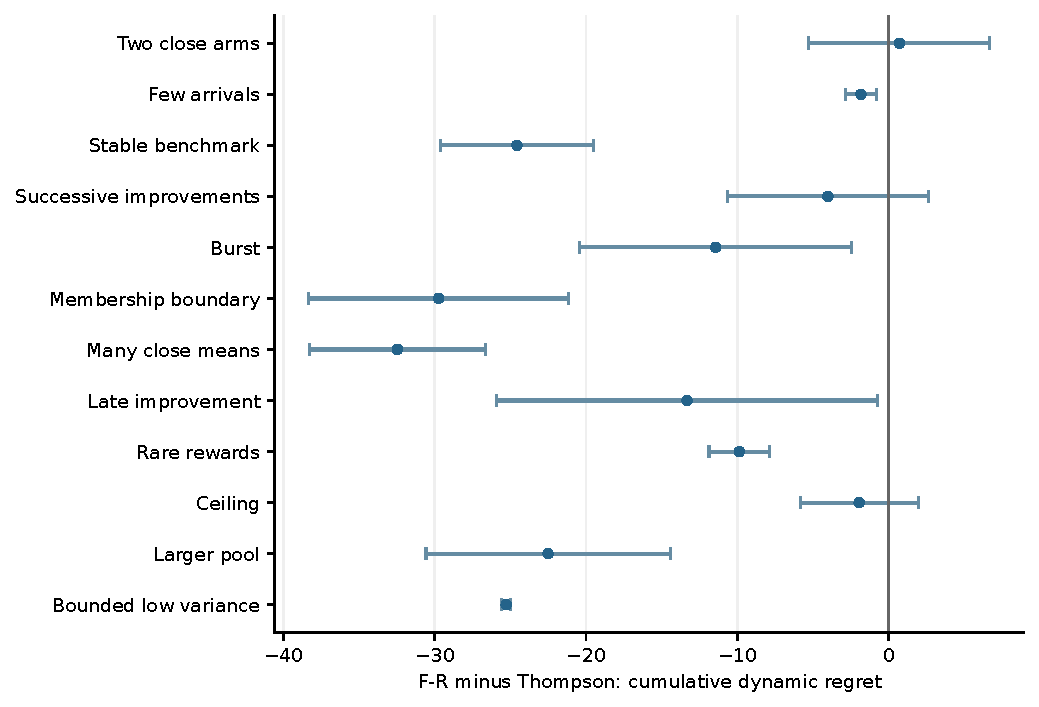
\includegraphics[width=.94\linewidth]{revision2/generated/reward-paired.pdf}
\caption{F-R minus Thompson cumulative dynamic regret in each frozen scenario. Points are means of 96 within-replication differences; error bars are individual two-sided 95\% approximate $t$ intervals. Negative differences favor F-R. These 12 intervals do not by themselves control the 60-comparison family; the adjusted counts are reported in the text.}
\label{fig:reward-paired}
\end{figure}

\subsection{Preference and certification cost}
\begin{table}[t]
\centering
\caption{Descriptive equal-weight averages of the 12 scenario means. The first six rows keep $\beta_C=1$ wherever certification is active; F-area uses no certification cap. Area is in $10^3$ arm-time units. These operating points are not an optimal frontier.}
\label{tab:preference-costs}
\small
\begin{tabular}{llrr}
\toprule
Method / preference & $\beta_C$ & Regret & Area / $10^3$ \\
\midrule
F-R & inactive & 60.73 & 62.22 \\
F, $\lambda=0.1$ & $1$ & 114.68 & 48.29 \\
F, $\lambda=0.3$ & $1$ & 213.55 & 38.46 \\
F, $\lambda=0.6$ & $1$ & 392.99 & 31.70 \\
F, $\lambda=0.9$ & $1$ & 425.03 & 30.84 \\
F, $\lambda=1$ & $1$ & 421.52 & 31.00 \\
F-area & $\infty$ & 1210.02 & 27.12 \\
CCP-original & 1 & 440.32 & 30.07 \\
ALL-auto-costmatched & 1 & 435.68 & 36.72 \\
ALL-area & $\infty$ & 1581.72 & 36.81 \\
\bottomrule
\end{tabular}
\end{table}

Increasing service preference reduces unresolved arm-time over much of the tested range, at a substantial reward cost. The points at $\lambda=.9$ and $1$ under the fixed certification budget are not monotone: the latter has slightly lower regret and slightly larger area. We retain that reversal. F-area removes the certification cap; it is a different budget configuration and is not a continuation of the same-budget curve.

Relative to ALL-auto-costmatched, F-auto-0.6 has lower equal-weight mean regret (392.99 versus 435.68) and area (31.70 versus 36.72 thousand arm-time units). The comparison with CCP-original is a trade-off: F-auto-0.6 has lower mean regret but higher mean area. F-area has lower suite mean regret and area than ALL-area. These are finite-suite averages, rather than per-scenario or pathwise Pareto guarantees. Supplementary Tables~\ref{tab:all-methods} and~\ref{tab:joint-paired} give the scenario decomposition and paired uncertainty.

\begin{figure}[t]
\centering
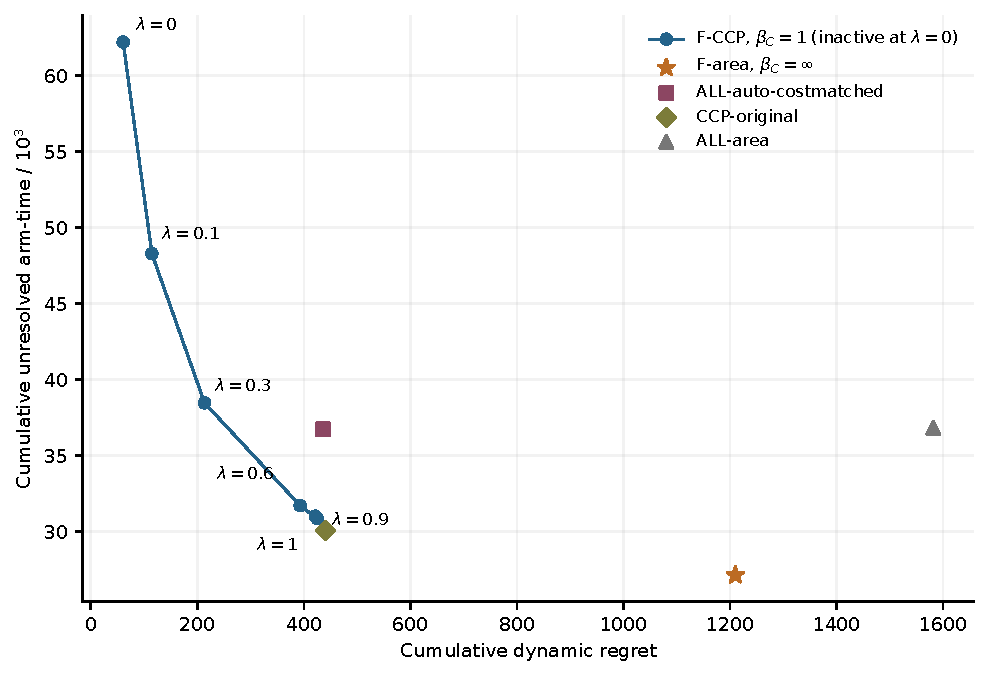
\includegraphics[width=.94\linewidth]{revision2/generated/preference-tradeoff.pdf}
\caption{Descriptive averages of terminal costs over the 12 frozen scenarios. Connected circles follow the prespecified order $\lambda=0,.1,.3,.6,.9,1$, with $\beta_R=16$, temperature $.5$, and $\beta_C=1$ whenever service is active. The star is F-area with $\beta_C=\infty$; the other markers are named comparators. The connecting segments identify configurations and do not estimate a continuous or optimal frontier. Area is divided by $10^3$.}
\label{fig:preference-tradeoff}
\end{figure}

The controller's proposed rate differs from the realized service fraction because the phase must accumulate and the certification guard can reject a proposal. Supplementary Table~\ref{tab:service-diagnostics} reports proposed busy-round rates, successful pulls, denials and the final unresolved count. Fixed-rate, uncapped-service, temperature-one and unprotected-reward variants are retained as prespecified ablations. We use those comparisons only for the mechanisms they actually change.

\subsection{Tail behavior and report failures}
\begin{table}[t]
\centering
\caption{Empirical 95th percentiles of cumulative dynamic regret from 96 replications per method and scenario. These are finite-sample tail summaries, not high-probability regret bounds.}
\label{tab:tail-and-failure}
\small
\begin{tabular}{lrr}
\toprule
Scenario & F-R & Thompson \\
\midrule
Burst & 208.887 & 123.069 \\
Ceiling & 90.940 & 48.971 \\
Larger pool & 237.301 & 184.175 \\
\bottomrule
\end{tabular}
\end{table}

The lower mean regret of F-R does not extend to all tail summaries. Its empirical 95th percentile exceeds Thompson's in the burst, ceiling and larger-pool scenarios in Table~\ref{tab:tail-and-failure}. Each percentile uses only 96 replications; it should not be read as a precise population tail estimate.

F-auto-0.6 produces an incorrect determined label on one of its 1,152 runs; F-R and F-area produce none. Coverage failures and empty intersections also occur: the respective counts are $(6,1)$ for F-R, $(7,1)$ for F-auto-0.6, and $(8,0)$ for F-area. An empty intersection triggers persistent all-unresolved reporting, not successful completion. All these runs enter the cost calculations. Since methods share potential streams, their failures are dependent and cannot be pooled as independent reliability trials. These empirical counts neither replace the reliability theorem nor justify an all-times claim from 96 repetitions. Full failure counts, empirical maxima and implementation qualifications appear in Supplementary Sections~\ref{sec:main-numerical-protocol}--\ref{sec:development-audit}.
\section{Discussion}
\label{sec:discussion}

Reliable maintenance has costs that reward allocation alone does not
measure. An uncertain arrival can obstruct many positive reports, while
a later improvement can end a fine membership task. The general lower
bounds quantify these effects. The worst-area lower bound answers a
different question and is already attained by an initial static batch;
the fixed-schedule and terminal-count growth consequences retain
different quantifiers.

F-CCP adds an implementable choice of emphasis to this task. Its evidence
layer uses every observation, its certificate planner proposes a single
next observation, and separate accounts control reward and certification
costs. Finite guards protect the spectral regret order but can reject
service; the area bound retains that rejection cost. Classification
priority with no certification guard achieves the worst-area order,
without being fastest on every instance. A compatibility endpoint
recovers a specified baseline from the start under identical state and
randomization. The default cold-temperature reward mode has a different
contract.

The frozen experiments support lower mean reward costs for F-R in most
of the specified comparisons and useful finite-budget trade-offs for
the service modes. They also show an exception in the two-arm close-mean
case, heavier empirical regret tails than Thompson sampling in three
environments, and a nonzero label-error record for the balanced mode.
Pure-reward improvements cannot be attributed to certificate scheduling
that was switched off. The corrected matched-cost ALL comparison is
distinct from the retained superseded controller result. These findings
concern the frozen suite, not uniform dominance or a general frontier.

The activation-budgeted witness characterizes an intermediate interval
on a sufficiently separated family, with an additive reward term and
its own information requirements. General causal frontiers under
unknown and overlapping arrivals remain open. The schedule-information
separation does not make every causal comparison impossible. Likewise,
the one-step zero-remainder counterexample leaves room for comparisons
with an explicit adaptation cost or a restricted performance family.

Automatic precision, reward kernels with better tail behavior, a faithful
adaptation of the original ALL-$\varepsilon$ algorithms, and large-pool
planning costs need further study. The supplement's eventual exact-set
consistency theorem belongs to a separate revisable multiresolution
procedure under finite final arrivals and strict boundary separation.
F-CCP's coverage-event completion outside a boundary band is a different
statement.

\section*{Data and code availability}
\enlargethispage{\baselineskip}
The accompanying materials contain simulated data, frozen configurations,
code, and the scripts used to generate the article's tables and figures.
The principal test has 27,648 recorded runs; a subsequent 1,152-run
matched-cost ALL correction is retained separately, together with the
superseded comparator. Replacing that comparator for the principal
analysis leaves 24 configurations and 27,648 records. Earlier checkpoint
comparisons contain 5,760 records and are reported separately in the
supplement; the preceding CCP and frontier research suites retain their
own protocols and archives. All reported failures remain in the analysis.
The available implementation distinguishes the frozen dual-account
production engine from the interactive interface and the development
branches. These materials are provided locally with the project; no
public repository or permanent archive identifier has been verified for
this version.

% ============================================================================
% BEGIN MERGED SUPPLEMENTARY MATERIAL
% ============================================================================
\FloatBarrier
\clearpage
\setcounter{section}{0}
\setcounter{equation}{0}
\setcounter{figure}{0}
\setcounter{table}{0}
\setcounter{algorithm}{0}
\setcounter{page}{1}
\renewcommand{\thesection}{S\arabic{section}}
\renewcommand{\theequation}{S\arabic{equation}}
\renewcommand{\thefigure}{S\arabic{figure}}
\renewcommand{\thetable}{S\arabic{table}}
\renewcommand{\thealgorithm}{S\arabic{algorithm}}
\renewcommand{\thepage}{S-\arabic{page}}
\renewcommand{\theHsection}{supp.\arabic{section}}
\renewcommand{\theHsubsection}{\theHsection.\arabic{subsection}}
\renewcommand{\theHsubsubsection}{\theHsubsection.\arabic{subsubsection}}
\renewcommand{\theHequation}{supp.\arabic{equation}}
\renewcommand{\theHfigure}{supp.\arabic{figure}}
\renewcommand{\theHtable}{supp.\arabic{table}}
\providecommand{\theHalgorithm}{}
\renewcommand{\theHalgorithm}{supp.\arabic{algorithm}}
\renewcommand{\theHtheorem}{\theHsection.\arabic{theorem}}
\phantomsection
\pdfbookmark[0]{Supplementary material}{supplementary-material}
\begin{center}
{\Large\bfseries Supplementary material\par}
\medskip
{\large The Cost of Reliable Near-Optimal Set Maintenance\\with Arriving Arms\par}
\end{center}
\medskip

\section*{Notation and scope}
The observation model has independent arm streams, each consisting of
independent, identically distributed rewards in $[0,1]$, deterministic
permanent arrivals $\mathcal A_t$, and one observation per physical time step.
Each finite $\mathcal A_t$ is nonempty, and arbitrarily large finite batches
are allowed. Arrivals occur before the action, and reports follow its
observation. Let $r^*(t)=\max_{i\in\mathcal A_t}r_i$,
$\Delta_i(t)=r^*(t)-r_i$, and
$\mathcal G_t^\varepsilon=\{i\in\mathcal A_t:\Delta_i(t)\le\varepsilon\}$.
Reports partition $\mathcal A_t$ as
$(\mathcal P_t,\mathcal N_t,\mathcal V_t)$. Write
\[
 E_{\rm lab}=\{\forall t:\mathcal P_t\subseteq\mathcal G_t^\varepsilon
                      \subseteq\mathcal A_t\setminus\mathcal N_t\},\qquad
 \mathcal U_T(\eta)=\sum_{t\le T}\sum_{i\in\mathcal A_t}
 \ind\{i\in\mathcal V_t,|\Delta_i(t)-\varepsilon|>\eta\},
\]
and $R_T=\sum_{t\le T}\Delta_{I_t}(t)$. Reliability means
$P(E_{\rm lab})\ge1-\delta$ for every allowed environment.
$\mathfrak R_\Theta(a)$ minimizes worst-case $ER_T$ over full-model reliable
policies with $P_\vartheta(E_{\rm lab},\mathcal U_T\le a)\ge1-\delta$ for all
$\vartheta\in\Theta$. A bar denotes averaging under the independent uniform
prior on all candidate signs. These priors are proof devices and impose no
Bayesian requirement on the policy.

The probability and sample-budget arguments are given below. Classical
change of measure and multiple-recovery scales are credited to the existing
literature \citep{kaufmann2016,malloy2014,jamieson2018,mason2020}.

% Reorganized from the frozen October 15, 2026 supplement.

\makeatletter
\renewcommand{\@pnumwidth}{2.8em}
\renewcommand{\@tocrmarg}{3.8em}
\renewcommand{\l@section}{\@dottedtocline{1}{0em}{3em}}
\renewcommand{\l@subsection}{\@dottedtocline{2}{1.5em}{4em}}
\renewcommand{\l@subsubsection}{\@dottedtocline{3}{3.8em}{5em}}
\makeatother
\renewcommand{\contentsname}{Supplementary contents}
\addtocontents{toc}{\protect\setcounter{tocdepth}{2}}
\tableofcontents
\medskip
\section{Probability tools and risk conventions}
\label{app:tools}

For the reporting constructions, index arms in arrival order
$i=1,2,\ldots$, with a fixed order within each batch.
Every arm has an independent potential reward stream $(Y_{i,n})_{n\ge1}$
in $[0,1]$. The policy observes its $n$th entry on its $n$th pull. Arrival
times are deterministic, and reports are issued after the current observation.
Write $N_i(t)$ for lifetime observations through round $t$ and
$\hat r_i(n)=n^{-1}\sum_{s\le n}Y_{i,s}$. The observed reward in physical-time notation is
$X_{t,I_t}=Y_{I_t,N_{I_t}(t-1)+1}$. The conclusions below also
hold conditionally on an independent exogenous arrival schedule.

For independent $[0,1]$ observations, Hoeffding's inequality gives
\[
 P\{|\hat r_i(n)-r_i|>x\}\le2e^{-2nx^2}.
\]
For completeness, the centered log moment generating function has value and
derivative zero at the origin; its second derivative is a variance under an
exponentially tilted distribution and is at most $1/4$. Integrating twice
gives $Ee^{\lambda(X-EX)}\le e^{\lambda^2/8}$. Multiplication over independent
observations and exponential Markov inequality prove the display.

For two Bernoulli mean vectors $\boldsymbol r=(r_i)_i$ and
$\boldsymbol r'=(r_i')_i$ and a bounded stopping time $\tau$, action
kernels, policy randomization, and stopping kernels cancel in the history
likelihood ratio. Padding after stopping by null symbols and taking iterated
expectations yields
\begin{equation}
 D(P_{\boldsymbol r}^{H_\tau}\Vert P_{\boldsymbol r'}^{H_\tau})
 =\sum_iE_{\boldsymbol r} N_i(\tau)\operatorname{kl}(r_i,r_i').
 \label{eq:app_kl_identity}
\end{equation}
The same proof applies to arbitrary observation laws with finite two-way KL.
For an event $F$ measurable at stopping, splitting the likelihood integral
over $F,F^c$ and applying Jensen gives
\[
 D(P\Vert Q)\ge\operatorname{kl}(P(F),Q(F))
 \ge P(F)\log\frac1{Q(F)}-\log2.
\]
The second inequality uses the binary entropy bound $h(p)\le\log2$. We repeatedly use
\[
 2(p-q)^2\le\operatorname{kl}(p,q)
 \le\frac{(p-q)^2}{q(1-q)}.
\]
The upper bound follows from $\log x\le x-1$; for the lower bound the second
derivative in $p$ is $1/\{p(1-p)\}\ge4$ and both value and derivative vanish
at $p=q$.

% Reorganized from the frozen October 15, 2026 supplement.

The primary risk combines an unconditional expectation for $R_T$ with a
joint high-probability requirement for labels and unresolved area at each
fixed deterministic endpoint. A common coverage event can yield upper
bounds simultaneously in all endpoints; it does not change the quantifiers
in the lower-bound risk. The fixed-checkpoint, all-prefix, and mixed-evidence
reporters below have separate failure conventions. In particular, the
historical all-prefix convention in Section~\ref{app:legacy-prefix} is not
the persistent-failure convention of F-CCP.
\section{Sequential evidence and certificate planning}\label{app:fccp-evidence}
This section establishes the evidence statements used by F-CCP. The
bounds hold under the bounded iid model and do not require Bernoulli
rewards. All random counts refer to the original potential streams;
no distributional assertion is made conditional on a selected count.

\subsection{The bounded-reward mixture}
Fix a stream of mean $m\in(0,1)$ and let its first $n$ rewards be
$Y_1,\ldots,Y_n\in[0,1]$. For $\vartheta\in(0,1)$ put
\[
 f_{m,\vartheta}(x)=
 (\vartheta/m)^x\{(1-\vartheta)/(1-m)\}^{1-x}.
\]
This is the exponential of an affine function of $x$, hence convex.
The chord inequality on $[0,1]$, followed by conditional expectation,
gives
\[
 \E\{f_{m,\vartheta}(Y_n)\mid Y_1,\ldots,Y_{n-1}\}
 \le(1-m)\frac{1-\vartheta}{1-m}
       +m\frac{\vartheta}{m}=1.
\]
Consequently $\prod_{r\le n}f_{m,\vartheta}(Y_r)$ is a nonnegative
supermartingale. Integrating against the Beta$(1/2,1/2)$ density and
using conditional Tonelli gives another nonnegative supermartingale,
initially one, whose value is
\[
 \mathsf M_n(m)=
 \frac{\operatorname B(\Sigma_n+1/2,n-\Sigma_n+1/2)}
 {\operatorname B(1/2,1/2)m^{\Sigma_n}(1-m)^{n-\Sigma_n}}.
\]
For a nonnegative supermartingale initially one, stop at the first
crossing of $1/\alpha$ before a deterministic integer $L$. The stopped
expectation is at most one, so the crossing probability is at most
$\alpha$. Letting $L$ increase proves Ville's inequality
\[
 \Prob\{\exists n\ge1:\mathsf M_n(m)>1/\alpha\}\le\alpha.
\]
The possible distinction between strict and non-strict crossings is
resolved by taking limits. At $m=0$ or $1$, boundedness forces the stream
to be identically that endpoint almost surely; the formula and inversion
use their limits. In particular, the true endpoint cannot be lost.

For a fixed positive count, the log of $\mathsf M_n(m)$ is a constant
minus $\Sigma_n\log m+(n-\Sigma_n)\log(1-m)$. It is convex in $m$,
so its sublevel set is an interval, possibly empty. Intersecting these
sets over observed prefixes retains simultaneous coverage. The union
bound over arrival ranks gives total mixture failure probability at
most $\sum_i\alpha_i=\delta/2$. Adaptive actions reveal prefixes of
these streams; they cannot invalidate an event defined simultaneously
for every potential prefix. Independent policy randomization can be
included in the physical filtration without altering this argument.

At the deterministic per-arm prefix $q_i$, Hoeffding's inequality gives
\[
 \Prob\{|\hat r_i(q_i)-r_i|>\rho/2\}
 \le2e^{-q_i\rho^2/2}\le\frac{\delta}{2i(i+1)}.
\]
This prefix is defined even when the actual experiment never reaches it.
A second union bound costs at most $\delta/2$. The two types of evidence
need not be independent. On their common event $\mathcal E$, of
probability at least $1-\delta$, every intersection contains its true
mean at every physical time, and any arm that has reached $q_i$ has
interval width at most $\rho$ forever afterward. The failure flag is
never set on $\mathcal E$.

\subsection{Exact rectangular gap bounds and paused work}
Fix a nonempty rectangle
$\mathcal R=\prod_{i\in\mathcal A}[\ell_i,u_i]$.
For $K>1$, minimizing $\max_jr_j-r_i$ over $\mathcal R$ sets
$r_i=u_i$ and every other coordinate to its lower endpoint. Maximizing
it sets $r_i=\ell_i$ and every other coordinate to its upper endpoint.
The resulting extrema are exactly
\[
 g_i^-=\max\{0,\max_{j\ne i}\ell_j-u_i\},\qquad
 g_i^+=\max\{0,\max_{j\ne i}u_j-\ell_i\}.
\]
For $K=1$ the gap is identically zero, regardless of interval width.
This explains why using the same arm's upper and lower endpoints as
independent competitors would be unnecessarily conservative.
The extrema are attained. If
$g_i^-\le\varepsilon<g_i^+$, the rectangle contains both membership
possibilities, so no definite label follows from this rectangle alone.
This is a logical property of rectangular information, not optimality
among all sequential tests or all joint confidence regions.

On $\mathcal E$ the true mean vector lies in $\mathcal R$, which proves
Proposition~\ref{prop:fccp-report}. If
$[g_i^-,g_i^+]\subseteq[\varepsilon-\eta,\varepsilon+\eta]$, the true
gap satisfies $|\Delta_i-\varepsilon|\le\eta$. Such an arm remains in
$\mathcal V$ but contributes no charged area. At a fixed physical time
after arrivals, the subsequent observation only shrinks the rectangle.
Thus its attainable gap intervals only shrink. An arm already given a
definite label cannot become unresolved during this update, and an arm
in the paused set $Z$ cannot return to $W$ during it. Every post-action
arm contributing area therefore belonged to the pre-action $W$.
New arrivals can change this conclusion across rounds, which is why
reports and paused work are always recomputed.

If every available interval has width at most $\rho$, then
\[
 g_i^+-g_i^-\le(u_i-\ell_i)+
                  \max_{j\ne i}(u_j-\ell_j)\le2\rho=\eta/2.
\]
For a still-unresolved arm the gap interval crosses $\varepsilon$.
It is consequently contained in the boundary band, and the arm belongs
to $Z$. Hence $W=\varnothing$ when all current checkpoints are complete.
Equivalently, on $\mathcal E$, nonempty $W$ implies that an incomplete
checkpoint exists and the service fallback can find one.

\subsection{Solution of the two-endpoint planning problem}
Let $n_k^0=\max(1,n_k)$ for $k=i,j$, let
$a_k=v_k^{\mathrm{plan}}\sqrt{n_k^0}$, and fix positive prices $c_k$
and $h>0$. If
$a_i/\sqrt{n_i^0}+a_j/\sqrt{n_j^0}\le h$, the unique minimum of
\eqref{eq:fccp-pair} has $x_k=n_k^0$ and zero proxy cost. Otherwise,
with both $a_k>0$, the active constraint has Lagrange conditions
\[
 c_k=\frac{\omega a_k}{2x_k^{3/2}},\qquad k=i,j,
\]
for every coordinate above its lower bound. If both coordinates are
interior, substitution gives
\begin{equation}\label{eq:fccp-pair-solution}
 D=\frac{a_i^{2/3}c_i^{1/3}+a_j^{2/3}c_j^{1/3}}h,\qquad
 x_k=D^2(a_k/c_k)^{2/3},\quad k=i,j.
\end{equation}
The feasible set is closed, convex, and nonempty; positive prices make
its objective sublevel sets compact. If the interior candidate is below
$n_i^0$, fix $x_i=n_i^0$ and take
\[
 x_j=\max\{n_j^0,(a_j/(h-v_i^{\mathrm{plan}}))^2\}.
\]
The denominator is positive in this boundary case. Exchange $i,j$ for
the other boundary case. When work is needed, both unconstrained
coordinates cannot lie below their lower bounds. Equivalently, the
solution is characterized by
\[
 x_k(\omega)=\max\{n_k^0,(\omega a_k/(2c_k))^{2/3}\},
 \qquad \sum_k a_k/\sqrt{x_k(\omega)}=h.
\]
The radius sum decreases strictly after leaving its initial plateau,
which proves uniqueness. A zero $a_k$ leaves that coordinate at its
lower bound and reduces the problem to the other coordinate. With two
zero radii no work is needed.

In the service routine, a legal endpoint additionally requires
$n_k<q_k$ and $x_k>n_k$, using the actual count in this comparison.
Among its two legal endpoints, choose the larger
$v_k^{\mathrm{plan}}/(\max(1,n_k)c_k)$; a tie favors the current
candidate $i$. Scan candidates in arrival order and retain the first
pair of minimum cost. Empirical-best and largest-upper reference ties
also use first arrival. If no legal pair is found, scan incomplete
checkpoints for the first interval of largest width. These conventions
specify the deterministic pair-plan routine used by the main algorithm.
The convention $\max(1,n_k)$ neither increments $n_k$ nor shrinks the
report interval. The proxy's frozen centers and assumed radius decay
are not assertions about future random observations.

The numerical implementation replaces zero planning radii by
$10^{-12}$, uses a $10^{-8}$ tolerance for positive planned increments,
and retains the original actual counts for all statistical updates.
Its fixed-prefix evidence is not altered by these numerical conventions.
\section{Virtual indices and the optimism-gap bound}\label{app:optimism-gap}
We give the arbitrary-action bridge used in
Theorem~\ref{thm:fccp-budget}. The potential-prefix and arrival-clock
arguments originate in the companion manuscript
\citet{temporalgeometry2026}. Their use here must allow actions that do
not maximize the virtual index. No confidence-success conditioning is
used anywhere in this section.

\subsection{Potential-prefix bounds}
For one original potential stream of mean $r$, write
$S_n=\sum_{v=1}^n(r-Y_v)$ in this subsection only, and define
\[
 Z(v)=\sup_{n\ge1}\left[r-\hat r(n)-
                \sqrt{[\log(v/n)]_+/n}\right]_+,
 \qquad v>0.
\]
The symbol $S_n$ here is a centered partial sum, not the reward sum
$\Sigma_i$ or the arrival spectrum $\mathcal S_t$.
For bounded rewards Hoeffding's moment bound gives
$\E e^{\gamma(r-Y_v)}\le e^{\gamma^2/8}$.
Applying the nonnegative-supermartingale crossing inequality to
$e^{\gamma S_n-n\gamma^2/8}$ yields
\begin{align}
 \Prob\{\exists n>v:S_n/n\ge x\}&\le e^{-2vx^2},
       &&v,x>0,\label{eq:fccp-large-prefix}\\
 \Prob\{\max_{n\le L}S_n\ge y\}&\le e^{-2y^2/L},
       &&L\in\mathbb N,\ y>0.\label{eq:fccp-prefix-max}
\end{align}
For the first inequality use $\gamma=4x$; for the second use
$\gamma=4y/L$. The first event is an infinite union of countable
prefixes, obtained by increasing finite stopping horizons.

\begin{lemma}[Potential underestimation]\label{lem:fccp-Z}
For every $v>0$, $\E Z(v)\le5/\sqrt v$.
\end{lemma}
\begin{proof}
Use \eqref{eq:fccp-large-prefix} for $n>v$. For $n\le v$, let
$m_k=v2^{-(k+1)}$ and partition the positive integer counts into
$m_k<n\le2m_k$, $k\ge0$. If a prefix in this interval makes
$Z(v)>x$, then
\[
 S_n>m_kx+\sqrt{m_kk\log2}.
\]
For a nonempty integer interval,
\eqref{eq:fccp-prefix-max} with $L=\lfloor2m_k\rfloor$ bounds its
probability by $2^{-k}e^{-vx^2/2^{k+1}}$. Therefore
\[
 \Prob\{Z(v)>x\}\le e^{-2vx^2}
             +\sum_{k\ge0}2^{-k}e^{-vx^2/2^{k+1}}.
\]
Integrating the nonnegative terms gives
\[
 \E Z(v)\le\frac{\sqrt\pi}{2\sqrt{2v}}+
     \frac{\sqrt\pi}{\sqrt{2v}}\sum_{k\ge0}2^{-k/2}
       <\frac5{\sqrt v}.
\]
This statement is about the original stream simultaneously over its
counts, so it also bounds a count selected using its observed past.
\end{proof}

\Needspace{11\baselineskip}
\begin{lemma}[Distinct arm--count pairs]\label{lem:fccp-distinct}
Select at most $h$ pairs $(i,n)$ from $k$ fixed potential streams,
where $n\ge1$ and no pair is used more than once. The selection may
depend on the entire adaptive experiment. Then
\[
 \E\sum_{\mathrm{selected}\ (i,n)}
              (\hat r_i(n)-r_i)_+\le\sqrt{2kh}.
\]
For every $v>0$,
\[
 \sum_{n\ge1}\sqrt{[\log(v/n)]_+/n}\le\sqrt{2\pi v}.
\]
\end{lemma}
\begin{proof}
For every $x>0$ the first sum is bounded pathwise by
\[
 xh+\sum_{i=1}^k\sum_{n\ge1}(\hat r_i(n)-r_i-x)_+.
\]
The expectation of the double sum for one arm is at most
\[
 \int_x^\infty\sum_{n\ge1}e^{-2ny^2}\,dy
 =\int_x^\infty\frac{dy}{e^{2y^2}-1}\le\frac1{2x}.
\]
Minimize $xh+k/(2x)$ at $x=\sqrt{k/(2h)}$; the empty-selection case
is immediate. This proof does not condition on any chosen empirical
mean. For the second statement the summand decreases on $(0,v)$, so
its sum is at most
\[
 \int_0^v\sqrt{\log(v/x)/x}\,dx
 =\sqrt v\int_0^\infty y^{1/2}e^{-y/2}\,dy
 =\sqrt{2\pi v}.
\]
If $v<1$ the sum is zero, which also satisfies the bound.
\end{proof}

\subsection{A segment with arbitrary actions}
Fix the deterministic arrival schedule, reward laws, and a virtual
clock segment of capacity $d=d_{\mathrm{clock}}$ and prefix length
$h$. The start and end of this segment depend only on arrivals.
At most $k\le d$ arms are available during the segment: its starting
competitor count is $c$, $d=2c$, and any later count $K_t-1\ge2c$
would start a new segment before the action. Retain all samples from
before the segment.

At every time choose a true optimal label $i_t^*$ by a fixed rule using
only the fixed means and schedule. For $n_{i_t^*}>0$, clipping at one
cannot move its index below
$r^*(t)-Z_{i_t^*}(s/d)$, since $r^*(t)\le1$.
For $n_{i_t^*}=0$, its index is one and the same lower bound holds.
For an observed selected arm, the identity
$J_{I_t}=\max_jJ_j-\zeta_t(I_t)$ and the upper bound
$J_{I_t}\le\hat r_{I_t}(n)+\sqrt{[\log\{s/(dn)\}]_+/n}$ give
\begin{equation}\label{eq:fccp-arbitrary-decomposition}
 \Delta_{I_t}(t)\le\zeta_t(I_t)+Z_{i_t^*}(s/d)
       +(\hat r_{I_t}(n)-r_{I_t})_+
       +\sqrt{[\log\{s/(dn)\}]_+/n},\quad n=N_{I_t}(t-1)>0.
\end{equation}
This comparison does not assume that the chosen arm maximizes $J$.
In particular, an unobserved optimal arm creates no exceptional
conditioning issue. The genuinely first pulls of selected arms are
charged separately at cost at most one each.

If $h\ge d$, first pulls cost at most $d\le\sqrt{dh}$.
Lemma~\ref{lem:fccp-Z}, applied to the deterministic label at each
local time, gives
\[
 \sum_{s=1}^h\E Z_{i_t^*}(s/d)
        \le5\sum_{s=1}^h\sqrt{d/s}\le10\sqrt{dh}.
\]
An arm's lifetime count increases at every actual pull, whether it is
called a reward pull or a service pull. Hence its selected pre-pull
count never repeats. Lemma~\ref{lem:fccp-distinct} bounds the empirical
excess by $\sqrt{2dh}$. For bonuses replace $s$ by $h$, extend each
arm's counts to all positive integers, and obtain
$k\sqrt{2\pi h/d}\le\sqrt{2\pi dh}$. Summing proves
\begin{equation}\label{eq:fccp-segment}
 \E R_{\mathrm{segment}}\le
  15\sqrt{dh}+\E\sum_{t\in\mathrm{segment}}\zeta_t(I_t).
\end{equation}
The coefficients sum to
$1+10+\sqrt2+\sqrt{2\pi}<15$. If $h<d$, the trivial regret bound
$h\le\sqrt{dh}$ gives \eqref{eq:fccp-segment} as well. These are
unconditional expectations under the original experiment, so old
observations and arbitrary predictable score kernels are allowed.

\subsection{Deterministic charging of arrival clocks}
For $b>0$ put $f_b(k)=\min\{b,\sqrt{kb}\}$. It is subadditive:
$f_b(\sum_rk_r)\le\sum_rf_b(k_r)$, since a saturated term settles
the assertion and otherwise the square root is subadditive.
We use two deterministic spectral facts from
\citet{temporalgeometry2026}, recording their proofs to fix the interface.

Deleting competitors and delaying the remaining competitors, without
changing the endpoint, produces a spectrum at most twice the original
one. Indeed, arms originally in dyadic group $m$ can only move to
groups $\ell\le m$. If $k_{m,\ell}$ counts these arms, their new total
cost is bounded both by
\[
 \sum_{\ell\le m}2^\ell<2\cdot2^m,\qquad
 \sum_{\ell\le m}\sqrt{k_{m,\ell}2^\ell}
       \le\sqrt{2k_m2^m}.
\]
It is therefore at most $2f_{2^m}(k_m)$. Subadditivity separates the
original groups; summing proves the comparison. Also, if $m$
competitors have lifetime at least $H$, their spectral contribution is
at least $f_H(m)$: each containing group has upper endpoint at least
$H$, and subadditivity combines the groups.

Before the first competitor arrives, regret is zero. Index later
segments by $j=0,\ldots,J$, with starts $\sigma_j$, lengths $h_j$,
starting competitor counts $c_j=K_{\sigma_j}-1$, capacities
$d_j=2c_j$, and remaining lifetimes $H_j=T-\sigma_j+1$.
The counts satisfy $c_{j+1}\ge2c_j$.
If $j_*$ is the first index for which $c_j\ge H_j$, charge that
segment and the entire later tail by $H_{j_*}\le\mathcal S_T$,
using the preceding lifetime fact. If no such index exists, all
segments belong to the following sum.

For $j<j_*$ put $c_{-1}=0$ and retain the competitors arriving between
consecutive segment starts, including initial competitors for $j=0$.
There are $m_j=c_j-c_{j-1}\ge c_j/2$ such arms. Delete all other
competitors and delay these $m_j$ arms to $\sigma_j$; this produces
$\mathcal S_T'\le2\mathcal S_T$. Group the retained starts by the
dyadic scale of $H_j$. For a nonempty group of upper endpoint
$b_\ell=2^\ell$, with last segment $j_{\mathrm{last}}$, geometric
growth gives
\[
 \sum_{j:H_j\in(b_\ell/2,b_\ell]}\sqrt{c_jH_j}
 \le\frac{\sqrt{c_{j_{\mathrm{last}}}b_\ell}}
                  {1-2^{-1/2}}.
\]
The number $k_\ell'$ of delayed competitors in this group satisfies
\[
 c_{j_{\mathrm{last}}}/2\le k_\ell'\le c_{j_{\mathrm{last}}}
           <H_{j_{\mathrm{last}}}\le b_\ell.
\]
Its spectral cost is unsaturated. Therefore, using $h_j\le H_j$,
\[
 \sum_{j<j_*}\sqrt{c_jh_j}
 \le\frac{2\sqrt2}{1-2^{-1/2}}\mathcal S_T.
\]
Together with \eqref{eq:fccp-segment}, the capacities $d_j=2c_j$,
and the tail bound, this yields
\begin{equation}\label{eq:fccp-optimism-proof}
 \E R_T\le
 \left(1+\frac{60}{1-2^{-1/2}}\right)\mathcal S_T
       +\E\sum_{t\le T}\zeta_t(I_t)
 \le300\mathcal S_T+\E\sum_{t\le T}\zeta_t(I_t).
\end{equation}
The nonnegative index-gap terms may be extended from the retained
segments to the whole horizon. Since $R_T\le T$, this proves
\eqref{eq:fccp-optimism}. The endpoint-dependent grouping is used
only in the proof; none of it is an algorithm input.

Finally, for any $u\le T$, remove competitors arriving after $u$ and
delay every remaining competitor by $T-u$. Their ages at $T$ are
exactly their ages at $u$, so the same deletion--delay comparison gives
$\mathcal S_u\le2\mathcal S_T$ and thus
\begin{equation}\label{eq:fccp-running-spectrum}
 \overline{\mathcal S}_T\le2\mathcal S_T.
\end{equation}
The counting anchor is never removed or delayed. Neither this bound
nor the arbitrary-action inequality reestablishes the companion
minimax lower theorem; that theorem is a separately attributed input
when interpreting the regret order.
\section{Guarantees for Flexible CCP}\label{app:fccp-guarantees}
The reward and service results have different hypotheses. Reliability
allows any legal predictable preference, including a preference tending
to zero. The regret bound uses fixed budget coefficients; an area rate
requires a positive lower bound on service while work remains. These
conditions are not supplied by the word ``adaptive.''

\subsection{Compatibility and state preservation}
To prove Proposition~\ref{prop:fccp-compat}, couple the potential reward
streams, arrivals, full initial kernel state, and backend random-number
source. At the first round the service rate is zero, the reward guard
is disabled, and the same kernel receives the same observed state.
Its scores and selected action agree. Both procedures reveal the same
next potential reward from that arm, so the kernel states still agree.
Repeat inductively. The evidence updates do not affect decisions in
this mode and consume no action random numbers. Any auxiliary kernel
state, including its clock and random-number state, must be included
in the coupling. This proves equality of actions, lifetime counts,
and regret simultaneously at every physical round and endpoint.

For standard Beta$(1,1)$ Thompson sampling, this endpoint uses
$\theta=1$, $\lambda=0$, and $\beta_R=\infty$. It does not include
F-R, which has $\theta=.5$ and a finite guard. The batch backend and
interactive backend use different random-number implementations;
matching their numerical seeds is not this coupling. Likewise, a
preference switch after earlier service preserves the actual history,
not the history of a baseline independently run from the beginning.
The interface changes preferences only between a completed observation
and the next action and resets no count, interval, phase, or ledger.

\subsection{The two-ledger regret bound}
For a fixed finite budget coefficient the corresponding budget
$\beta\overline{\mathcal S}_t$ is nondecreasing. Initially each ledger
is zero. On a service round its guard explicitly verifies
$C_C(t-1)+\zeta_t(I_t)\le\beta_C\overline{\mathcal S}_t$;
on other rounds this ledger is unchanged. Induction gives
\[
 C_C(T)\le\beta_C\overline{\mathcal S}_T.
\]
On a reward round the maximization is restricted to
$\mathcal F_R(t)$. This set is nonempty: a largest-index arm has
$\zeta_t=0$, and the previous reward ledger remains within the
nondecreasing budget. Thus
\[
 C_R(T)\le\beta_R\overline{\mathcal S}_T.
\]
This argument also covers $\beta_R=0$ and $\beta_C=0$; only zero-gap
actions can then consume the corresponding type of round. Disabling
a guard means bypassing its comparison, not evaluating
$\infty\cdot0$. All these decisions occur before the sole reward
observation at that physical time.

Every actual round is exactly one of the two types, and therefore
\[
 \sum_{t\le T}\zeta_t(I_t)=C_R(T)+C_C(T)
   \le(\beta_R+\beta_C)\overline{\mathcal S}_T
   \le2(\beta_R+\beta_C)\mathcal S_T.
\]
Apply \eqref{eq:fccp-optimism}. Its expectation includes failed
reporting histories and arbitrary reward scores, so this substitution
does not incur a missing $\delta T$ term. Truncation by $T$ proves
\eqref{eq:fccp-regret-finite}. When service is disabled throughout the run its ledger
is identically zero, which removes $\beta_C$.

Even without the certification guard, every actual service selects
an arm of actual count below $q_i$ and increments that count once.
Lifetime counts are shared with reward allocation and never reset,
so the total number of services through $T$ is at most
$Q_T^{\mathrm{cap}}=\sum_{i\in\mathcal A_T}q_i$ on every path.
The persistent failure rule can only reduce this number. Since
$0\le\zeta_t\le1$, $C_C(T)\le Q_T^{\mathrm{cap}}$.
Combining it with the reward guard and
\eqref{eq:fccp-running-spectrum} proves
\eqref{eq:fccp-regret-unlimited}.

The resulting preset bounds are
\[
 \begin{array}{ll}
 \mathrm{F\!\!\!-R}:&\E R_T\le\min\{T,332\mathcal S_T\},\\
 \mathrm{Balanced}:&\E R_T\le\min\{T,334\mathcal S_T\},\\
 \mathrm{Classification}:&\E R_T\le
                       \min\{T,332\mathcal S_T+Q_T^{\mathrm{cap}}\}.
 \end{array}
\]
The compatibility endpoint has no finite reward-guard coefficient, so
these bounds are not inherited automatically for an arbitrary kernel.
The two ledgers bound observable optimism gaps, not the realized regret
difference from an independently run kernel. The established companion
minimax lower bound supplies the matching spectral order for finite
fixed coefficients, with no assertion of sharp constants or optimality
under a prescribed area constraint.

\subsection{Phase accounting and the area guarantee}
Let $A_T^{\mathrm{att}}$ be the number of designated service attempts
and $B_T^{\mathrm{busy}}$ the number of pre-action rounds with nonempty
$W_t$. In exact arithmetic $0\le\phi_t<1$, because $0\le p_t\le1$
and each crossing causes exactly one subtraction. The telescoping
identity is
\begin{equation}\label{eq:fccp-phase}
 \phi_T=\sum_{t\le T}p_t-A_T^{\mathrm{att}},\qquad
 A_T^{\mathrm{att}}=\left\lfloor\sum_{t\le T}p_t\right\rfloor.
\end{equation}
A service denial does not undo this subtraction and is not retried
within the same physical round.

On $\mathcal E$, Supplement~\ref{app:fccp-evidence} shows that busy
work implies an incomplete checkpoint and hence a legal proposal.
Every attempt is then either an executed service or a certification
budget denial. If $D_T^{\mathrm{srv}}$ counts these denials and
$S_T^{\mathrm{srv}}$ executed services, then
\[
 A_T^{\mathrm{att}}=S_T^{\mathrm{srv}}+D_T^{\mathrm{srv}},\qquad
 S_T^{\mathrm{srv}}\le Q_T^{\mathrm{cap}}.
\]
When $p_t\ge p_{\min}>0$ on busy rounds, the rate is zero on all
other rounds and \eqref{eq:fccp-phase} gives
\[
 p_{\min}B_T^{\mathrm{busy}}\le\sum_{t\le T}p_t
           <Q_T^{\mathrm{cap}}+D_T^{\mathrm{srv}}+1.
\]
Every post-action arm that contributes area was in the pre-action
$W_t$, so $\mathcal U_T(\eta)\le K_TB_T^{\mathrm{busy}}$.
Together with the deterministic $K_TT$ bound, this proves
Theorem~\ref{thm:fccp-area} on the single event $\mathcal E$,
simultaneously for all endpoints. It is a high-probability area
statement, not an expected-area replacement for the model's risk.

For adaptive control $p_0\le w_t\le1$. The function
$\lambda w/(1-\lambda+\lambda w)$ increases in $w$, so a fixed
$\lambda>0$ gives \eqref{eq:fccp-pmin}. Fixed-rate control also obeys
this lower bound. At $\lambda=1$ the rate is one on busy rounds.
When the certification guard is disabled,
$D_T^{\mathrm{srv}}=0$, and
\[
 Q_T^{\mathrm{cap}}=O\{K_T\eta^{-2}\log(K_T/\delta)\}.
\]
Consequently Classification has area
$O(\min\{K_TT,K_T^2\eta^{-2}\log(K_T/\delta)\})$.
The comparison with the retained worst-area lower bound uses its
common range $K_T\ge2$, $\varepsilon\le1/8$,
$\eta\le\varepsilon/32$, and $\delta\le1/16$.
This is an order comparison over the worst environments and schedules;
it does not identify the fastest classification rule on each instance.
Finite certification budgets must retain the denial count. If the
preferences can approach zero without a common positive lower bound,
\eqref{eq:fccp-phase} still holds but gives no bound on the number of
unweighted busy rounds by itself.

\subsection{A finite-arm nonstarvation bound}
Fix an endpoint $T$, write $Q=Q_T^{\mathrm{cap}}$, and suppose
$\beta_C>0$ with a positive busy-round lower rate. On $\mathcal E$,
\begin{equation}\label{eq:fccp-nonstarvation}
 \mathcal U_T(\eta)\le K_T\min\left\{T,
       \left\lceil(Q/\beta_C)^2\right\rceil+1+
                         \frac{Q+1}{p_{\min}}\right\}.
\end{equation}
For a disabled certification guard use the no-denial area bound
instead. To prove \eqref{eq:fccp-nonstarvation}, let $\tau_c$ be
the first time a second arm is available. A singleton is certified
positive without observations, so it contributes no unresolved area.
The first competitor remains available forever. Its current age gives
\[
 \mathcal S_t\ge\sqrt{t-\tau_c+1},\qquad t\ge\tau_c.
\]
Thus after at most $\lceil(Q/\beta_C)^2\rceil+1$ rounds from
$\tau_c$, the certification budget is at least $Q$. Before that
point charge all busy rounds by this length.

If a service proposal is still legal, fewer than $Q$ services have
occurred: otherwise all quotas of the prefix would already have been
reached, even without counting reward pulls. The ledger plus the next
service gap is at most the previous service count plus one, and
therefore at most $Q$. Once the budget reaches $Q$, no remaining
service can be rejected. Over any subsequent interval the inherited
phase can only help; phase accounting bounds its remaining busy rounds
by $(Q+1)/p_{\min}$. Combining the two parts proves
\eqref{eq:fccp-nonstarvation}.

If arrivals eventually stop, use the final finite value of $Q$.
The budget eventually exceeds $Q$ and the number of further busy
rounds is finite. After the final arrival the confidence rectangles
only shrink, so a persistently unresolved arm outside the boundary
band would require infinitely many busy rounds, a contradiction.
This proves Corollary~\ref{cor:fccp-finite}. The reward ledger does
not enter the argument; continuing reward exploration cannot consume
the separately reserved certification budget. The bound is
conservative and is not a worst-area matching result for finite
budgets. It applies on $\mathcal E$ and leaves the boundary band
unrestricted, so it is not unconditional almost-sure exact-set
consistency. When $\beta_C=0$ this proof provides no eventual-service
guarantee.

\subsection{Why compatibility does not imply universal dominance}
Consider two initially available arms, one physical round, and two
specified baselines. Baseline A is MC-MOSS with the stated fixed-label
initialization and chooses arm 1 first. Baseline B is symmetric
Beta$(1,1)$ Thompson sampling and chooses either arm with probability
$1/2$. Let an arbitrary unknown-mean policy choose arm 1 with
probability $p$. In the bounded environment $(r_1,r_2)=(3/4,1/4)$,
its expected regret exceeds that of the best specified baseline by
$(1-p)/2$. In environment $(1/4,3/4)$, the excess is $p/2-1/4$.
The first decision has the same information in the two environments,
and
\[
 \min_{p\in[0,1]}\max\{(1-p)/2,\,p/2-1/4\}=1/8,
\]
attained at $p=3/4$. Thus no unknown-mean procedure is exactly no worse
than both baselines in every environment and at every endpoint with
zero remainder. This example concerns these initializations and that
literal requirement. It does not preclude comparisons with an
adaptation cost, asymptotic noninferiority, spectral minimax rates,
or finite-suite numerical improvements.

\subsection{Implementation arithmetic and branch identity}
The mathematical contract uses exact interval inversion, phase
arithmetic, and budget comparisons. The frozen implementation uses
35 bisection steps with outward mixture endpoints and a $10^{-12}$
budget-comparison tolerance. Planning regularization was described in
Supplement~\ref{app:fccp-evidence}. At a cumulative phase close to an
integer, floating addition can delay an attempt by one round. These
choices belong to the numerical implementation; the displayed exact
phase identity is not asserted as a bitwise identity for every floating
trajectory.

The production batch rule has two ledgers. If a proposed service fails
its certification check, it draws the chosen reward kernel's scores
once and maximizes them over the reward-feasible set. It does not
necessarily choose a largest-MC-index arm. No unexecuted proposal
reveals a reward. Each completed choice is followed by exactly one
physical observation and one update to the selected arm's actual
count and sum. The earlier single-ledger development branch is not
this production rule. The interactive interface implements the same
dual-budget decision contract; its corrected ALL-controller wrapper
changes only that comparator's observed proposal-cost input and does
not alter the F-CCP branch.
\section{Checkpoint-UCB as an attainability witness}
\label{app:checkpoint_construction}

The original explicit upper bounds use Checkpoint-UCB as a fixed-precision
attainability witness. It is distinct from F-CCP in its evidence, service
schedule, and reward rule. Its
reporting intervals are formed once, while its reward estimates use every
observation. Index arms by arrival order $i=1,2,\ldots$, with a fixed order
within each batch. Choose $0<\rho<1$ before observing rewards and set
\begin{equation}
 q_i(\rho)=\left\lceil\frac2{\rho^2}
                  \log\frac{4i(i+1)}\delta\right\rceil.
 \label{eq:checkpoint}
\end{equation}
Before this lifetime count is reached, arm $i$ has reporting interval $[0,1]$.
At its $q_i$th observation the interval becomes permanently
\begin{equation}
 [\ell_i,u_i]=[\hat r_i(q_i)-\rho/2,
                 \hat r_i(q_i)+\rho/2]\cap[0,1].
 \label{eq:fixed_interval}
\end{equation}
Although its completion time is adaptive, the
interval uses a predetermined potential prefix. Different precisions
$\rho_i$ may also be prescribed before the corresponding arms are observed;
data-dependent checkpoint selection is not covered.

At even times the policy serves the first incomplete checkpoint in arrival
order, if one remains. At every other time it maximizes, over all
$i\in\mathcal A_t$,
\begin{equation}
 J_i(t)=\hat r_i(N_i(t-1))+
             \sqrt{\frac{3\log(2t)}{N_i(t-1)}}.
 \label{eq:ucb}
\end{equation}
A zero count gives index $+\infty$; ties are broken by the smallest
arrival-order label. Both kinds of pull update the same count and reward
sum. After observing the selected reward, define
$\underline r^*(t)=\max_{i\in\mathcal A_t}\ell_i$ and
$\overline r^*(t)=\max_{i\in\mathcal A_t}u_i$, and report
\begin{equation}
 \mathcal P_t=\{i:\ell_i\ge\overline r^*(t)-\varepsilon\},\qquad
 \mathcal N_t=\{i:u_i<\underline r^*(t)-\varepsilon\},\qquad
 \mathcal V_t=\mathcal A_t\setminus(\mathcal P_t\cup\mathcal N_t).
 \label{eq:reports}
\end{equation}

\begin{algorithm}[p]
\caption{Checkpoint-UCB}
\label{alg:checkpoint-ucb}
\begin{algorithmic}[1]
\Require $\varepsilon\in(0,1)$, $\delta\in(0,1/2)$, predetermined $\rho\in(0,1)$
\State $\mathcal A^{\rm cur}\gets\varnothing$, FIFO queue $\mathcal Q^{\rm srv}\gets\varnothing$, $k\gets0$
\For{physical time $t=1,2,\ldots$}
  \For{each arm arriving at $t$, in a fixed within-batch order}
    \State $k\gets k+1$; assign label $i\gets k$; $\mathcal A^{\rm cur}\gets\mathcal A^{\rm cur}\cup\{i\}$
    \State $n_i\gets0$, $s_i\gets0$, $[\ell_i,u_i]\gets[0,1]$
    \State $q_i\gets\left\lceil(2/\rho^2)\log\{4i(i+1)/\delta\}\right\rceil$; append $i$ to $\mathcal Q^{\rm srv}$
  \EndFor
  \While{$\mathcal Q^{\rm srv}\ne\varnothing$ and $n_{\operatorname{front}(\mathcal Q^{\rm srv})}\ge q_{\operatorname{front}(\mathcal Q^{\rm srv})}$}
    \State Remove the front of $\mathcal Q^{\rm srv}$
  \EndWhile
  \If{$t$ is even and $\mathcal Q^{\rm srv}\ne\varnothing$}
    \State $I\gets\operatorname{front}(\mathcal Q^{\rm srv})$ \Comment{designated service pull}
  \Else
    \State $J_i\gets+\infty$ if $n_i=0$, and $J_i\gets s_i/n_i+\sqrt{3\log(2t)/n_i}$ otherwise, for $i\in\mathcal A^{\rm cur}$
    \State $I\gets\min\operatorname*{arg\,max}_{i\in\mathcal A^{\rm cur}}J_i$
  \EndIf
  \State Pull $I$ once and observe $x$; $n_I\gets n_I+1$, $s_I\gets s_I+x$
  \If{$n_I=q_I$}
    \State $m\gets s_I/q_I$; $\ell_I\gets\max\{0,m-\rho/2\}$, $u_I\gets\min\{1,m+\rho/2\}$
  \EndIf
  \State $L\gets\max_{i\in\mathcal A^{\rm cur}}\ell_i$, $U\gets\max_{i\in\mathcal A^{\rm cur}}u_i$
  \State $\mathcal P_t\gets\{i\in\mathcal A^{\rm cur}:\ell_i\ge U-\varepsilon\}$, $\mathcal N_t\gets\{i\in\mathcal A^{\rm cur}:u_i<L-\varepsilon\}$
  \State $\mathcal V_t\gets\mathcal A^{\rm cur}\setminus(\mathcal P_t\cup\mathcal N_t)$; report $(\mathcal P_t,\mathcal N_t,\mathcal V_t)$
\EndFor
\end{algorithmic}
\end{algorithm}

Algorithm~\ref{alg:checkpoint-ucb} observes exactly one reward per physical
round. Its variables $n_i$ and $s_i$ are the lifetime count and reward sum.
An ordinary UCB pull can complete any checkpoint, including one behind the
queue's front. The queue discards such completed entries when they reach its
front. An interval is computed only when $n_i=q_i$, and is not recomputed
when $n_i>q_i$. Reaching $q_i$ forms fixed-precision evidence; it need not
produce a determinate report if other arms are still uncertain or the arm
lies closer to the boundary than that evidence can resolve.

All arrived arms remain eligible for \eqref{eq:ucb}, including negatively
reported arms. The intervals are nonempty on every path, so
$\mathcal P_t$ and $\mathcal N_t$ are disjoint. A count, sum, and interval
are stored for every arm; a direct index or report update costs $O(K_t)$
operations. The policy uses no terminal horizon, future arrivals, true means,
or reference identities.

\begin{proposition}[Simultaneous reporting and unconditional reward cost]
\label{prop:reporting}
On the full bounded model, Checkpoint-UCB satisfies
$\Prob(E_{\rm lab})\ge1-\delta/2$. If $\mathcal I_T$ is its set of designated
service time steps, then at every deterministic $T$,
\begin{equation}
 \E R_T\le\min\left\{T,K_T+4\sqrt{3K_TT\log(2T)}+1+
                \E\sum_{t\in\mathcal I_T}\Delta_{I_t}(t)\right\}.
 \label{eq:reward_bound}
\end{equation}
Pathwise, $|\mathcal I_T|\le\sum_{i\le K_T}q_i$.
\end{proposition}


\subsection{Reporting proof and fixed-prefix evidence}
The sum of coverage failures is at most
$\sum_i\delta/\{2i(i+1)\}=\delta/2$. On coverage, each endpoint differs from
the true mean by at most $\rho_i$. These intervals are nonempty on every path
and only contract once. If $\underline r^*(t)=\max_i\ell_i(t)$ and
$\overline r^*(t)=\max_i u_i(t)$, use
\[
 \mathcal P_t=\{i:\ell_i(t)\ge\overline r^*(t)-\varepsilon\},\quad
 \mathcal N_t=\{i:u_i(t)<\underline r^*(t)-\varepsilon\},\quad
 \mathcal V_t=\mathcal{A}_t\setminus(\mathcal P_t\cup \mathcal N_t).
\]
The sets $\mathcal P_t,\mathcal N_t$ are disjoint because
$\underline r^*(t)\le\overline r^*(t)$ and $\ell_i\le u_i$.
Coverage implies
$\mathcal P_t\subseteq \mathcal G_t^\varepsilon\subseteq \mathcal{A}_t\setminus \mathcal N_t$.
Moreover, $\mathcal N_t$ is increasing as observations and arrivals accumulate:
$\underline r^*(t)$ cannot decrease and an existing $u_i$ cannot increase.


\subsection{Unconditional reward and completion guarantees}
\label{app:joint}
\paragraph{A reward bound that does not condition on report coverage.}
At physical time $t$, order arms by their first observed rewards. At most
$t$ streams have been exposed, each at at most $t$ potential prefixes. A
previously unobserved stream is independent of the history selecting it.
Applying Hoeffding to each newly exposed stream and union bounding gives
\[
 P\left\{\exists\text{ observed arm and prefix }n\le t:
 |\hat r_i(n)-r_i|>
        \sqrt{3\log(2t)/n}\right\}
 \le2t^2(2t)^{-6}=\frac1{32t^4}.
\]
The exposure order is used only for this union bound, not to assert
independence among observed counts. An ordinary UCB pull with finite index,
on this event's complement, has
$\Delta_{I_t}(t)\le2\sqrt{3\log(2t)/N_{I_t}(t-1)}$.
Each arm--pre-pull-count pair is charged at most once; interleaved service
observations skip counts. Therefore the ordinary, nonfirst-pull regret is
at most
\[
 4\sqrt{3\log(2T)}\sum_i\sqrt{N_i(T)}
 \le4\sqrt{3K_TT\log(2T)}
\]
on good rounds. First pulls cost at most $K_T$, and the sum of expected
bad-round losses is less than one. Adding the actual regret of service
rounds proves
\[
 ER_T\le\min\left\{T,K_T+4\sqrt{3K_TT\log(2T)}+1+
       E\sum_{t\in\mathcal I_T}\Delta_{I_t}(t)\right\}.
\]
There is no $\delta T$ term: the reward policy never permanently discards an
arm because of a reporting error.


\begin{lemma}[Completion under arbitrary arrivals]
\label{app:completion_general}
Fix $0<\eta<1$ and use Checkpoint-UCB with the predetermined precision
$\rho=\eta/4$. Let $\overline Q_t$ be the post-service workload of the
virtual FIFO queue that inserts $q_i$ units at arm $i$'s arrival and serves
one unit at every even physical round when nonempty. On the simultaneous
checkpoint-coverage event, for each fixed deterministic endpoint $T$,
\[
 \mathcal U_T(\eta)\le
 \sum_{t\le T}K_t1\{\overline Q_t>0\}
 \le\min\{K_TT,2K_T\sum_{i\le K_T}q_i\}.
\]
\end{lemma}
\begin{proof}
If all current checkpoints are complete, all endpoint errors are at most $\eta/4$ and every arm whose
boundary distance exceeds $\eta$ has a determinate report. A virtual FIFO
queue adding $q_i$ work at each arrival and serving one unit at every even
round dominates unfinished checkpoints; additional UCB observations only
reduce actual work. Its busy periods, including alignment to the first even
round, have total length at most $2\sum_iq_i$. Thus on simultaneous coverage the unresolved area is bounded by the
queue-weighted sum in the statement, which is at most $K_TT$ and at most
$2K_T\sum_{i\le K_T}q_i$.
\end{proof}

% Reorganized from the frozen October 15, 2026 supplement.
\section{Broadcast uncertainty and queue area}
\label{app:broadcast}

\paragraph{Precise claim.}
Let $0<\varepsilon\le1/16$, $0<\delta\le1/16$,
$0<\eta<\varepsilon/2$. The reference arm has mean
$1/4+\varepsilon/2$. All candidates have mean $p=1/4$ in environment zero;
environment $j$ raises only candidate $j$ to $p+2\varepsilon$. Let $M_t$ be
the candidate count, $a_t$ the new-candidate count, and
\[
 q_- =\left\lfloor\frac{\operatorname{kl}(1/4,\delta)}
                         {\operatorname{kl}(1/4,1/4+2\varepsilon)}\right\rfloor,
 \quad Q_t=(Q_{t-1}+q_-a_t-1)_+,\quad Q_0=0,
\]
\[
 \mathcal B_T=\sum_{t\le T}(M_t-1)_+1\{Q_t>0\}.
\]
Every policy reliable on these environments obeys
\[
 E_0\mathcal U_T(\eta)\ge(3/4-\delta)\mathcal B_T,
 \qquad
 P_0\{\mathcal U_T(\eta)\ge\mathcal B_T/4\}\ge1/4
\]
when $\mathcal B_T>0$.

\begin{proof}
The denominator defining $q_-$ is at most
$\operatorname{kl}(1/4,3/8)\le1/15$, whereas its numerator is at least
$\frac14\log4+\frac34\log(4/5)\ge7/48>2/15$. Thus $q_-\ge2$.
The recursion gives, by induction,
\[
 Q_t=\max_{0\le u\le t}\left\{
       q_-\sum_{r=u+1}^ta_r-(t-u)\right\}.
\]
If $Q_t>0$, there is a suffix in which total candidate demand exceeds all
physical observation slots. Its arms had no observations before that suffix.
Consequently at least one deterministic candidate label $j$ satisfies
$E_0N_j(t)<q_-$. The choice is made from expected counts, not from a realized
history. For any other candidate $i$, membership of $i$ in $\mathcal P_t$ is erroneous
under environment $j$. Its probability there is at most $\delta$.
The history KL is strictly below $\operatorname{kl}(1/4,\delta)$, so data
processing and monotonicity of binary KL force $P_0(i\in \mathcal P_t)<1/4$.
Since all candidates are genuinely good under environment zero,
$P_0(i\in \mathcal N_t)\le\delta$. It follows that
$P_0(i\in \mathcal V_t)\ge3/4-\delta$. These candidates all have boundary distance
$\varepsilon/2>\eta$. Summing at deterministic busy rounds proves the
expectation bound, entirely under the one environment zero.

Let $Y$ count candidate unresolved area only at busy rounds with $M_t\ge2$.
Then $Y\le\mathcal U_T$, $0\le Y\le2\mathcal B_T$, and
$E_0Y\ge11\mathcal B_T/16$. If
$p=P_0(Y\ge\mathcal B_T/4)$, then
$11\mathcal B_T/16\le\mathcal B_T/4+(7\mathcal B_T/4)p$, so $p\ge1/4$.
\end{proof}

\paragraph{Queue area.}
For an integer $q\ge2$, suppose $m$ candidates arrive by time $s$ and put
$D=s+qm-1$. Then
\[
 \sum_{t\le D}(M_t-1)_+1\{Q_t(q)>0\}
 \ge\frac{q-1}{2}m(m-1).
\]
To prove this, remove all subsequent arrivals, which can only decrease both
the queue and its weights. The $qm$ service units finish by $D$. At the
$n$th actual service, at least $\lceil n/q\rceil$ candidates have arrived,
so service rounds weighted by $M_t-1$ sum to at least
$\sum_{n=1}^{qm}(\lceil n/q\rceil-1)=qm(m-1)/2$.
The post-service queue is zero at the last service round of each busy period.
Their cumulative arrival counts are distinct integers in $\{1,\ldots,m\}$,
so removing their weights costs at most $m(m-1)/2$. This proves the claim.

In particular, if along a fixed infinite schedule a policy reliable in every
environment has a deterministic area envelope $a_T=o(T)$, then
$K_t=o(\sqrt t)$. Otherwise along $s_n$ there are at least $c\sqrt{s_n}$
candidates. Choose the first $m_n=\lfloor c\sqrt{s_n}\rfloor$; eventually
$q_-m_n\le s_n$. The queue bound and the preceding probability statement at
$2s_n$ give $P_0(\mathcal U_{2s_n}\ge c's_n)\ge1/4$, contradicting
$\delta\le1/16$ and the proposed envelope.

% Reorganized from the frozen October 15, 2026 supplement.
\section{Partial recovery, worst area, and growth}
\label{app:partial}

\paragraph{Precise claim.}
Let $m\ge1$ independent uniform signs specify independent observation laws
$P_i^+,P_i^-$. All nuisance parameters and observations are independent of
these signs. Sampling may be adaptive and interleaved, and $\tau$ is bounded.
At every sign configuration, the probability of any erroneous determinate
report is at most $\delta\le1/16$. Let $J_\tau$ be the number of determinate
reports and
$\kappa=\max_i\max\{D(P_i^+\Vert P_i^-),D(P_i^-\Vert P_i^+)\}\in(0,\infty)$.
If $\overline P(J_\tau\ge m/2)\ge1/2$, then
\[
 \overline E\sum_iN_i(\tau)\ge\frac{m}{1024\kappa}\log\frac m\delta.
\]

\begin{proof}
Let $L_i$ be the observed positive-versus-negative log likelihood ratio for
coordinate $i$. After conditioning on the full stopped history, the action
and stopping kernels cancel. The likelihood factors over coordinates and so
does the posterior, even though the sample counts need not be independent.
The smallest coordinatewise posterior error is
$e_i=(1+e^{|L_i|})^{-1}$. If $S$ is the reported subset, its conditional
probability of complete correctness is at most $\prod_{i\in S}(1-e_i)$;
choosing a non-MAP label cannot improve it. Thus
\[
 \overline E\left[1-\prod_{i\in S}(1-e_i)\right]\le\delta.
\]
With probability at least $1-2\delta$ this product is at least $1/2$ and hence
$\sum_{i\in S}e_i\le\log2$. Intersecting with $J_\tau\ge m/2$ costs at most
$2\delta$ and leaves probability at least $3/8$. For $m\ge4096$, Jensen gives
on this intersection
\[
 \sum_i|L_i|\ge\sum_{i\in S}\{\log(1/e_i)-\log2\}
 \ge\frac m2\log\frac{m}{4\log2}.
\]
Successive conditional expectations of signed likelihood increments give
\[
 \overline E\sum_i\sigma_iL_i\le\kappa\overline E\sum_iN_i(\tau).
\]
Finite two-way KL makes the stopped increments integrable. Given the history,
$E(\sigma_iL_i\mid H_\tau)=|L_i|(1-2e_i)$, and
$2|L_i|e_i\le1$ for every real $L_i$. Therefore
\[
 \kappa\overline E\sum_iN_i\ge\overline E\sum_i|L_i|-m
 \ge m\left\{\frac3{16}\log\frac{m}{4\log2}-1\right\}
 \ge\frac m{256}\log m,
\]
where the last inequality holds for $m\ge4096$.

For the confidence term, fix a sign vector and flip coordinate $i$ only.
The event reporting the original sign on coordinate $i$ has original
probability at least its determinate-report probability minus $\delta$, and
flipped probability at most $\delta$. Average the data-processing inequalities
over vectors and coordinates and use joint convexity of binary KL.
Since $\overline EJ_\tau\ge m/4$, this yields
\[
 \kappa\overline E\sum_iN_i\ge
 m\operatorname{kl}(1/4-\delta,\delta)
 \ge\frac m{256}\log(1/\delta).
\]
To check the last scalar inequality, write $L=\log(1/\delta)$. For $L\le8$,
Pinsker gives a lower bound $2(1/4-2\delta)^2\ge1/32\ge L/256$.
For $L\ge8$, binary entropy at most $\log2$ gives
$\operatorname{kl}(1/4-\delta,\delta)\ge3L/16-\log2\ge L/16$.
When $m\ge4096$, the maximum of the two preceding bounds is at least half
their sum. When $m<4096$, $\log m\le3\log(1/\delta)$, and the confidence
bound alone suffices. Both cases imply the stated constant $1/1024$.
\end{proof}

\paragraph{Single-window truncation.}
If such a batch has $H$ rounds with qualifying boundary distance larger than
$\eta$, set
\[
 h_* =\min\left\{H,
 \left\lceil\frac{m\log(m/\delta)}{1024\kappa}\right\rceil-1\right\}.
\]
At every $r\le h_*$ there are at most $r$ batch observations. The recovery
lemma's contrapositive makes the probability of half-completion less than
$1/2$, so the expected unresolved count is at least $m/4$. Thus batch area
has expectation at least $mh_*/4$. Its first-$h_*$-round area $Y$ lies in
$[0,mh_*]$; consequently
$\overline P(Y\ge mh_*/8)\ge1/7$. One fixed sign configuration attains
at least this probability. If $h_*=0$, only the trivial zero lower bound is
asserted.

% Reorganized from the frozen October 15, 2026 supplement.
\subsection{Worst-schedule area and growth consequences}
\label{app:worst_area}

Suppose $0<\varepsilon\le1/8$, $0<\eta\le\varepsilon/32$,
$0<\delta\le1/16$, and $K\ge2$. Let $\mathfrak A_{T,K}$ be the smallest
area threshold attainable with joint label-and-area probability at least
$1-\delta$, uniformly over reward environments and schedules with $K_T\le K$.
The policy must be reliable on the full model.

\paragraph{Upper bound.}
Use fixed precision $\rho=\eta/4$. Then
\[
 q_i=\left\lceil32\eta^{-2}\log\frac{4i(i+1)}\delta\right\rceil
 \le99\eta^{-2}\log(K/\delta),\qquad i\le K.
\]
Lemma~\ref{app:completion_general} proves, on coverage,
\[
 \mathcal U_T\le\min\{KT,2K\sum_{i\le K}q_i\}
 \le256\min\{KT,K^2\eta^{-2}\log(K/\delta)\}.
\]
The unconditional reward bound in Section~\ref{app:joint} and at most $\sum_iq_i$ service pulls also give
\[
 ER_T\le\min\{T,K+4\sqrt{3KT\log(2T)}+1+
                  99K\eta^{-2}\log(K/\delta)\}.
\]

\paragraph{Lower bound.}
At round one release a reference of mean $1/2+\varepsilon$ and
$m=K-1$ candidates of means $1/2\pm2\eta$. Their signs are independent and
specify their relative-goodness labels. The reference is always optimal;
its known distribution gives no sign information. Boundary distances equal
$2\eta>\eta$, and two-way KL is at most $128\eta^2$. Set
\[
 q_* =\frac{m\log(m/\delta)}{131072\eta^2},\qquad
 h=\min\{T,\lceil q_*\rceil-1\}.
\]
Since $\eta\le1/256$, $q_*\ge m\log(m/\delta)/2>1$ and
$h\ge\frac12\min\{T,q_*\}$. Single-window truncation gives a fixed
environment with
\[
 P\{\mathcal U_T\ge mh/8\}\ge1/7>\delta.
\]
Therefore no valid uniform area quantile can be smaller than
$m\min\{T,q_*\}/16$. The comparisons
$m\ge K/2$ and $\log(m/\delta)\ge\frac12\log(K/\delta)$ yield
\[
 \mathfrak A_{T,K}\ge
 2^{-24}\min\{KT,K^2\eta^{-2}\log(K/\delta)\}.
\]
The lower bound uses a static first-round burst; it does not attribute its
statistical logarithm uniquely to dynamic arrivals.

At fixed task parameters, uniformly over schedules satisfying a terminal
count limit $K_T\le k(T)$, sublinear expected regret and sublinear area
envelopes are simultaneously attainable if and only if
$k(T)^2\log k(T)=o(T)$. Necessity is the last lower bound; sufficiency follows
from the displayed upper bounds. This terminal-count-class conclusion
allows the worst schedule to depend on $T$.

\paragraph{Growth on a fixed schedule.}
At fixed $\eta,\delta$, the checkpoints are $O(\log(ei))$, so
$K_T^2\log(eK_T)=o(T)$ suffices for both sublinear area and expected regret.
Combined with the broadcast consequence in Section~\ref{app:broadcast}, a path with
$K_t\asymp t^\alpha$, $0<\alpha<1$, admits both if and only if $\alpha<1/2$.
This is an exponent statement and does not remove the critical logarithm.


\paragraph{A fixed sparse schedule that still defeats a uniform area envelope.}
Set
\[
 s_n=2^{2^n},\qquad
 m_n=\left\lfloor\frac{\sqrt{s_n}}{(\log s_n)^{1/4}}\right\rfloor.
\]
Release one reference at time one and $m_n$ candidates at each $s_n$.
Earlier batch sizes sum to $o(m_n)$, so $K_{s_n}/\sqrt{s_n}\to0$; between
batches the ratio decreases. Thus $K_t=o(\sqrt t)$ on this one schedule.
For each selected batch $n$, give the reference mean $1/2+\varepsilon$,
that batch means $1/2\pm2\eta$, and other candidates mean $1/2$. Let
\[
 h_n=\left\lceil\frac{m_n\log(m_n/\delta)}{131072\eta^2}\right\rceil-1,
 \qquad T_n=s_n+h_n-1.
\]
For large $n$, $h_n=o(s_n)$ and the next batch has not arrived. The old
history is independent of the new signs. Single-window truncation supplies
one fixed configuration for this endpoint with
$P(\mathcal U_{T_n}\ge m_nh_n/8)\ge1/7$. But
\[
 \frac{m_nh_n}{T_n}\asymp_{\eta,\delta}\sqrt{\log s_n}\longrightarrow\infty.
\]
No deterministic envelope $a_T=o(T)$ can consequently hold uniformly over
reward environments for this schedule. The reward environment may vary
with the chosen endpoint; this is exactly the uniform-in-environment
statement and is not a claim of simultaneous failure at all endpoints in
one fixed reward environment.

% Reorganized from the frozen October 15, 2026 supplement.
\section{Area-constrained temporary tasks}
\label{app:area_lower}

In window $e$, suppose $M_e$ candidates have gaps
$\varepsilon-\sigma_{e,k}d_e$, and a new reference makes their signs
irrelevant after that window. Put $w_e=M_eH_e$, $V=\sum_ew_e$, and let
$p_e$ be the product-prior probability that at least half of batch $e$ becomes
determinate simultaneously before its window ends. Define
\[
 \Phi_\delta(u)=
 \begin{cases}
  \operatorname{kl}(1-\delta-u,\delta),&u<1-2\delta,\\
  0,&u\ge1-2\delta,
 \end{cases}
\]
\[
 g_{m,\delta}(p)=\max\left\{0,
 \frac{(p-2\delta)_+}{2}
       \left[\log\frac m{4\log2}\right]_+-1,
 \Phi_\delta(1-p/2)\right\}.
\]
Each displayed component is convex and nondecreasing in $p$.

\begin{proof}[Proof of the general area-to-regret lower bound]
If window $e$ never half-completes, at every round more than half its
candidates remain unresolved. Its area is at least $w_e/2$. On area success,
$\sum_ew_e1_{S_e^c}\le2a$; outside that event this sum is at most $V$.
Consequently
\[
 \sum_ew_ep_e\ge(1-\delta)V-2a.
\]
Stop batch $e$ at first half-completion or at its endpoint. The likelihood
argument above now intersects the product-posterior event with completion
probability $p_e$, giving intersection probability at least
$(p_e-2\delta)_+$ and expected determinate count at least $M_ep_e/2$.
The absolute-likelihood and coordinate-flip derivations therefore give
\[
 \kappa_e\overline EN_e\ge M_eg_{M_e,\delta}(p_e).
\]
For the absolute-likelihood term, when the bracketed logarithm is positive
its Jensen expression is increasing for subset sizes at least $M_e/2$;
when it is nonpositive the stated term is at most zero. Each observation
counted before stopping has regret at least $\varepsilon-d_e$.
The signs of all batches belong to one product prior, and samples of
different batches are disjoint. Hence
\begin{equation}
\label{eq:allocation_lower}
 \sup_\sigma E_\sigma R_T\ge
 \inf_{\substack{0\le p_e\le1\\
       \sum_ew_ep_e\ge(1-\delta)V-2a}}
 \sum_e\frac{(\varepsilon-d_e)M_e}{\kappa_e}
                  g_{M_e,\delta}(p_e).
\end{equation}
This is an information lower relaxation, not a claim that every feasible
allocation is achieved by a causal policy.
\end{proof}

\paragraph{Homogeneous consequence.}
Take $M_e=M$, $H_e=H$, $d_e=d$, and $a=JMH/8$. On success at least $3J/4$
windows half-complete; thus $\sum_ep_e\ge45J/64$. At least $3J/8$ windows
have $p_e\ge1/2$: otherwise the sum is at most
$3J/8+(5J/8)/2=11J/16<45J/64$.
The Bernoulli means lie in $[1/4,3/4]$, giving $\kappa_e\le32d^2$.
The partial-recovery lemma and $\varepsilon-d\ge\varepsilon/2$ yield
\[
 \sup_\sigma E_\sigma R_T\ge
 \frac{3J}{8}\frac{\varepsilon M}{2\cdot1024\cdot32d^2}
             \log\frac M\delta
 \ge2^{-20}\frac{\varepsilon JM}{d^2}\log\frac M\delta.
\]

% Reorganized from the frozen October 15, 2026 supplement.
\section{Shared evidence and two endpoint witnesses}
\label{app:reuse}

\subsection{Shared evidence for area and reward guarantees}

Checkpoint-UCB may use a predetermined precision $\rho_e$ for each arriving
batch. Consider the heterogeneous repeated-update family: batch $F_e$ has
reference mean $b_e$ and $M_e$ candidate means
$b_e-\varepsilon\pm d_e$, all in the allowed reward range. The windows
partition physical times $1,\ldots,T$; write $a_e$ for the arrival time of
batch $e$, $H_e$ for its window length, and
$S_e=\sum_{i\in F_e}q_i(\rho_e)$ for its total checkpoint work; the final
batch contains only a reference. Set $M_{-1}=M_J=0$. Suppose
\begin{equation}
 H_e\ge2S_e,\qquad b_J-b_0\le\varepsilon/4,\qquad
 d_e+\rho_e+\rho_{e+1}<b_{e+1}-b_e,\qquad
 2\max_e\rho_e\le\varepsilon/2.
 \label{eq:reuse_conditions}
\end{equation}
The neighboring-batch condition is imposed for $e<J$; the window and
precision bounds include the final batch. These are conditions on the
performance family, not future information supplied to the policy. Put
$\mathcal F=\{e<J:2\rho_e<d_e\}$. For any arm that has a positive gap at
some time through $T$, define
\[
 \gamma_i=\min_{t\le T:i\in\mathcal A_t,\,\Delta_i(t)>0}\Delta_i(t),
 \qquad
 D_i^T=\max_{t\le T:i\in\mathcal A_t}\Delta_i(t).
\]
Only such arms are included in the sum containing $\gamma_i$ below.

\begin{proposition}[Shared update from lifetime evidence]
\label{thm:reuse}
Under \eqref{eq:reuse_conditions}, on the checkpoint coverage event,
\begin{equation}
 \mathcal U_T(\eta)\le
 \sum_{e\notin\mathcal F}M_eH_e+
 2\sum_{e\in\mathcal F}M_eS_e+
 2\sum_{e=0}^J(e+1+M_{e-1})S_e.
 \label{eq:reuse_area}
\end{equation}
When the next batch completes its checkpoints, every preceding-batch candidate
can be excluded using its saved interval and the new reference lower bound,
without another observation of that old candidate for certification.
For the same policy, the unconditional expected regret satisfies
\begin{equation}
 \begin{aligned}
 \E R_T\le{}&\sum_{e<J}\sum_{k=1}^{M_e}(\varepsilon+d_e)q_{e,k}\\
 &+\sum_{i:\gamma_i\text{ exists}}D_i^T
 \left[\left\lceil\frac{12\log(2T)}{\gamma_i^2}\right\rceil-q_i+1\right]_+
 +1.
 \end{aligned}
 \label{eq:reuse_regret}
\end{equation}
\end{proposition}

The last area term charges temporarily affected references and the preceding
candidate cohort, rather than all historical candidates at every update.
For $d_e>\eta$, batches in $\mathcal F$ complete their current fine
membership task; a batch with $d_e\le\eta$ lies inside the evaluation band
in its birth window, and its corresponding area term is conservative.
An old candidate's upper endpoint and the new reference's lower endpoint
differ by more than $\varepsilon$, giving the later negative report without
new observations of that candidate. This does not prevent the reward layer
from selecting it again.

Every $q_i$ is a lifetime quota. The condition $H_e\ge2S_e$ ensures that all
observations up to that quota occur in the arm's birth window. The first
term of \eqref{eq:reuse_regret} charges candidate observations in that
window, while reference observations then have zero regret. The second
term counts excess ordinary UCB pulls using distinct pre-pull counts. The
expectation is not conditioned on checkpoint coverage. The birth-window
condition is essential to this charging and does not cover arbitrary
overlapping arrivals.


\begin{proof}
The algorithm is not told which arm is the reference or when the next window
starts. By induction every batch completes its checkpoints within its first
$2S_e$ rounds, before the next batch appears. On coverage, successive
reference levels satisfy $b_e+\rho_e<b_{e+1}-\rho_{e+1}$. Once batch $e$
completes, the maximum upper endpoint of all available arms is at most
$b_e+\rho_e$. Its candidates are therefore completely classified when
$2\rho_e<d_e$.

An old candidate in batch $e-1$ has upper endpoint at most
$b_{e-1}-\varepsilon+d_{e-1}+\rho_{e-1}$, whereas the new reference has
lower endpoint at least $b_e-\rho_e$. Their difference exceeds
$\varepsilon$, excluding the entire preceding candidate batch without any
further old-arm observations. Older exclusions persist. Every reference has
gap at most $\varepsilon/4$ and total endpoint error at most
$\varepsilon/2$, so all references become positively certified.
If $F=\{e<J:2\rho_e<d_e\}$, the area is consequently at most
\[
 \sum_{e\notin F}M_eH_e+2\sum_{e\in F}M_eS_e+
                2\sum_{e=0}^J(e+1+M_{e-1})S_e.
\]
The terms cover current nonfine candidates, fine candidates, and temporarily
unresolved references plus the preceding candidate batch. All earlier
candidate batches have already been excluded.

For expected regret, every observation with pre-pull count below $q_i$
occurs in its arm's birth window. Such reference observations have zero
regret, and candidate observations cost at most $\varepsilon+d_e$ each.
All observations with pre-pull count at least $q_i$ are ordinary UCB pulls.
For each arm that has a positive gap by $T$, let
$\gamma_i=\min_{t\le T:i\in\mathcal A_t,\,\Delta_i(t)>0}\Delta_i(t)$
and $D_i^T=\max_{t\le T:i\in\mathcal A_t}\Delta_i(t)$.
Use the good-round concentration bound from Section~\ref{app:joint}. At a good UCB round, any positive-gap
pull has pre-pull count at most $12\log(2T)/\gamma_i^2$. Since lifetime counts do not
repeat, this gives the unconditional bound
\begin{equation}
\label{eq:app_reuse_regret}
 ER_T\le\sum_{e<J}\sum_{k=1}^{M_e}(\varepsilon+d_e)q_{e,k}
 +\sum_{i:\gamma_i\text{ exists}}D_i^T
 \left[\left\lceil\frac{12\log(2T)}{\gamma_i^2}\right\rceil-q_i+1\right]_+
 +1.
\end{equation}
The completion-before-next-batch assumption is essential to the first
charging term. It is not an assertion about arbitrary overlapping arrivals.

\end{proof}

\subsection{Rapid and deferred endpoints on one family}
\label{app:tradeoff}

Here $J\ge1$, $M\ge\max\{2,J\}$,
$0<\varepsilon\le1/8$, $0<\delta\le1/16$, $Jv\le\varepsilon/4$,
$0<d\le v/32$, and $\eta=d/2$. The reference means are
$b_e=1/2+ev$ and the $M$ candidates born in window $e<J$ have means
$b_e-\varepsilon+\sigma_{e,k}d$. Each window has length $H$, and the final
window contains only a new reference. Set
\[
 K=J(M+1)+1,\quad L_K=\log\frac{4K(K+1)}\delta,
 \quad q_f=\lceil32L_K/d^2\rceil,\quad q_c=\lceil128L_K/v^2\rceil,
\]
\[
 H=128(M+J+1)q_f,\qquad T=(J+1)H,\qquad V=JMH.
\]
These are analysis quantities: the policy uses the selected precision
$\rho_f=d/4$ or $\rho_c=v/8$, not $K,H,T$ or the best-arm identities.
Both choices satisfy the separated-window conditions.

The preceding area bound is at most $B_{J,M}q_f$ for the fine policy and
$V+B_{J,M}q_c$ for the coarse policy, where
\[
 B_{J,M}=2(M+1)\{J(2M+1)+J(J-1)/2\}+2(M+J+1).
\]
For $2\le M$ and $J\le M$, $B_{J,M}\le12JM^2$. Indeed,
$M+1\le3M/2$, $2M+1\le5M/2$, and $J-1\le M$ bound the main term by
$9JM^2$, and the final term by $3JM^2$. The definition of $H$ gives
$B_{J,M}q_f\le V/8$, while $q_c\le q_f$ gives coarse area at most $9V/8$.
Both statements hold on the same fixed-checkpoint coverage event of
probability at least $1-\delta/2$.

For rapid maintenance the area-to-regret lower bound applies. For its upper
bound, every available arm in this family has gap at most $2\varepsilon$.
Hence, on every path, $R_T\le2\varepsilon T$. Since
$(J+1)(M+J+1)/(JM)\le5$,
\[
 2\varepsilon T\le1280\varepsilon JM q_f.
\]
Furthermore $K\le2M^2$, $K+1\le3M^2$ imply
$L_K\le5\log(M/\delta)$, and
$q_f\le165d^{-2}\log(M/\delta)$. Thus
\[
 2^{-20}\frac{\varepsilon JM}{d^2}\log\frac M\delta
 \le\mathfrak R_\Theta(V/8)
 \le2^{18}\frac{\varepsilon JM}{d^2}\log\frac M\delta.
\]
This upper bound uses the stated horizon and must not be extended unchanged
to arbitrarily long windows.

For the coarse policy, within-checkpoint candidate regret is at most
$2\varepsilon JM q_c$. Candidates have
$\gamma_i\ge\varepsilon-d\ge3\varepsilon/4$, $D_i^T\le2\varepsilon$;
old references have $\gamma_i\ge v$, $D_i^T\le Jv$. Dropping the favorable
quota subtraction in \eqref{eq:app_reuse_regret} and absorbing integer terms
gives
\[
 \sup_\Theta ER_T\le2\varepsilon JM q_c+
 64\left(\frac{JM}{\varepsilon}+\frac{J^2}{v}\right)\log(2T)+1.
\]
At fixed $J,M,\varepsilon,v,\delta$, $d\downarrow0$ makes
$T=\Theta(d^{-2})$. Consequently the rapid endpoint is $\Theta(d^{-2})$
and the deferred endpoint is at most $O(\log(1/d))$. No matching lower bound
for the latter endpoint is asserted.

% Reorganized from the frozen October 15, 2026 supplement.
\subsection{Earlier intermediate configurations and disclosed-reference diagnostic}
\label{app:variants}

In the homogeneous repeated-update family, define
\[
 B_{J,M}=2(M+1)\{J(2M+1)+J(J-1)/2\}+2(M+J+1).
\]
If a predetermined set of $s$ of the $J$ candidate batches uses precision
$\rho_f=d/4$ and the rest uses $\rho_c=v/8$, the shared-evidence bound gives
\[
 \mathcal U_T(\eta)\le(J-s)MH+B_{J,M}q_f
\]
on checkpoint coverage. The unconditional reward bound gives
\[
 ER_T\le2\varepsilon M\{sq_f+(J-s)q_c\}
 +64\left(\frac{JM}{\varepsilon}+\frac{J^2}{v}\right)\log(2T)+1.
\]
Every adjacent precision pair satisfies
$d+\rho_e+\rho_{e+1}<v$, and every window completes its checkpoints, so
the proof follows by applying the same batchwise accounting. The choice of
which batches receive fine service must be made without their reward data.
These are attainable points, not a proof of optimality at every area budget.
They are distinct from the activation-ranked construction in
Section~\ref{app:abm}, which uses a different window contract.

An additional diagnostic gives each batch's reference identity to the policy
and discloses that its role is best within its own window. Its numerical mean
remains unknown. Sample the reference to its checkpoint, then its candidates
to theirs, and otherwise sample the latest reference. Keep the same reporting
comparisons. For windows long enough to complete this work, the regret in the
specified family is pathwise
\[
 R_T=\sum_{e,k}(\varepsilon-\sigma_{e,k}d)q_{e,k}.
\]
Reference sampling and idle exploitation have zero regret, whereas each
candidate checkpoint occurs in its birth window and pays its displayed gap.
The coarse version has $R_T\le2\varepsilon JM q_c$ with no extra $\log T$
reward term. Comparing with the rapid lower bound isolates a squared
$v/d$ cost ratio. This additional role information makes the allocation
problem easier; this policy is not the main unknown-reference algorithm.
Its interval-based label reliability still holds on the full bounded model,
while its reward statement only holds on the disclosed-role performance family.


\section{Regret quantiles under the same maintenance protocol}
\label{sec:quantile_extension}

The following result strengthens the expectation lower bound. Its statement
uses the same reporting event and the same cumulative unresolved area; it does
not introduce a separate deadline requirement. Write $\overline P$ for the
product prior on all candidate signs in the repeated-update family.

\Needspace{14\baselineskip}
\begin{lemma}[Completion with a bounded candidate-sampling budget]
\label{lem:budget_completion}
Consider one batch of $m$ candidates in its validity window, under the
assumptions of the partial-recovery lemma. Let $\tau$ be the first round at
which at least $m/2$ candidates have determinate reports, or the end of the
window if this does not occur. Let $S$ denote that completion occurs, and let
$N(\tau)$ count only samples of this batch. Put
\[
 L=\frac{m\log(m/\delta)}{1024\kappa},\qquad
 q=\lfloor L/2\rfloor.
\]
If $L\ge4$, then
\[
 \overline P\{S,\ N(\tau)\le q\}<\frac12.
\]
\end{lemma}
\begin{proof}
Stop at the earliest of $\tau$, the window endpoint, and the first round with
$q+1$ candidate samples. At this bounded stopping time $\zeta$, the number of
candidate samples is at most $q+1<L$. On $\{S,N(\tau)\le q\}$, the budget
stopping condition has not fired before $\tau$, so $\zeta=\tau$ and at least
$m/2$ reports are determinate. If the displayed event had probability at least
$1/2$, the partial-recovery lemma at $\zeta$ would give
$\overline E N(\zeta)\ge L$, contradicting the deterministic bound
$N(\zeta)\le q+1<L$.

The extra sample in the stopping rule is needed. Stopping exactly at the
$q$th candidate sample would miss a completion that uses $q$ candidate
samples and later observations of the reference arm.
\end{proof}

\begin{theorem}[Regret quantiles required by rapid maintenance]
\label{thm:quantile_lower}
In the repeated-update family with $J$ validity windows, $M$ candidates per
window, $M\ge\max\{2,J\}$, $Jv\le\varepsilon/4$,
$d\le v/32$, $\eta=d/2$, and $0<\delta\le1/16$, suppose a policy is
$\delta$-reliable on the family and, for every sign configuration $\sigma$,
\[
 P_\sigma\{E_{\rm lab},\ \mathcal U_T(\eta)\le JMH/8\}\ge1-\delta.
\]
Then there is one fixed configuration $\sigma$ for which
\[
 P_\sigma\left\{R_T\ge
 2^{-20}\frac{\varepsilon JM}{d^2}\log\frac M\delta\right\}
 \ge\frac{11}{80}.
\]
This conclusion permits the policy to know the reference identities, the
arrival schedule, and the horizon.
\end{theorem}
\begin{proof}
Let $S_e$ denote completion of at least half of the current candidates before
the next reference arrives, and let $N_e$ be that batch's sample count at its
first such completion, or at the window endpoint when completion fails.
Set
\[
 L_0=\frac{M\log(M/\delta)}{32768d^2},\qquad
 q_0=\lfloor L_0/2\rfloor.
\]
The two directional Bernoulli divergences are at most $32d^2$, so the
partial-recovery lower bound is at least $L_0$. The assumptions imply
$d\le1/1024$ and $M\ge2$, hence $L_0>4$.
The preceding budget argument, with $q_0+1<L_0$, gives
\[
 \overline P(F_e)<\frac12,
 \qquad F_e:=\{S_e,N_e\le q_0\}.
\]
The argument is valid with all previous-window information included in the
history. Those observations and later reference distributions carry no
information about this batch's independent signs.

On the area-success event, any window without $S_e$ contributes at least
$MH/2$ area. Consequently $\sum_e1_{S_e}\ge3J/4$ on an event of prior
probability at least $1-\delta$. If $F=\sum_e1_{F_e}$, then
$\overline EF\le J/2$ and Markov's inequality gives
\[
 \overline P\{F\le5J/8\}\ge1/5.
\]
No independence across windows is asserted or needed. Intersecting these two
events has probability at least
$1/5-\delta\ge11/80$. On their intersection at least $J/8$ windows complete
with $N_e>q_0$, and therefore with $N_e>L_0/2$.
Each candidate observation in its birth window has gap at least
$\varepsilon-d\ge\varepsilon/2$. These are observations of distinct batches
in disjoint windows. Pathwise on that intersection,
\[
 R_T\ge\frac{\varepsilon}{2}\frac J8\frac{L_0}{2}
 =2^{-20}\frac{\varepsilon JM}{d^2}\log\frac M\delta.
\]
A mixture probability at least $11/80$ implies that one fixed configuration
has at least that probability. Thus no different worst environment is selected
for different windows.
\end{proof}

\begin{corollary}[Rapid maintenance with a joint regret quantile]
\label{cor:joint_quantile}
Let $\mathfrak R^{\rm joint}_\Theta(a)$ be the infimum of $r$ over policies
that are reliable on the full bounded model and satisfy
\[
 \inf_{\vartheta\in\Theta}
 P_\vartheta\{E_{\rm lab},\mathcal U_T(\eta)\le a,R_T\le r\}\ge1-\delta.
\]
For the repeated-update horizon
$H=128(M+J+1)\lceil32d^{-2}\log\{4K(K+1)/\delta\}\rceil$,
where $K=J(M+1)+1$, universal positive constants $c,C$ satisfy
\[
 c\frac{\varepsilon JM}{d^2}\log\frac M\delta
 \le\mathfrak R^{\rm joint}_\Theta(JMH/8)
 \le C\frac{\varepsilon JM}{d^2}\log\frac M\delta.
\]
\end{corollary}
\begin{proof}
For the lower bound, every policy feasible for the joint criterion satisfies
the area premise of Theorem~\ref{thm:quantile_lower}. Since
$11/80>\delta$, a joint regret bound strictly below its threshold is
impossible. Taking an infimum gives the claimed lower bound.
For the upper bound, the fine-checkpoint policy has the required area bound
on its simultaneous interval-coverage event, whose probability is at least
$1-\delta/2$. Independently of coverage, every available arm in the family has
gap at most $2\varepsilon$, so $R_T\le2\varepsilon T$ on every sample path.
The specified horizon and $J\le M$ yield the displayed upper order, with the
same universal constant as the rapid-maintenance upper bound.
\end{proof}

% Reorganized from the frozen October 15, 2026 supplement.
\section{General lower-bound extensions}
\label{sec:truncated_extension}
\subsection{Compatible-window truncated area}

\begin{proposition}[Additive truncated area in one compatible experiment]
\label{prop:truncated_windows}
Consider finitely many batches indexed by $e$. Batch $e$ contains $m_e$
independent signs and has a deterministic validity window $W_e$ of length
$H_e$ that begins at that batch's arrival round. During that window each sign
is its arm's relative-goodness label and
its boundary distance exceeds $\eta$. The signs across all batches are
independent, other distributions do not encode them, and no information
about batch $e$ is available before its arrival. Samples remain interleaved
and adaptive. Suppose every sign configuration has familywise reporting error
at most $0<\delta\le1/16$. Let $0<\kappa_e<\infty$ bound the two directional
divergences in batch $e$, and define
\[
 h_e=\min\left\{H_e,
 \left\lceil\frac{m_e\log(m_e/\delta)}{1024\kappa_e}\right\rceil-1\right\},
 \qquad S=\sum_e m_eh_e.
\]
When $S>0$, one fixed full sign configuration satisfies
\[
 P\{\mathcal U_T(\eta)\ge S/8\}\ge1/7,
\]
provided every selected window lies before $T$ and every candidate--time pair
is counted only once. The windows may overlap when they concern distinct
arms and their stated qualification structure is jointly realizable.
\end{proposition}
\begin{proof}
At the $r$th round after batch $e$ arrives, $r\le h_e$, the entire experiment
has supplied at most $r$ samples of that batch. The contrapositive of the
partial-recovery lemma shows that at least half the batch is determinate with
probability less than $1/2$. Its expected unresolved count is therefore at
least $m_e/4$. Let $Y$ sum unresolved candidate--time pairs over the first
$h_e$ rounds of all selected windows. All these pairs have boundary distance
larger than $\eta$, so $Y\le\mathcal U_T(\eta)$, while $0\le Y\le S$ and
$\overline EY\ge S/4$. If $p=\overline P(Y\ge S/8)$, then
$S/4\le S/8+(7S/8)p$, giving $p\ge1/7$. Select a fixed configuration from
the common product prior. Compatibility of the windows is essential: this
proof cannot sum bounds from mutually incompatible reference environments.
\end{proof}

% Reorganized from the frozen October 15, 2026 supplement.
\subsection{General information-allocation relaxation}
\label{app:information}

This result is useful beyond the separated family, but does not assert
attainability. Fix a reference environment $\boldsymbol r$, endpoint $T$, and a
deterministic query set
\[
 \mathcal Q\subseteq\{(i,t):i\in \mathcal{A}_t,
                  |\Delta_i(t)-\varepsilon|>\eta\},\qquad W=|\mathcal Q|.
\]
For each query choose any allowed alternative $\boldsymbol r'$ that reverses arm
$i$'s membership at time $t$. Put $u_{i,t}=P_{\boldsymbol r}(i\in \mathcal V_t)$ and
\[
 \Phi_\delta(u)=
 \begin{cases}
 \kl(1-\delta-u,\delta),&0\le u<1-2\delta,\\
 0,&1-2\delta\le u\le1.
 \end{cases}
\]
This function is convex and nonincreasing: the positive branch is an affine
composition of binary KL, and its value and derivative vanish at the join.

\begin{proposition}[One protocol for area and information]
\label{prop:information}
For any reliable policy,
\[
 \sum_jE_{\boldsymbol r} N_j(t)\kl(r_j,r_j')
                       \ge\Phi_\delta(u_{i,t}).
\]
If its joint area budget at $\boldsymbol r$ is $a$, then
$\sum_{(i,t)\in\mathcal Q}u_{i,t}\le a+\delta W$. Consequently $E_{\boldsymbol r} R_T$
is at least the value of
\[
 \inf_{x,u}\sum_{s\le T}\sum_{j\in \mathcal{A}_s}\Delta_j(s)x_{s,j},
\]
subject to $x_{s,j}\ge0$, $\sum_{j\in \mathcal{A}_s}x_{s,j}=1$, no prearrival
allocations, the preceding unresolved-probability constraint, and for every
query and chosen alternative,
\[
 \sum_{s\le t}\sum_jx_{s,j}\kl(r_j,r_j')
                             \ge\Phi_\delta(u_{i,t}).
\]
For non-Bernoulli laws replace binary arm divergences by their distributional KL.
\end{proposition}
\begin{proof}
Let $F$ be the event of issuing, at $(i,t)$, the determinate label correct in
the reference environment. Then $P_{\boldsymbol r}(F)\ge1-u_{i,t}-\delta$, whereas
$P_{\boldsymbol r'}(F)\le\delta$. The history-KL identity and data processing give
the claimed constraint whenever $1-u_{i,t}-\delta>\delta$; otherwise
nonnegativity suffices. This is the precise point where the truncated KL is
needed. On area success the queried unresolved sum is at most $a$; outside
success it is at most $W$. Taking expectations gives $a+\delta W$.
The actual occupation probabilities $x_{s,j}=P_{\boldsymbol r}(I_s=j)$ satisfy every
constraint, with objective exactly $E_{\boldsymbol r} R_T$.
\end{proof}

One observation can enter many information constraints but is charged once
in the objective. Neither convex feasibility nor an oracle allocation proves
that a policy with unknown means and future arrivals attains this relaxation.
Dropping $\delta W$ would also change the stated risk protocol.

% Reorganized from the frozen October 15, 2026 supplement.

\section{Schedule information and causal comparison}
\label{app:schedule-information}

Two comparison classes use different schedule information. For a fixed
schedule $\tau$, write $\mathfrak R^{\rm sch}_{T,\tau}(a;\Theta)$ for the
infimum of worst-case expected regret when the policy can be designed
knowing $T$ and $\tau$. It must remain label-reliable on the full bounded
model, and its area requirement is imposed on $\Theta$. In
$\mathfrak R^{\rm causal}_{T,\mathcal T}(a;\Theta)$, one policy sees only
arrivals that have already occurred and must satisfy the area requirement
on every schedule in $\mathcal T$. Neither class is told the realized
reward environment. The following separation concerns simultaneous
comparison with the first class, rather than nonexistence of an optimum
in the second class.

\begin{theorem}[A schedule-information separation]
\label{thm:schedule-separation}
Fix $\varepsilon=1/8$, $v=1/32$, $0<\delta\le1/16$, and take
$0<d\le1/1024$, with $\eta=d/2$. There are three Bernoulli arms with means
\[
 r_0=1/2,\qquad r_1=1/2-\varepsilon+\sigma d,\qquad
 r_2=1/2+v,\qquad \sigma\in\{-1,+1\}.
\]
Let $\Theta$ be the two sign environments specified above. Arms 0 and 1 arrive at time 1. Define
\[
 Q_f=\left\lceil32d^{-2}\log(24/\delta)\right\rceil,
 \quad h=16Q_f,\quad
 L_d=\frac{\kl(1-\delta,\delta)}
 {\kl(1/2-\varepsilon-d,1/2-\varepsilon+d)},
\]
\[
 w=\lfloor L_d/2\rfloor,\qquad a=h+w,\qquad T=2(a+1).
\]
The early schedule has $\tau_2=h+1$, and the late schedule has $\tau_2=T$.
They have the same endpoint, area budget, final arm count, and task
parameters. Every one causal policy satisfying the joint label--area
requirement on both signs of the late schedule obeys
\[
 E_{-,\rm early}R_T\ge\varepsilon(L_d/2-1)=\Omega_\delta(d^{-2}).
\]
For all sufficiently small $d$, both schedules have feasible area
requirements, while
\[
 \mathfrak R^{\rm sch}_{T,\tau^{\rm early}}(a;\Theta)
       =O_{\varepsilon,v,\delta}(\log(1/d)).
\]
Consequently no universal constant gives one unknown-future policy a
simultaneous constant-factor comparison with the separately optimized
schedule-informed values. This remains so if the policy knows $T,a$,
the two possible schedules, the final count, and the performance family.
\end{theorem}

\begin{proof}
On the late schedule, arm 1's membership through $t_0=a+1<T$ equals its
sign and has boundary distance $d>\eta$. If it has never received a
determinate report by $t_0$, it alone contributes $a+1$ unresolved area.
Joint label--area success therefore forces a correct report by $t_0$.
Let $F$ be the event that arm 1 has been reported non-near-optimal by
$t_0$. Then $P_-F\ge1-\delta$ and $P_+F\le\delta$. Applying the
history-KL identity in \eqref{eq:app_kl_identity} gives
\[
 E_{-,\rm late}N_1(t_0)\ge L_d.
\]
Only $w+1$ observations can occur from $h+1$ through $t_0$, whence
\[
 E_{-,\rm late}N_1(h)\ge L_d-w-1\ge L_d/2-1.
\]
The arrival and reward histories through $h$ have identical laws under
the early and late schedules. The same causal policy therefore has the
same law of $N_1(h)$ on both. Every pull of arm 1 in this common prefix
costs at least $\varepsilon$, proving the lower bound. The Bernoulli
parameters remain in the interior of $[0,1]$, so
$L_d\asymp_\delta d^{-2}$.

It remains to verify feasibility and the early upper bound. On the late
schedule, use Checkpoint-UCB with $\rho_f=d/4$. Each of the first two
quotas is at most $Q_f$, and even-round service completes them within
$4Q_f$ physical rounds. On checkpoint coverage the first two arms are
then classified, so their initial area is at most $8Q_f$. The last-round
arrival contributes at most 3 additional arm--time pairs. Thus
$\mathcal U_T\le8Q_f+3<a$ for small $d$.

On the early schedule, use instead $\rho_c=v/8$ and set
\[
 Q_c=\left\lceil128v^{-2}\log(48/\delta)\right\rceil.
\]
All three quotas are at most $Q_c$, independent of $d$. The initial
coarse evidence is complete within $4Q_c$ rounds. It certifies the old
reference positively; arm 1 may remain unresolved. The new reference
completes its evidence within $2Q_c$ rounds of arrival. Since
$d+2\rho_c<v$, its lower endpoint and arm 1's saved upper endpoint
exclude arm 1, while both reference arms are positively certified.
Consequently
\[
 \mathcal U_T\le h+10Q_c\le h+w=a
\]
for all sufficiently small $d$. Both feasibility statements hold on
the fixed-checkpoint coverage event, whose probability is at least
$1-\delta/2$.

The early coarse policy uses at most $3Q_c$ designated observations.
Every positive gap in this family is at least $v$. The unconditional
UCB counting argument of Section~\ref{app:joint} therefore bounds its
expected regret by $3Q_c+O_v(\log T)$, and $T\asymp_\delta d^{-2}$.
Both policies report through valid full-model confidence intervals;
they do not label arms by inserting the performance family's means.
The lower bound already holds in a fixed negative-sign environment;
no endpoint-dependent selection from a prior is required here.
\end{proof}

The result does not rule out causal minimax optimization over a common
schedule class, nor optimization on a known schedule. It also gives no
claim that F-CCP attains the causal joint frontier.

\paragraph{Finite spectrum protection and very rapid maintenance.}
In the original repeated-update family, fix $J,M,\varepsilon,v,\delta$
and let $d\downarrow0$ under its prescribed endpoint. Then
$T\asymp d^{-2}$ and $K$ is fixed, while the rapid area budget requires
$\Omega(d^{-2})$ expected regret. Any strategy with a fixed-constant
bound $ER_T\le C\mathcal S_T=O(\sqrt T)=O(d^{-1})$ cannot satisfy that
rapid budget. Thus a fixed finite protection coefficient cannot cover
this regime; the allowed coefficient must grow at least on the
$d^{-1}$ scale or the budget mechanism must change. This is a
compatibility consequence of the existing upper and lower bounds,
not a simultaneous attainability statement.

\section{Activation-budgeted intermediate maintenance}
\label{app:abm}

This section gives a separate theoretical construction,
Activation-Budgeted Maintenance (ABM). Its confidence allocation is by
fine-task activation rank. ABM is neither F-CCP nor the shared-certificate
scheduler evaluated during development. Its window contract below is
different from the fixed horizon used for the earlier two endpoints.

\Needspace{18\baselineskip}
\subsection{Recovery of an arbitrary number of coordinates}

\begin{theorem}[Arbitrary-subset simultaneous recovery]
\label{thm:any-subset-recovery}
Let $m\ge1$ independent uniform signs specify independent laws
$P_i^+,P_i^-$. Other observations carry no information about the signs.
Sampling may be adaptive and interleaved, with independent policy
randomization and a bounded stopping time $\tau$. Suppose
\[
 0<\kappa=\max_i\max\{D(P_i^+\Vert P_i^-),
                           D(P_i^-\Vert P_i^+)\}<\infty.
\]
At stopping, a data-dependent subset $S$ receives sign reports, with
probability of any reported error at most $0<\delta\le1/16$ under every
sign configuration. If $1\le s\le m$ is an integer and
$\overline P(|S|\ge s)\ge1/2$, then
\[
 \overline E\sum_iN_i(\tau)\ge
                \frac{s}{48\kappa}\log\frac{s}{\delta}.
\]
The bar uses one independent-sign product prior, solely as a proof device.
\end{theorem}

\begin{proof}
Let $L_i$ be coordinate $i$'s observed positive-versus-negative log
likelihood ratio. Conditional on the full stopped history, action,
stopping, and reporting kernels cancel. The likelihood and posterior
factor over signs even though the random sample counts are dependent.
The minimum posterior error for sign $i$ is
\[
 e_i=(1+e^{|L_i|})^{-1}\in(0,1/2].
\]
Any actual report has conditional probability of complete correctness
at most $\prod_{i\in S}(1-e_i)$, hence
\[
 \overline E\left[1-\prod_{i\in S}(1-e_i)\right]\le\delta.
\]
With probability at least $3/4$, this product is at least $1-4\delta$.
On that event,
\[
 \sum_{i\in S}e_i\le v_\delta:=-\log(1-4\delta)
                              \le16\delta/3.
\]
Its intersection with $|S|\ge s$ has probability at least $1/4$.
Define
\[
 f(e)=(1-2e)\log((1-e)/e),\qquad 0<e\le1/2.
\]
The function is nonnegative, decreasing, and convex, with
$f''(e)=1/\{e^2(1-e)^2\}$. Conditional on the stopped history,
$E(\sigma_iL_i\mid H_\tau)=f(e_i)$. Taking conditional expectations
of the successive signed likelihood increments gives
\[
 \overline E\sum_i f(e_i)=\overline E\sum_i\sigma_iL_i
                   \le\kappa\overline E\sum_iN_i(\tau).
\]
Bounded stopping and finite two-way KL make these increments integrable.
On the intersection event, write $k=|S|\ge s$. Convexity and monotonicity
give
\[
 \sum_i f(e_i)\ge k f(v_\delta/k)\ge s f(v_\delta/s).
\]
Here $v_\delta/s\le1/3$, so
\[
 f(v_\delta/s)\ge\frac13\log\frac{s}{8\delta}
                   \ge\frac1{12}\log\frac{s}{\delta}.
\]
The last step uses $s/\delta\ge16$. Multiply by the intersection
probability $1/4$ and use the information-drift bound. In particular,
no subtraction proportional to all $m$ coordinates is needed when
$s\ll m$. Zero posterior errors can be handled by limits; finite
stopping and the integrability just noted exclude uncontrolled infinite
expectations.
\end{proof}

The half-recovery lemma in Section~\ref{app:partial} remains the
dependency for the older constants and probability bounds. The new
constant is used only for the arbitrary-recovery extension below.

\subsection{Area-to-cost lower bound with a free window length}

Let
\[
 J\ge1,\quad M\ge\max\{2,J\},\quad 0<\varepsilon\le1/8,\quad
 0<\delta\le1/16,\quad Jv\le\varepsilon/4,\quad
 0<d\le v/32,\quad\eta=d/2.
\]
Set $m=JM$ and $K=J(M+1)+1$. At time $1+eH$, for
$e=0,\ldots,J-1$, release a reference of mean $b_e=1/2+ev$ and
$M$ candidates of means
\[
 r_{e,k}=b_e-\varepsilon+\sigma_{e,k}d.
\]
At time $1+JH$ release only the final reference $b_J$. Include all
sign configurations and within-batch permutations in the performance
family, denoted $\Theta_H$. Set $T=(J+1)H$ and $V=mH$. Reference
identities are not given to the upper-bound policy. Every candidate
has regret gap at least $\varepsilon-d\ge\varepsilon/2$ at every time
after its arrival.

\begin{theorem}[Necessary cost at any area below $V$]
\label{thm:abm-area-lower}
For $0\le a<V$ and $k(a)=\lceil(V-a)/H\rceil$,
\[
 \mathfrak R_{\Theta_H}(a)\ge
 \frac{\varepsilon k(a)}{3072d^2}\log\frac{k(a)}{\delta}.
\]
The assertion includes the case of an infeasible area budget, when the
left side is infinite.
\end{theorem}
\begin{proof}
For each candidate retain its first determinate label within its own
birth window, if there is one. Only that label estimates its sign; a
negative report after the next reference arrives is not an answer to
the expired sign question. A candidate never labeled in its window
contributes $H$ area, because its boundary distance there is
$d>\eta$. Thus joint label--area success forces at least $k(a)$
retained labels, all correct.

Use one product prior on all $m$ signs and apply
Theorem~\ref{thm:any-subset-recovery} at deterministic stopping time
$T$. The recovery-count event has probability at least
$1-\delta>1/2$. Interior Bernoulli parameters give two-way KL at most
$32d^2$, so
\[
 \overline E\sum_{e,k}N_{e,k}(T)
       \ge\frac{k(a)}{1536d^2}\log\frac{k(a)}{\delta}.
\]
This count includes observations after each validity window. Such
observations can still encode the old sign and must remain in the KL
accounting; their regret is still at least $\varepsilon/2$ each.
The expected regret under the common prior therefore has the stated
lower bound. At least one fixed sign configuration attains the prior
average, and taking the infimum over feasible policies completes the proof.
\end{proof}

\subsection{ABM and predictable fresh-block evidence}

ABM takes $\varepsilon,\delta,\rho_c,\rho_f$ and an integer fine-candidate
budget $s\ge0$. Its operational inputs contain no horizon, window
length, future arrivals, means, or reference identities. It records
arrival batches and keeps all observations in lifetime reward estimates.
For arrival-order arm $i$, its coarse quota is
\[
 q_i^c=\left\lceil2\rho_c^{-2}
                     \log\{4i(i+1)/\delta\}\right\rceil.
\]
When this lifetime count is first attained, its first $q_i^c$ observations
give a saved coarse interval with radius $\rho_c/2$, clipped to $[0,1]$.
These coarse errors total at most $\delta/2$.

After all coarse checkpoints of a batch complete, choose its largest
saved coarse mean, breaking ties by arrival-order label. From the
remaining arms choose, in label order, at most the remaining fine-candidate
budget. Whenever at least one candidate is selected, also activate a fine
task for that batch's empirical best arm. There are at most $s$ selected
candidates and at most $s$ associated reference tasks. Rank these fine
activations by $r=1,2,\ldots$, placing the empirical best first within its
batch. Activation rank $r$ is assigned the quota
\[
 q_r^f=\left\lceil2\rho_f^{-2}
                       \log\{4r(r+1)/\delta\}\right\rceil.
\]
Its count starts at zero immediately after activation. Only subsequently
observed rewards of that arm enter this block, including ordinary UCB
observations. The observation which completed the coarse batch and
triggered activation is excluded from its new fine block. On reaching
$q_r^f$ fresh observations, save a fine interval of radius $\rho_f/2$.
Old data remain in the lifetime reward estimates and coarse evidence;
they are not recycled as an activation-selected fixed prefix.

At even physical rounds, coarse FIFO tasks have priority, followed by
fine tasks in activation order. At other rounds, or when both queues
are empty, use the full-history UCB rule \eqref{eq:ucb}. Both kinds of
observation update the same lifetime statistics, and an active fine
block receives an observation only if it was active before that
observation. Reports use the intersection of available coarse and fine
intervals and the comparisons \eqref{eq:reports}; negative reporting
does not remove reward eligibility. An empty intersection triggers
all-unresolved reports thereafter, while the prescribed reward and
queue operations remain defined.

\begin{algorithm}[p]
\caption{Activation-Budgeted Maintenance (ABM)}
\label{alg:abm}
\begin{algorithmic}[1]
\Require $\varepsilon,\delta,\rho_c,\rho_f\in(0,1)$; integer $s\ge0$
\State Initialize empty coarse and fine FIFO queues, remaining budget $s$, fine rank $r=0$
\For{physical time $t=1,2,\ldots$}
 \State Receive the new batch; assign arrival-order labels and initialize lifetime counts and sums
 \State Set each new arm's coarse quota $q_i^c$; append it to the coarse queue
 \State Remove completed tasks from the fronts of both queues
 \If{$t$ is even and the coarse queue is nonempty}
   \State Select its front arm
 \ElsIf{$t$ is even and the fine queue is nonempty}
   \State Select its front arm
 \Else
   \State Select a largest full-history UCB index, using smallest-label ties
 \EndIf
 \State Observe one reward and update the selected arm's lifetime statistics
 \State Update its fine block if active before this observation and not yet complete
 \State At a quota crossing, form its corresponding coarse or fine interval
 \If{this observation newly completes all coarse checkpoints in its batch}
   \State Let $j$ be the batch's largest saved coarse mean, with smallest-label ties
   \State Select other batch arms in label order, up to the remaining candidate budget
   \If{at least one candidate was selected}
     \State Activate $j$ first, then the selected candidates, each with the next rank $r$
     \State Give rank $r$ quota $q_r^f$, zero fresh count and sum, and append its task
     \State Decrease the remaining budget by the number of selected candidates
   \EndIf
 \EndIf
 \State Report from saved-interval intersections; an empty intersection gives persistent all-unresolved reports
\EndFor
\end{algorithmic}
\end{algorithm}

The fresh-block Hoeffding bound remains valid conditional on activation
history. The next unrevealed suffix of the selected iid arm stream
retains its iid law, even when its identity and activation time depend
on past data. Apply the conditional bound first at bounded activation
times and then take expectations; a task never activated has no failure
event. Fine-rank errors total at most
$\sum_{r\ge1}\delta/\{2r(r+1)\}=\delta/2$.
Together with coarse coverage, this gives full-model all-time label
reliability at least $1-\delta$. This argument requires fresh
post-activation observations and does not validate reassigning a
smaller error budget to a previously selected old prefix.

\subsection{A sufficiently separated window contract}

On $\Theta_H$, choose $\rho_c=v/8$ and $\rho_f=d/4=\eta/2$.
The coarse precision is a selected service parameter, not an estimate
that automatically learns $v$. Define the analysis quantities
\[
 Q_c=\left\lceil128v^{-2}\log\frac{4K(K+1)}\delta\right\rceil,
 \quad Q_f(r)=\left\lceil32d^{-2}
                         \log\frac{4r(r+1)}\delta\right\rceil,
\]
\[
 L_c=2(M+1)Q_c,\quad L=L_c+2(M+1)Q_f(2m),
\]
\[
 B_{\rm rec}=L_c\left\{\frac{(J+1)(J+2)}2+JM\right\},
 \qquad H\ge4(L+B_{\rm rec}).
\]
Here $B_{\rm rec}$ is a recovery-area constant; it is not a best mean,
reward sum, or F-CCP budget. The displayed condition defines this
performance family and is not future information given to ABM.

\begin{theorem}[ABM area and unconditional reward cost]
\label{thm:abm-upper}
For $0\le s\le m$, ABM on this family satisfies
\[
 P\{E_{\rm lab},\mathcal U_T(\eta)
                   \le(m-s)H+sL+B_{\rm rec}\}\ge1-\delta.
\]
For $s\ge1$,
\[
 \sup_{\Theta_H}ER_T\le R_0(T)+4\varepsilon sQ_f(2s),
\]
where
\[
 R_0(T)=2\varepsilon KQ_c+
 128\left(\frac m\varepsilon+\frac{J^2}{v}\right)\log(2T)+1.
\]
For $s=0$, the upper bound is $R_0(T)$ without a fine-layer term.
\end{theorem}

\begin{proof}
For every reward path, a batch requires at most $(M+1)Q_c$ coarse
observations and $(M+1)Q_f(2m)$ fine fresh observations. Even-round
service, helped by ordinary observations, completes them within $L$
rounds of birth. Since $H\ge4(L+B_{\rm rec})$, induction over batches
leaves no queue backlog at the next arrival. This workload statement
does not rely on choosing the correct empirical reference.

On simultaneous coverage, each candidate is below its batch reference
by at least $\varepsilon-d$, so the saved coarse means select the true
reference. There are exactly $s$ selected candidates. Upon fine
completion, the selected candidate and reference endpoints have errors
at most $\rho_f$; $2\rho_f<d$ resolves their birth-window labels.
No old coarse upper endpoint can obstruct this fine comparison:
successive reference spacing satisfies $v>\rho_c+\rho_f$, and all
candidates are farther below the current reference. Thus these $s$
candidates contribute at most $sL$ in their birth windows, while the
others contribute at most $(m-s)H$.

The new batch's coarse evidence completes within $L_c$ rounds.
Because $d+2\rho_c<v$, its reference lower endpoint and the preceding
batch's saved candidate upper endpoints exclude that older cohort
without further old-candidate observations. Older exclusions persist.
Every reference has gap at most $\varepsilon/4$ and combined coarse
endpoint error at most $2\rho_c<\varepsilon/2$; all references are
therefore positively certified after the current coarse layer
completes. In window $e=0,\ldots,J$, this recovery can temporarily
affect at most $e+1$ references and the preceding candidate batch.
Its total area is bounded by
\[
 L_c\sum_{e=0}^J(e+1+M_{e-1})=B_{\rm rec},
 \qquad M_{-1}=M_J=0.
\]
This proves the joint area bound.

For expected regret, do not condition on interval coverage. Every
observation below its coarse quota is charged among at most $KQ_c$
observations, each with gap at most $2\varepsilon$. All designated
fine observations beyond these coarse counts are bounded by
$2sQ_f(2s)$, and each again costs at most $2\varepsilon$.
The remaining observations are ordinary full-history UCB pulls.
Candidate arms have minimum positive gap at least $3\varepsilon/4$
and maximum gap at most $2\varepsilon$; older references have minimum
positive gap at least $v$ and maximum gap at most $Jv$.
The distinct-count argument in Section~\ref{app:joint}, with its
summable bad-round loss below 1, is bounded by
$128(m/\varepsilon+J^2/v)\log(2T)+1$. First observations were already
charged to the coarse quotas. These counts remain valid on failure
paths, including paths on which a wrong empirical reference is chosen.
This gives the unconditional reward bound.
\end{proof}

\subsection{A matching interval with an explicit additive cost}

\begin{theorem}[Intermediate area budgets on $\Theta_H$]
\label{thm:abm-intermediate}
Set $A_{\min}=mL+B_{\rm rec}$. For
$A_{\min}\le a<V=mH$, let
\[
 s(a)=\left\lceil\frac{V+B_{\rm rec}-a}{H-L}\right\rceil.
\]
Then $1\le s(a)\le m$, ABM with candidate budget $s(a)$ attains area
budget $a$, and
\[
 \frac{\varepsilon k(a)}{3072d^2}\log\frac{k(a)}\delta
 \le\mathfrak R_{\Theta_H}(a)
 \le R_0(T)+1024\frac{\varepsilon k(a)}{d^2}
                                \log\frac{k(a)}\delta.
\]
\end{theorem}
\begin{proof}
The premise $a\ge mL+B_{\rm rec}$ gives $s(a)\le m$, and its
definition guarantees
$(m-s)H+sL+B_{\rm rec}\le a$. If $k=k(a)$, then $V-a\le kH$.
The separation condition gives
\[
 \frac{V+B_{\rm rec}-a}{H-L}
       \le\frac{kH+B_{\rm rec}}{H-L}\le2k.
\]
Since $2k$ is an integer, $s(a)\le2k$. For $s\ge1$,
\[
 \log\frac{4(2s)(2s+1)}\delta\le3\log(s/\delta),
 \quad Q_f(2s)\le97d^{-2}\log(s/\delta).
\]
Also $\log(2k/\delta)\le(5/4)\log(k/\delta)$. The fine term in
Theorem~\ref{thm:abm-upper} is therefore bounded by
\[
 388\varepsilon s d^{-2}\log(s/\delta)
       \le970\varepsilon k d^{-2}\log(k/\delta),
\]
which is at most the stated expression with constant 1024. The lower
bound is Theorem~\ref{thm:abm-area-lower}.
\end{proof}

For the explicit choice $H=16(L+B_{\rm rec})$,
\[
 \frac{A_{\min}}V\le\frac{1+1/m}{16}\le\frac3{32}<\frac18.
\]
Thus this separately calibrated family includes $V/8$ in its matching
interval and extends through intermediate $a<V$. At fixed
$J,M,\varepsilon,v,\delta$ and $d\downarrow0$, it has
$H,T=\Theta(d^{-2})$ and $R_0(T)=O(\log(1/d))$; the fine term is at
least of order $d^{-2}$. The additive $R_0(T)$ remains part of the
finite-sample statement and need not be negligible in joint growth
regimes.

The result does not characterize $a<A_{\min}$, the interval
$[V,V+B_{\rm rec})$, arbitrary overlapping arrivals, or the full
unknown-schedule frontier. For $a\ge V+B_{\rm rec}$, the coarse
strategy supplies an upper bound without a matching lower bound here.
ABM given $s$ uses no future arrivals; calibrating $s(a)$ from $a$
uses the performance-family values $m,H$. It is therefore not an
automatic future-free area-budget controller. Neither ABM's ordinary
UCB guarantee nor this intermediate interval is asserted for F-CCP.
\section{A separate exact-consistency extension}
\label{app:consistency}

This extension uses a separate, revisable multiresolution policy, rather
than the fixed-checkpoint policy or F-CCP. Its reports are repeatedly
recomputed, so it has no persistent reporting-failure state. This
almost-sure conclusion is not a property of F-CCP. Let epochs be $E_e=\{16^e,\ldots,16^{e+1}-1\}$ and use cumulative targets
$q_e=\lceil4^e(e+1)^2\rceil$. At even rounds serve, by FIFO, any arrived
arm below the current target, including arms formerly reported excluded.
Other rounds use full-history UCB. In epoch $e$ report from the raw intervals
with radius
\[
 b_{i,e}(n)=\sqrt{\frac{\log\{16i^2(e+1)^2n^2/\delta\}}{2n}},
\]
clipped to $[0,1]$ and equal to $[0,1]$ at zero count. Intervals are
recomputed rather than permanently intersected across epochs.

Hoeffding and a union over $i,e,n$ bound the probability of any coverage
failure by $\delta\zeta(2)^3/8<\delta$. This proves all-time reporting
reliability. Suppose arrivals eventually stop with $K<\infty$. For all large
$e$, the current epoch's remaining checkpoint work is at most $Kq_e$, and
its $2Kq_e$ physical service time is smaller than $15\cdot16^e$. Therefore
each arm has at least $q_{e-1}$ observations at the beginning of every
sufficiently late epoch. Uniformly for $t\in E_e$ and actual
$n\in[q_{e-1},t]$, the radius is
$O(\sqrt{\{e+\log i+\log(1/\delta)\}/q_{e-1}})=o(1)$.

For every positive rational $z$, Hoeffding makes
$\sum_nP(|\hat r_i(n)-r_i|>z)<\infty$. Tail union bounds imply only
finitely many deviations of size $z$ almost surely. Taking a countable
intersection over $z$ and the finitely many final arms gives simultaneous
empirical-mean convergence. If
$\min_i|\max_jr_j-r_i-\varepsilon|>0$, then all interval comparisons
are eventually correct and complete, almost surely. This conclusion is not
conditioned on early coverage, and early reporting errors can be corrected.

Through $T\in E_e$, service pulls number at most $Kq_e$, because targets are
cumulative and lifetime counts never decrease. This is
$O(K\sqrt T(1+\log T)^2)$. Apply the unconditional UCB counting bound in Section~\ref{app:joint} to
the remaining pulls to obtain
\[
 ER_T=O\{K\sqrt T(1+\log T)^2+\sqrt{KT\log(2T)}\}=o(T)
\]
for each eventually finite instance. Exact boundary cases are not included
in the complete-classification claim.

% Reorganized from the frozen October 15, 2026 supplement.
\FloatBarrier
\section{Main numerical protocol and full results}\label{sec:main-numerical-protocol}
\subsection{Frozen scenarios and randomization}
The original test has 27,648 records ($12\times24\times96$); the corrected ALL comparator adds 1,152. All 28,800 records are retained. Replacing, rather than pooling, the superseded adaptive ALL method yields the 24-method primary roster. A replication is a shared-stream paired experiment, not 24 independent environments. The reward-stream seed is 117110100 and the policy seed is 117120100, with the recorded scenario and replication offsets. Within-batch permutations use a separate generator with offset 50,000,000. Complete settings and exact offsets are stored in the two frozen JSON protocols.
\begin{table}[t]
\centering
\caption{Frozen main-test scenarios; $\delta=.05$ in every row. The arrays below specify arrivals and arm means before within-batch random permutation.}
\label{tab:main-scenarios}
\footnotesize
\begin{tabular}{lrrrrl}
\toprule
Scenario & $K_T$ & $T$ & $\varepsilon$ & $\eta$ & Reward \\
\midrule
two\_close & 2 & 12,000 & 0.027 & 0.006 & Bernoulli \\
few\_arrivals & 3 & 12,000 & 0.18 & 0.045 & Bernoulli \\
stable & 8 & 12,000 & 0.2 & 0.05 & Bernoulli \\
successive\_improvements & 11 & 14,000 & 0.2 & 0.05 & Bernoulli \\
burst & 14 & 14,000 & 0.2 & 0.05 & Bernoulli \\
membership\_boundary & 9 & 14,000 & 0.2 & 0.035 & Bernoulli \\
many\_close\_means & 13 & 12,000 & 0.115 & 0.03 & Bernoulli \\
late\_improvement & 8 & 14,000 & 0.2 & 0.05 & Bernoulli \\
rare\_rewards & 9 & 12,000 & 0.018 & 0.005 & Bernoulli \\
ceiling & 9 & 12,000 & 0.08 & 0.02 & Bernoulli \\
larger\_pool & 20 & 16,000 & 0.2 & 0.05 & Bernoulli \\
bounded\_low\_variance & 10 & 12,000 & 0.2 & 0.05 & Two-point \\
\bottomrule
\end{tabular}
\end{table}

\paragraph{Two close arms.} Arrivals and corresponding means, grouped by physical arrival time, are

$t=1$: $(0.493,\allowbreak 0.51)$.

\paragraph{Few arrivals.} Arrivals and corresponding means, grouped by physical arrival time, are

$t=1$: $(0.565)$; $t=4013$: $(0.785,\allowbreak 0.295)$.

\paragraph{Stable benchmark.} Arrivals and corresponding means, grouped by physical arrival time, are

$t=1$: $(0.735,\allowbreak 0.625)$; $t=2809$: $(0.18,\allowbreak 0.35,\allowbreak 0.515)$; $t=6803$: $(0.66,\allowbreak 0.26,\allowbreak 0.43)$.

\paragraph{Successive improvements.} Arrivals and corresponding means, grouped by physical arrival time, are

$t=1$: $(0.425,\allowbreak 0.19)$; $t=3301$: $(0.645,\allowbreak 0.385,\allowbreak 0.51)$; $t=7013$: $(0.825,\allowbreak 0.615,\allowbreak 0.48)$; $t=11003$: $(0.955,\allowbreak 0.715,\allowbreak 0.88)$.

\paragraph{Burst.} Arrivals and corresponding means, grouped by physical arrival time, are

$t=1$: $(0.635,\allowbreak 0.465)$; $t=4219$: $(0.915,\allowbreak 0.885,\allowbreak 0.81,\allowbreak 0.76,\allowbreak 0.675,\allowbreak 0.61,\allowbreak 0.57,\allowbreak 0.49,\allowbreak 0.41,\allowbreak 0.335,\allowbreak 0.225,\allowbreak 0.13)$.

\paragraph{Membership boundary.} Arrivals and corresponding means, grouped by physical arrival time, are

$t=1$: $(0.765,\allowbreak 0.545,\allowbreak 0.585,\allowbreak 0.66,\allowbreak 0.41,\allowbreak 0.19)$; $t=5701$: $(0.735,\allowbreak 0.57,\allowbreak 0.52)$.

\paragraph{Many close means.} Arrivals and corresponding means, grouped by physical arrival time, are

$t=1$: $(0.615,\allowbreak 0.605,\allowbreak 0.59,\allowbreak 0.57,\allowbreak 0.55)$; $t=4507$: $(0.635,\allowbreak 0.6,\allowbreak 0.565,\allowbreak 0.54,\allowbreak 0.51)$; $t=8903$: $(0.65,\allowbreak 0.62,\allowbreak 0.585)$.

\paragraph{Late improvement.} Arrivals and corresponding means, grouped by physical arrival time, are

$t=1$: $(0.54,\allowbreak 0.445,\allowbreak 0.285)$; $t=4201$: $(0.35,\allowbreak 0.51)$; $t=11701$: $(0.935,\allowbreak 0.71,\allowbreak 0.875)$.

\paragraph{Rare rewards.} Arrivals and corresponding means, grouped by physical arrival time, are

$t=1$: $(0.035,\allowbreak 0.027,\allowbreak 0.018,\allowbreak 0.008)$; $t=3713$: $(0.042,\allowbreak 0.024,\allowbreak 0.009)$; $t=8819$: $(0.053,\allowbreak 0.031)$.

\paragraph{Ceiling.} Arrivals and corresponding means, grouped by physical arrival time, are

$t=1$: $(0.977,\allowbreak 0.954,\allowbreak 0.9,\allowbreak 0.79)$; $t=4211$: $(0.991,\allowbreak 0.934,\allowbreak 0.825)$; $t=9001$: $(0.965,\allowbreak 0.865)$.

\paragraph{Larger pool.} Arrivals and corresponding means, grouped by physical arrival time, are

$t=1$: $(0.81,\allowbreak 0.73,\allowbreak 0.615,\allowbreak 0.4)$; $t=4019$: $(0.15,\allowbreak 0.22,\allowbreak 0.29,\allowbreak 0.36,\allowbreak 0.43,\allowbreak 0.5,\allowbreak 0.57,\allowbreak 0.64,\allowbreak 0.71,\allowbreak 0.78,\allowbreak 0.845,\allowbreak 0.89)$; $t=10501$: $(0.94,\allowbreak 0.91,\allowbreak 0.76,\allowbreak 0.665)$.

\paragraph{Bounded low variance.} Arrivals and corresponding means, grouped by physical arrival time, are

$t=1$: $(0.705,\allowbreak 0.535,\allowbreak 0.395,\allowbreak 0.225)$; $t=4703$: $(0.845,\allowbreak 0.625,\allowbreak 0.775)$; $t=9173$: $(0.815,\allowbreak 0.555,\allowbreak 0.345)$.

For Bernoulli arms, each latent observation is an indicator with the listed mean. In the two-point scenario an arm with mean $r_i$ takes values $r_i\pm h_i$ with equal probability, where $h_i=\min\{.045,r_i,1-r_i\}$. All observations lie in $[0,1]$. Arm labels within a simultaneous batch are permuted jointly for all methods in a replication. An evaluator holds the future streams and true means; the selection routines do not receive them. Every stored run has total actual pulls equal to its stated horizon.

\subsection{Method identity and recorded metrics}
\begingroup
\fontsize{8}{10}\selectfont
\setlength{\tabcolsep}{4pt}
\begin{longtable}{llrrrrl}
\caption{Method identifiers and frozen controls. M22 is retained solely as a superseded controller diagnostic; M25 is its corrected primary comparator. An inactive service budget is never tested because service is disabled.}\label{tab:frozen-method-map}\\
\toprule
Code & Frozen method ID & $\lambda$ & $\theta$ & $\beta_R$ & $\beta_C$ & Rate \\
\midrule
\endfirsthead
\toprule
Code & Frozen method ID & $\lambda$ & $\theta$ & $\beta_R$ & $\beta_C$ & Rate \\
\midrule
\endhead
\midrule
\multicolumn{7}{r}{Continued on next page}\\
\endfoot
\bottomrule
\endlastfoot
M01 & \texttt{UCB1} & 0 & 1 & $\infty$ & inactive & fixed \\
M02 & \texttt{UCB-conservative} & 0 & 1 & $\infty$ & inactive & fixed \\
M03 & \texttt{Growing-MOSS} & 0 & 1 & $\infty$ & inactive & fixed \\
M04 & \texttt{MC-MOSS} & 0 & 1 & $\infty$ & inactive & fixed \\
M05 & \texttt{MC-MOSS-clipped} & 0 & 1 & $\infty$ & inactive & fixed \\
M06 & \texttt{Thompson} & 0 & 1 & $\infty$ & inactive & fixed \\
M07 & \texttt{KL-UCB} & 0 & 1 & $\infty$ & inactive & fixed \\
M08 & \texttt{F-R} & 0 & 0.5 & 16 & inactive & fixed \\
M09 & \texttt{F-R-TS-exact} & 0 & 1 & $\infty$ & inactive & fixed \\
M10 & \texttt{Cold-TS-unprotected} & 0 & 0.5 & $\infty$ & inactive & fixed \\
M11 & \texttt{Warm-TS-guard} & 0 & 0.5 & 16 & inactive & fixed \\
M12 & \texttt{CCP-original} & 0.5 & 1 & 0 & 1 & fixed \\
M13 & \texttt{F-auto-0.1} & 0.1 & 0.5 & 16 & 1 & auto \\
M14 & \texttt{F-auto-0.3} & 0.3 & 0.5 & 16 & 1 & auto \\
M15 & \texttt{F-auto-0.6} & 0.6 & 0.5 & 16 & 1 & auto \\
M16 & \texttt{F-auto-0.9} & 0.9 & 0.5 & 16 & 1 & auto \\
M17 & \texttt{F-area} & 1 & 0.5 & 16 & $\infty$ & fixed \\
M18 & \texttt{F-all-service-budgeted} & 1 & 0.5 & 16 & 1 & fixed \\
M19 & \texttt{F-fixed-0.6} & 0.6 & 0.5 & 16 & 1 & fixed \\
M20 & \texttt{F-auto-0.6-no-service-cap} & 0.6 & 0.5 & 16 & $\infty$ & auto \\
M21 & \texttt{F-auto-0.6-TS} & 0.6 & 1 & 16 & 1 & auto \\
M22 & \texttt{ALL-auto-0.6} & 0.6 & 0.5 & 16 & 1 & auto \\
M23 & \texttt{ALL-area} & 1 & 0.5 & 16 & $\infty$ & fixed \\
M24 & \texttt{ALL-original-budget} & 0.5 & 1 & 0 & 1 & fixed \\
M25 & \texttt{ALL-auto-costmatched} & 0.6 & 0.5 & 16 & 1 & auto \\
\end{longtable}
\endgroup

All methods use prior parameter one for Beta action scores and the same report evidence. The default reward guard coefficient is 16 where enabled; the adaptive controller uses price $.1$, floor $.02$ and backlog scale four. The scheduler is the new certificate-cost planner for the F configurations, the retained earlier scheduler for CCP-original, and the ALL adaptation for the ALL configurations. Pure reward controls have no designated certification. Frozen null service caps in F-R and F-R-TS-exact are inactive because $\lambda=0$; the interactive presets express the same behavior with service cap zero.

The CSV field \texttt{regret} stores the sum of current mean gaps, called cumulative dynamic regret in the manuscript. \texttt{area} is unresolved arm-time outside the scenario's $\eta$ boundary band. \texttt{final\_unresolved} counts only these boundary-separated unresolved arms, whereas \texttt{final\_all\_unresolved} includes unresolved arms inside the band. The latter is not substituted for the former. \texttt{service\_pulls} counts actual certification observations; \texttt{service\_attempts} also includes rejected proposals. \texttt{service\_mass} sums proposed rates over busy rounds. The two \texttt{tax} fields accumulate virtual optimism gaps for actual reward and service choices; they are distinct from \texttt{service\_regret}, which the evaluator computes from true means. \texttt{label\_error}, \texttt{coverage\_error} and \texttt{empty\_intersection} are separate run-level indicators.

\subsection{Complete costs and Monte Carlo uncertainty}
\begingroup
\fontsize{7.5}{9.5}\selectfont
\setlength{\tabcolsep}{4pt}
\begin{longtable}{lrrrrrr}
\caption{Cumulative dynamic regret, mean (Monte Carlo standard error), from 96 paired replications per cell. G-MOSS denotes Growing-MOSS and TS denotes Thompson sampling.}\label{tab:reward-se}\\
\toprule
Scenario & UCB1 & G-MOSS & MC-MOSS & TS & KL-UCB & F-R \\
\midrule
\endfirsthead
\toprule
Scenario & UCB1 & G-MOSS & MC-MOSS & TS & KL-UCB & F-R \\
\midrule
\endhead
\midrule
\multicolumn{7}{r}{Continued on next page}\\
\endfoot
\bottomrule
\endlastfoot
Two close arms & 75.52 (1.44) & 52.16 (2.82) & 52.16 (2.82) & 51.37 (4.71) & 62.63 (2.09) & 52.07 (5.77) \\
Few arrivals & 32.60 (0.73) & 10.71 (0.40) & 11.02 (0.47) & 7.47 (0.36) & 12.52 (0.48) & 5.63 (0.69) \\
Stable benchmark & 393.14 (3.63) & 98.11 (1.82) & 92.20 (1.71) & 66.47 (1.89) & 181.01 (2.89) & 41.90 (2.76) \\
Successive improvements & 313.99 (2.57) & 105.44 (1.69) & 86.29 (2.56) & 57.61 (1.54) & 123.14 (1.82) & 53.59 (4.00) \\
Burst & 532.82 (3.15) & 140.79 (1.77) & 131.95 (6.16) & 80.01 (3.14) & 177.09 (2.35) & 68.56 (6.93) \\
Membership boundary & 482.45 (3.95) & 115.74 (2.10) & 113.09 (2.11) & 83.32 (2.20) & 225.66 (3.15) & 53.57 (5.09) \\
Many close means & 341.20 (2.40) & 188.60 (3.68) & 190.01 (4.97) & 202.27 (4.22) & 267.46 (3.28) & 169.80 (5.71) \\
Late improvement & 364.87 (3.92) & 126.45 (2.35) & 101.93 (2.19) & 83.89 (2.94) & 196.49 (3.53) & 70.56 (7.70) \\
Rare rewards & 146.50 (0.40) & 102.35 (0.96) & 81.43 (1.33) & 60.16 (1.50) & 78.06 (0.99) & 50.29 (1.77) \\
Ceiling & 366.96 (1.70) & 126.06 (1.32) & 102.01 (1.53) & 28.42 (1.14) & 59.24 (1.24) & 26.46 (2.44) \\
Larger pool & 702.32 (3.76) & 189.70 (2.39) & 179.02 (6.66) & 121.25 (4.10) & 254.50 (3.18) & 98.74 (6.89) \\
Bounded low variance & 365.81 (0.25) & 111.25 (0.17) & 88.96 (0.13) & 62.89 (0.22) & 171.08 (0.24) & 37.61 (0.17) \\
\end{longtable}
\endgroup

\begingroup
\fontsize{8}{10}\selectfont
\setlength{\tabcolsep}{4pt}
\begin{longtable}{lrrrrrr}
\caption{All 25 stored method IDs in every scenario, including the superseded M22 diagnostic. Each row uses all 96 replications. Regret, area, service pulls and final boundary-separated unresolved counts are means (Monte Carlo standard errors); area is divided by $10^3$. The two regret tail columns give the empirical 95th percentile and observed maximum. Method codes are in Table~\ref{tab:frozen-method-map}.}\label{tab:all-methods}\\
\toprule
Code & Regret (SE) & Area/$10^3$ (SE) & $q_{.95}(R)$ & $\max R$ & Service (SE) & $V_{\rm sep}(T)$ (SE) \\
\midrule
\endfirsthead
\toprule
Code & Regret (SE) & Area/$10^3$ (SE) & $q_{.95}(R)$ & $\max R$ & Service (SE) & $V_{\rm sep}(T)$ (SE) \\
\midrule
\endhead
\midrule
\multicolumn{7}{r}{Continued on next page}\\
\endfoot
\bottomrule
\endlastfoot
\multicolumn{7}{l}{\textit{Two close arms}} \\
M01 & 75.52 (1.44) & 23.81 (0.10) & 95.21 & 117.30 & 0.0 (0.0) & 1.95 (0.02) \\
M02 & 80.42 (1.17) & 23.78 (0.11) & 95.82 & 115.09 & 0.0 (0.0) & 1.91 (0.03) \\
M03 & 52.16 (2.82) & 23.95 (0.05) & 101.38 & 119.39 & 0.0 (0.0) & 1.99 (0.01) \\
M04 & 52.16 (2.82) & 23.95 (0.05) & 101.38 & 119.39 & 0.0 (0.0) & 1.99 (0.01) \\
M05 & 52.16 (2.82) & 23.95 (0.05) & 101.38 & 119.39 & 0.0 (0.0) & 1.99 (0.01) \\
M06 & 51.37 (4.71) & 24.00 (0.00) & 147.02 & 200.97 & 0.0 (0.0) & 2.00 (0.00) \\
M07 & 62.63 (2.09) & 23.88 (0.08) & 93.93 & 119.14 & 0.0 (0.0) & 1.96 (0.02) \\
M08 & 52.07 (5.77) & 24.00 (0.00) & 189.44 & 202.21 & 0.0 (0.0) & 2.00 (0.00) \\
M09 & 51.37 (4.71) & 24.00 (0.00) & 147.02 & 200.97 & 0.0 (0.0) & 2.00 (0.00) \\
M10 & 53.36 (6.44) & 24.00 (0.00) & 200.92 & 203.90 & 0.0 (0.0) & 2.00 (0.00) \\
M11 & 50.78 (5.86) & 24.00 (0.00) & 188.41 & 203.03 & 0.0 (0.0) & 2.00 (0.00) \\
M12 & 94.21 (0.72) & 23.65 (0.12) & 101.49 & 104.14 & 5867.8 (40.4) & 1.86 (0.04) \\
M13 & 50.91 (5.19) & 23.93 (0.05) & 169.66 & 200.40 & 259.9 (7.9) & 1.98 (0.01) \\
M14 & 53.60 (4.23) & 23.91 (0.08) & 146.07 & 192.20 & 991.2 (23.9) & 1.98 (0.01) \\
M15 & 67.93 (2.24) & 23.75 (0.13) & 105.46 & 124.18 & 2936.2 (48.6) & 1.95 (0.02) \\
M16 & 96.50 (0.88) & 23.66 (0.12) & 103.86 & 104.35 & 7539.3 (134.5) & 1.86 (0.04) \\
M17 & 101.44 (0.29) & 23.59 (0.13) & 104.71 & 105.30 & 12000.0 (0.0) & 1.83 (0.04) \\
M18 & 96.13 (1.01) & 23.65 (0.12) & 104.25 & 104.91 & 10149.4 (248.1) & 1.88 (0.03) \\
M19 & 95.98 (0.82) & 23.65 (0.12) & 102.82 & 104.45 & 6827.1 (76.5) & 1.85 (0.04) \\
M20 & 67.93 (2.24) & 23.75 (0.13) & 105.46 & 124.18 & 2936.2 (48.6) & 1.95 (0.02) \\
M21 & 72.19 (2.07) & 23.74 (0.13) & 104.18 & 114.43 & 2946.5 (48.2) & 1.95 (0.02) \\
M22 & 80.80 (1.21) & 23.71 (0.12) & 108.17 & 111.98 & 4076.7 (12.2) & 1.88 (0.03) \\
M23 & 99.90 (1.27) & 23.59 (0.13) & 116.22 & 138.60 & 12000.0 (0.0) & 1.83 (0.04) \\
M24 & 90.98 (1.13) & 23.69 (0.12) & 104.60 & 110.65 & 5749.1 (53.9) & 1.86 (0.04) \\
M25 & 67.28 (2.23) & 23.75 (0.13) & 110.52 & 122.47 & 2947.5 (49.9) & 1.95 (0.02) \\
\multicolumn{7}{l}{\textit{Few arrivals}} \\
M01 & 32.60 (0.73) & 2.74 (0.23) & 45.20 & 59.29 & 0.0 (0.0) & 0.06 (0.02) \\
M02 & 49.80 (0.92) & 1.13 (0.09) & 64.31 & 77.91 & 0.0 (0.0) & 0.00 (0.00) \\
M03 & 10.71 (0.40) & 7.76 (0.14) & 17.64 & 23.03 & 0.0 (0.0) & 0.93 (0.03) \\
M04 & 11.02 (0.47) & 8.10 (0.06) & 19.36 & 30.13 & 0.0 (0.0) & 0.96 (0.02) \\
M05 & 11.02 (0.47) & 8.10 (0.06) & 19.36 & 30.13 & 0.0 (0.0) & 0.96 (0.02) \\
M06 & 7.47 (0.36) & 8.44 (0.02) & 13.25 & 23.55 & 0.0 (0.0) & 1.00 (0.00) \\
M07 & 12.52 (0.48) & 7.70 (0.15) & 22.17 & 27.44 & 0.0 (0.0) & 0.90 (0.03) \\
M08 & 5.63 (0.69) & 10.21 (0.19) & 11.35 & 55.42 & 0.0 (0.0) & 1.04 (0.02) \\
M09 & 7.47 (0.36) & 8.44 (0.02) & 13.25 & 23.55 & 0.0 (0.0) & 1.00 (0.00) \\
M10 & 5.63 (0.69) & 10.21 (0.19) & 11.35 & 55.42 & 0.0 (0.0) & 1.04 (0.02) \\
M11 & 7.15 (0.61) & 8.48 (0.03) & 11.89 & 59.90 & 0.0 (0.0) & 1.00 (0.00) \\
M12 & 41.56 (1.63) & 0.54 (0.03) & 67.68 & 102.41 & 3736.2 (61.0) & 0.00 (0.00) \\
M13 & 26.60 (1.30) & 3.88 (0.18) & 49.05 & 66.61 & 139.9 (2.9) & 0.02 (0.01) \\
M14 & 37.83 (1.41) & 1.32 (0.05) & 60.11 & 86.42 & 573.3 (9.6) & 0.00 (0.00) \\
M15 & 97.64 (2.71) & 0.60 (0.02) & 134.96 & 165.31 & 1619.2 (23.8) & 0.00 (0.00) \\
M16 & 128.07 (2.60) & 0.55 (0.03) & 149.71 & 164.18 & 3130.3 (40.0) & 0.00 (0.00) \\
M17 & 490.97 (13.58) & 0.36 (0.01) & 592.15 & 609.59 & 7530.7 (129.5) & 0.00 (0.00) \\
M18 & 128.40 (2.31) & 0.55 (0.03) & 149.44 & 161.24 & 4227.2 (53.6) & 0.00 (0.00) \\
M19 & 124.89 (3.16) & 0.55 (0.03) & 150.53 & 165.33 & 3846.6 (59.2) & 0.00 (0.00) \\
M20 & 97.73 (2.72) & 0.60 (0.02) & 134.96 & 165.80 & 1620.1 (23.8) & 0.00 (0.00) \\
M21 & 97.89 (2.71) & 0.60 (0.02) & 134.13 & 165.53 & 1620.1 (23.8) & 0.00 (0.00) \\
M22 & 125.70 (3.04) & 0.56 (0.03) & 148.99 & 163.64 & 1215.5 (25.3) & 0.00 (0.00) \\
M23 & 547.41 (20.43) & 0.37 (0.01) & 745.36 & 824.03 & 7488.6 (142.2) & 0.00 (0.00) \\
M24 & 124.70 (2.97) & 0.56 (0.03) & 148.28 & 162.17 & 2049.4 (52.9) & 0.00 (0.00) \\
M25 & 129.61 (3.39) & 0.60 (0.02) & 157.66 & 172.13 & 1224.4 (23.7) & 0.00 (0.00) \\
\multicolumn{7}{l}{\textit{Stable benchmark}} \\
M01 & 393.14 (3.63) & 28.21 (0.53) & 453.64 & 491.34 & 0.0 (0.0) & 2.89 (0.08) \\
M02 & 553.06 (3.70) & 20.89 (0.54) & 618.61 & 642.23 & 0.0 (0.0) & 1.75 (0.07) \\
M03 & 98.11 (1.82) & 44.74 (0.29) & 130.20 & 140.52 & 0.0 (0.0) & 5.70 (0.05) \\
M04 & 92.20 (1.71) & 45.77 (0.18) & 123.23 & 133.81 & 0.0 (0.0) & 5.78 (0.04) \\
M05 & 92.20 (1.71) & 45.77 (0.18) & 123.23 & 133.81 & 0.0 (0.0) & 5.78 (0.04) \\
M06 & 66.47 (1.89) & 47.19 (0.06) & 98.67 & 132.36 & 0.0 (0.0) & 5.98 (0.01) \\
M07 & 181.01 (2.89) & 41.05 (0.43) & 232.68 & 271.85 & 0.0 (0.0) & 4.95 (0.07) \\
M08 & 41.90 (2.76) & 54.90 (0.18) & 71.87 & 244.59 & 0.0 (0.0) & 6.75 (0.04) \\
M09 & 66.47 (1.89) & 47.19 (0.06) & 98.67 & 132.36 & 0.0 (0.0) & 5.98 (0.01) \\
M10 & 42.33 (3.11) & 54.91 (0.18) & 71.87 & 285.80 & 0.0 (0.0) & 6.75 (0.04) \\
M11 & 52.35 (2.23) & 47.36 (0.05) & 80.61 & 217.26 & 0.0 (0.0) & 6.00 (0.00) \\
M12 & 568.11 (4.03) & 13.19 (0.40) & 627.96 & 674.18 & 2933.2 (26.4) & 0.54 (0.05) \\
M13 & 113.49 (1.71) & 39.57 (0.30) & 142.58 & 167.49 & 250.1 (2.2) & 4.10 (0.07) \\
M14 & 231.20 (2.90) & 27.71 (0.36) & 274.10 & 320.66 & 1026.9 (9.6) & 2.18 (0.07) \\
M15 & 500.30 (3.93) & 16.50 (0.32) & 559.82 & 583.11 & 2525.0 (21.3) & 0.66 (0.05) \\
M16 & 545.02 (4.44) & 14.16 (0.41) & 608.29 & 650.28 & 2889.6 (27.5) & 0.62 (0.06) \\
M17 & 1649.94 (13.22) & 8.75 (0.21) & 1866.31 & 2148.39 & 11659.3 (57.0) & 0.27 (0.05) \\
M18 & 537.14 (4.41) & 14.09 (0.42) & 598.61 & 625.81 & 2995.7 (32.2) & 0.67 (0.07) \\
M19 & 553.14 (4.44) & 13.92 (0.40) & 616.72 & 661.78 & 2990.2 (26.4) & 0.57 (0.05) \\
M20 & 504.49 (3.74) & 16.39 (0.30) & 562.38 & 583.11 & 2541.5 (22.2) & 0.65 (0.05) \\
M21 & 506.47 (3.93) & 16.21 (0.32) & 569.02 & 585.40 & 2505.6 (21.3) & 0.65 (0.05) \\
M22 & 551.41 (3.21) & 20.30 (0.51) & 605.92 & 646.04 & 2593.9 (18.6) & 1.26 (0.09) \\
M23 & 1888.56 (14.98) & 11.72 (0.37) & 2165.96 & 2327.43 & 11673.2 (56.7) & 0.10 (0.03) \\
M24 & 559.47 (3.44) & 19.35 (0.50) & 615.65 & 653.08 & 2549.2 (18.3) & 1.25 (0.09) \\
M25 & 552.25 (3.66) & 22.00 (0.40) & 610.54 & 619.76 & 2513.3 (15.0) & 1.30 (0.08) \\
\multicolumn{7}{l}{\textit{Successive improvements}} \\
M01 & 313.99 (2.57) & 23.99 (0.21) & 358.08 & 376.68 & 0.0 (0.0) & 0.89 (0.04) \\
M02 & 425.34 (2.82) & 22.31 (0.21) & 465.88 & 497.09 & 0.0 (0.0) & 0.51 (0.05) \\
M03 & 105.44 (1.69) & 33.00 (0.20) & 131.07 & 172.34 & 0.0 (0.0) & 2.41 (0.05) \\
M04 & 86.29 (2.56) & 35.76 (0.20) & 125.34 & 201.99 & 0.0 (0.0) & 2.88 (0.05) \\
M05 & 86.29 (2.56) & 35.76 (0.20) & 125.34 & 201.99 & 0.0 (0.0) & 2.88 (0.05) \\
M06 & 57.61 (1.54) & 38.86 (0.21) & 86.09 & 101.95 & 0.0 (0.0) & 3.67 (0.08) \\
M07 & 123.14 (1.82) & 30.87 (0.20) & 155.47 & 191.40 & 0.0 (0.0) & 2.60 (0.05) \\
M08 & 53.59 (4.00) & 46.38 (0.41) & 147.74 & 208.68 & 0.0 (0.0) & 5.16 (0.08) \\
M09 & 57.61 (1.54) & 38.86 (0.21) & 86.09 & 101.95 & 0.0 (0.0) & 3.67 (0.08) \\
M10 & 51.33 (4.16) & 47.88 (0.43) & 154.96 & 208.68 & 0.0 (0.0) & 5.16 (0.08) \\
M11 & 48.33 (2.18) & 42.34 (0.23) & 78.92 & 191.51 & 0.0 (0.0) & 4.88 (0.08) \\
M12 & 648.23 (3.80) & 19.27 (0.28) & 718.57 & 740.66 & 4334.9 (84.0) & 0.39 (0.06) \\
M13 & 114.71 (2.28) & 32.15 (0.25) & 149.57 & 244.04 & 310.5 (2.7) & 2.43 (0.07) \\
M14 & 274.93 (2.45) & 25.15 (0.22) & 311.05 & 329.93 & 1173.2 (8.1) & 1.46 (0.06) \\
M15 & 599.03 (5.80) & 20.53 (0.25) & 674.77 & 684.00 & 3208.4 (37.5) & 0.49 (0.06) \\
M16 & 608.59 (4.07) & 19.81 (0.29) & 682.51 & 730.55 & 4246.5 (105.9) & 0.52 (0.07) \\
M17 & 1721.33 (18.21) & 17.74 (0.27) & 2007.20 & 2125.64 & 14000.0 (0.0) & 0.15 (0.04) \\
M18 & 599.07 (4.20) & 20.25 (0.29) & 679.56 & 734.39 & 4545.4 (138.9) & 0.62 (0.07) \\
M19 & 616.64 (4.34) & 19.49 (0.29) & 697.14 & 725.74 & 4091.9 (91.9) & 0.47 (0.07) \\
M20 & 639.72 (7.74) & 20.42 (0.24) & 736.40 & 784.73 & 3392.1 (21.0) & 0.40 (0.05) \\
M21 & 600.59 (5.73) & 20.41 (0.25) & 675.37 & 690.25 & 3213.3 (37.2) & 0.45 (0.06) \\
M22 & 634.11 (3.82) & 21.63 (0.25) & 690.19 & 728.06 & 2717.2 (16.3) & 0.81 (0.06) \\
M23 & 2148.36 (9.24) & 26.47 (0.25) & 2270.18 & 2408.93 & 14000.0 (0.0) & 1.75 (0.07) \\
M24 & 626.52 (3.71) & 21.65 (0.25) & 686.17 & 722.11 & 2774.2 (17.6) & 0.84 (0.07) \\
M25 & 653.71 (3.96) & 21.53 (0.24) & 719.23 & 747.38 & 2780.2 (15.3) & 0.79 (0.06) \\
\multicolumn{7}{l}{\textit{Burst}} \\
M01 & 532.82 (3.15) & 54.63 (0.62) & 585.06 & 598.29 & 0.0 (0.0) & 3.55 (0.10) \\
M02 & 724.78 (3.37) & 46.59 (0.56) & 780.92 & 827.89 & 0.0 (0.0) & 2.55 (0.07) \\
M03 & 140.79 (1.77) & 82.42 (0.26) & 170.17 & 180.16 & 0.0 (0.0) & 7.82 (0.04) \\
M04 & 131.95 (6.16) & 86.39 (0.36) & 262.48 & 395.78 & 0.0 (0.0) & 8.14 (0.04) \\
M05 & 131.95 (6.16) & 86.39 (0.36) & 262.48 & 395.78 & 0.0 (0.0) & 8.14 (0.04) \\
M06 & 80.01 (3.14) & 88.86 (0.53) & 123.07 & 242.47 & 0.0 (0.0) & 8.51 (0.06) \\
M07 & 177.09 (2.35) & 81.38 (0.25) & 212.55 & 222.32 & 0.0 (0.0) & 7.79 (0.04) \\
M08 & 68.56 (6.93) & 94.57 (0.66) & 208.89 & 357.27 & 0.0 (0.0) & 9.22 (0.08) \\
M09 & 80.01 (3.14) & 88.86 (0.53) & 123.07 & 242.47 & 0.0 (0.0) & 8.51 (0.06) \\
M10 & 65.18 (6.86) & 96.56 (0.62) & 200.54 & 357.27 & 0.0 (0.0) & 9.43 (0.08) \\
M11 & 75.14 (6.38) & 94.47 (0.65) & 158.30 & 373.92 & 0.0 (0.0) & 9.24 (0.08) \\
M12 & 594.12 (5.00) & 30.06 (0.49) & 680.09 & 765.86 & 3025.9 (50.9) & 1.42 (0.07) \\
M13 & 169.71 (6.59) & 65.37 (0.62) & 264.17 & 487.78 & 302.0 (2.3) & 4.42 (0.08) \\
M14 & 355.03 (4.83) & 43.47 (0.41) & 434.14 & 524.47 & 1235.4 (12.3) & 2.24 (0.06) \\
M15 & 570.91 (5.15) & 31.77 (0.47) & 650.32 & 724.50 & 2567.0 (45.9) & 1.47 (0.07) \\
M16 & 530.54 (5.42) & 33.25 (0.55) & 622.73 & 738.13 & 2485.2 (47.2) & 1.82 (0.08) \\
M17 & 1949.53 (21.51) & 24.20 (0.58) & 2262.61 & 2385.86 & 13980.1 (19.9) & 0.43 (0.06) \\
M18 & 528.90 (5.51) & 34.23 (0.60) & 618.39 & 738.06 & 2528.0 (52.9) & 1.96 (0.08) \\
M19 & 543.51 (5.37) & 32.25 (0.53) & 618.30 & 738.97 & 2583.8 (48.2) & 1.72 (0.08) \\
M20 & 746.45 (7.14) & 29.30 (0.41) & 861.62 & 903.97 & 3514.4 (21.3) & 0.73 (0.07) \\
M21 & 583.21 (4.87) & 31.35 (0.49) & 658.83 & 730.68 & 2531.6 (42.7) & 1.49 (0.07) \\
M22 & 546.34 (5.51) & 42.48 (0.55) & 642.43 & 751.22 & 1999.9 (14.4) & 2.71 (0.09) \\
M23 & 2757.76 (10.98) & 54.26 (0.34) & 2938.87 & 3067.95 & 13975.3 (24.7) & 1.99 (0.08) \\
M24 & 564.09 (6.81) & 42.17 (0.54) & 703.97 & 854.85 & 2041.6 (14.7) & 2.48 (0.07) \\
M25 & 572.09 (5.25) & 42.08 (0.55) & 663.31 & 752.59 & 2118.2 (13.9) & 2.60 (0.08) \\
\multicolumn{7}{l}{\textit{Membership boundary}} \\
M01 & 482.45 (3.95) & 35.90 (0.66) & 545.01 & 647.49 & 0.0 (0.0) & 2.38 (0.08) \\
M02 & 656.30 (4.14) & 32.01 (0.71) & 719.21 & 798.41 & 0.0 (0.0) & 2.01 (0.09) \\
M03 & 115.74 (2.10) & 52.29 (0.43) & 149.82 & 165.12 & 0.0 (0.0) & 4.06 (0.05) \\
M04 & 113.09 (2.11) & 52.66 (0.42) & 145.27 & 168.13 & 0.0 (0.0) & 4.05 (0.05) \\
M05 & 113.09 (2.11) & 52.66 (0.42) & 145.27 & 168.13 & 0.0 (0.0) & 4.05 (0.05) \\
M06 & 83.32 (2.20) & 58.09 (0.28) & 115.21 & 151.43 & 0.0 (0.0) & 4.53 (0.05) \\
M07 & 225.66 (3.15) & 48.34 (0.54) & 272.91 & 310.47 & 0.0 (0.0) & 3.59 (0.06) \\
M08 & 53.57 (5.09) & 65.93 (0.33) & 80.13 & 511.92 & 0.0 (0.0) & 5.18 (0.04) \\
M09 & 83.32 (2.20) & 58.09 (0.28) & 115.21 & 151.43 & 0.0 (0.0) & 4.53 (0.05) \\
M10 & 53.57 (5.09) & 65.93 (0.33) & 80.13 & 511.92 & 0.0 (0.0) & 5.18 (0.04) \\
M11 & 61.60 (1.70) & 59.63 (0.19) & 90.14 & 112.51 & 0.0 (0.0) & 4.85 (0.04) \\
M12 & 598.50 (7.11) & 21.72 (0.59) & 691.05 & 724.84 & 3790.9 (71.1) & 1.16 (0.06) \\
M13 & 136.93 (2.50) & 42.98 (0.56) & 175.15 & 207.99 & 409.5 (6.1) & 2.96 (0.07) \\
M14 & 287.33 (5.47) & 31.60 (0.60) & 373.44 & 435.27 & 1643.2 (23.5) & 1.90 (0.07) \\
M15 & 558.76 (8.45) & 23.67 (0.64) & 679.28 & 727.25 & 3597.1 (70.3) & 1.22 (0.07) \\
M16 & 544.13 (8.73) & 22.65 (0.66) & 652.86 & 677.14 & 3613.5 (77.7) & 1.30 (0.07) \\
M17 & 1885.22 (19.81) & 17.05 (0.30) & 2167.29 & 2272.99 & 14000.0 (0.0) & 0.99 (0.03) \\
M18 & 531.78 (9.14) & 22.74 (0.67) & 645.06 & 673.07 & 3549.1 (79.0) & 1.32 (0.07) \\
M19 & 560.95 (8.37) & 22.57 (0.63) & 671.19 & 721.55 & 3712.4 (78.4) & 1.24 (0.07) \\
M20 & 677.19 (9.67) & 21.83 (0.59) & 806.34 & 935.17 & 4234.9 (42.2) & 1.14 (0.06) \\
M21 & 576.63 (7.66) & 23.07 (0.60) & 689.07 & 731.96 & 3588.4 (65.0) & 1.20 (0.07) \\
M22 & 566.67 (5.49) & 31.73 (0.59) & 630.49 & 662.60 & 2634.7 (32.7) & 2.07 (0.06) \\
M23 & 2472.24 (8.98) & 27.47 (0.30) & 2609.15 & 2719.73 & 14000.0 (0.0) & 1.50 (0.05) \\
M24 & 604.72 (5.76) & 30.60 (0.59) & 669.83 & 703.85 & 2692.8 (29.4) & 2.05 (0.06) \\
M25 & 589.58 (5.64) & 31.66 (0.60) & 660.21 & 673.98 & 2734.7 (32.5) & 2.05 (0.06) \\
\multicolumn{7}{l}{\textit{Many close means}} \\
M01 & 341.20 (2.40) & 77.73 (0.16) & 380.00 & 397.55 & 0.0 (0.0) & 7.94 (0.06) \\
M02 & 373.97 (1.93) & 78.30 (0.14) & 409.09 & 412.87 & 0.0 (0.0) & 8.10 (0.04) \\
M03 & 188.60 (3.68) & 78.39 (0.13) & 256.12 & 297.02 & 0.0 (0.0) & 8.28 (0.06) \\
M04 & 190.01 (4.97) & 81.00 (0.03) & 263.64 & 364.69 & 0.0 (0.0) & 9.00 (0.00) \\
M05 & 190.01 (4.97) & 81.00 (0.03) & 263.64 & 364.69 & 0.0 (0.0) & 9.00 (0.00) \\
M06 & 202.27 (4.22) & 80.90 (0.05) & 278.83 & 309.45 & 0.0 (0.0) & 9.00 (0.00) \\
M07 & 267.46 (3.28) & 76.42 (0.20) & 319.59 & 358.47 & 0.0 (0.0) & 7.57 (0.07) \\
M08 & 169.80 (5.71) & 81.16 (0.02) & 275.48 & 355.32 & 0.0 (0.0) & 9.00 (0.00) \\
M09 & 202.27 (4.22) & 80.90 (0.05) & 278.83 & 309.45 & 0.0 (0.0) & 9.00 (0.00) \\
M10 & 169.80 (5.71) & 81.16 (0.02) & 275.48 & 355.32 & 0.0 (0.0) & 9.00 (0.00) \\
M11 & 169.45 (5.22) & 81.14 (0.02) & 258.90 & 319.02 & 0.0 (0.0) & 9.00 (0.00) \\
M12 & 247.81 (3.00) & 76.38 (0.17) & 306.35 & 327.68 & 6000.0 (0.0) & 7.74 (0.07) \\
M13 & 183.17 (4.49) & 80.86 (0.05) & 263.88 & 302.51 & 478.9 (3.7) & 8.96 (0.02) \\
M14 & 213.12 (3.75) & 78.69 (0.11) & 284.13 & 308.33 & 1891.4 (9.8) & 8.25 (0.07) \\
M15 & 250.25 (3.24) & 76.52 (0.17) & 306.40 & 345.45 & 5066.0 (14.6) & 7.82 (0.06) \\
M16 & 269.14 (3.44) & 76.02 (0.19) & 334.15 & 359.81 & 9773.3 (34.9) & 7.71 (0.06) \\
M17 & 271.22 (3.39) & 75.84 (0.20) & 335.10 & 358.46 & 12000.0 (0.0) & 7.69 (0.07) \\
M18 & 269.74 (3.47) & 75.85 (0.19) & 337.53 & 358.46 & 11723.6 (57.1) & 7.69 (0.07) \\
M19 & 262.75 (3.26) & 76.30 (0.18) & 325.47 & 358.82 & 7161.6 (15.6) & 7.77 (0.05) \\
M20 & 250.31 (3.22) & 76.52 (0.17) & 306.40 & 345.45 & 5068.5 (14.4) & 7.82 (0.06) \\
M21 & 258.86 (3.25) & 76.60 (0.17) & 314.09 & 363.24 & 5120.8 (14.7) & 7.89 (0.07) \\
M22 & 423.55 (3.28) & 79.66 (0.12) & 470.61 & 498.30 & 5771.6 (27.1) & 8.64 (0.05) \\
M23 & 533.47 (1.17) & 80.47 (0.09) & 553.14 & 563.74 & 12000.0 (0.0) & 8.85 (0.04) \\
M24 & 394.35 (2.59) & 79.87 (0.11) & 433.59 & 454.49 & 5865.1 (21.3) & 8.60 (0.05) \\
M25 & 375.91 (3.43) & 79.61 (0.12) & 427.22 & 468.71 & 4529.5 (15.4) & 8.48 (0.06) \\
\multicolumn{7}{l}{\textit{Late improvement}} \\
M01 & 364.87 (3.92) & 21.75 (0.39) & 438.35 & 475.11 & 0.0 (0.0) & 0.02 (0.01) \\
M02 & 460.60 (3.76) & 20.89 (0.37) & 530.03 & 570.09 & 0.0 (0.0) & 0.02 (0.01) \\
M03 & 126.45 (2.35) & 26.97 (0.37) & 155.86 & 210.78 & 0.0 (0.0) & 0.24 (0.04) \\
M04 & 101.93 (2.19) & 31.88 (0.26) & 129.72 & 192.11 & 0.0 (0.0) & 0.29 (0.05) \\
M05 & 101.93 (2.19) & 31.82 (0.27) & 129.72 & 192.11 & 0.0 (0.0) & 0.29 (0.05) \\
M06 & 83.89 (2.94) & 32.52 (0.27) & 132.91 & 191.22 & 0.0 (0.0) & 0.83 (0.04) \\
M07 & 196.49 (3.53) & 23.71 (0.42) & 255.28 & 319.80 & 0.0 (0.0) & 0.39 (0.05) \\
M08 & 70.56 (7.70) & 43.62 (0.41) & 149.87 & 677.65 & 0.0 (0.0) & 1.41 (0.07) \\
M09 & 83.89 (2.94) & 32.52 (0.27) & 132.91 & 191.22 & 0.0 (0.0) & 0.83 (0.04) \\
M10 & 67.64 (7.76) & 44.37 (0.42) & 146.73 & 677.65 & 0.0 (0.0) & 1.51 (0.08) \\
M11 & 63.59 (3.42) & 36.66 (0.20) & 122.39 & 230.89 & 0.0 (0.0) & 0.86 (0.04) \\
M12 & 471.41 (5.22) & 20.35 (0.31) & 569.68 & 646.44 & 3731.2 (68.7) & 0.00 (0.00) \\
M13 & 102.84 (3.59) & 30.87 (0.32) & 155.71 & 246.30 & 378.2 (4.0) & 0.76 (0.04) \\
M14 & 189.22 (4.17) & 26.72 (0.30) & 263.93 & 305.29 & 1400.5 (14.9) & 0.47 (0.05) \\
M15 & 431.85 (5.47) & 21.30 (0.32) & 509.62 & 628.04 & 3110.8 (48.6) & 0.04 (0.02) \\
M16 & 447.54 (5.28) & 19.59 (0.31) & 536.71 & 629.55 & 3729.3 (60.4) & 0.04 (0.02) \\
M17 & 1637.52 (8.25) & 17.40 (0.25) & 1776.99 & 1877.79 & 14000.0 (0.0) & 0.00 (0.00) \\
M18 & 441.15 (5.30) & 19.44 (0.31) & 518.65 & 629.21 & 4067.5 (69.4) & 0.04 (0.02) \\
M19 & 452.13 (5.37) & 19.73 (0.30) & 541.79 & 638.71 & 3632.0 (58.3) & 0.03 (0.02) \\
M20 & 499.53 (7.11) & 20.89 (0.29) & 627.38 & 726.15 & 3411.4 (25.2) & 0.04 (0.02) \\
M21 & 445.40 (5.29) & 20.80 (0.29) & 537.53 & 641.66 & 3067.3 (44.6) & 0.03 (0.02) \\
M22 & 456.35 (4.27) & 26.18 (0.32) & 520.46 & 609.79 & 2726.6 (26.4) & 0.57 (0.05) \\
M23 & 1799.48 (11.83) & 22.31 (0.29) & 1982.12 & 2155.58 & 13999.9 (0.1) & 0.03 (0.02) \\
M24 & 452.42 (3.82) & 26.31 (0.31) & 512.33 & 581.01 & 2900.4 (28.6) & 0.29 (0.05) \\
M25 & 470.14 (4.50) & 26.27 (0.31) & 540.63 & 646.29 & 2745.9 (27.2) & 0.64 (0.05) \\
\multicolumn{7}{l}{\textit{Rare rewards}} \\
M01 & 146.50 (0.40) & 58.77 (0.06) & 152.07 & 154.80 & 0.0 (0.0) & 6.88 (0.04) \\
M02 & 152.74 (0.34) & 58.77 (0.06) & 157.72 & 159.98 & 0.0 (0.0) & 6.86 (0.04) \\
M03 & 102.35 (0.96) & 58.87 (0.04) & 116.96 & 123.30 & 0.0 (0.0) & 6.95 (0.03) \\
M04 & 81.43 (1.33) & 58.93 (0.01) & 98.45 & 110.92 & 0.0 (0.0) & 6.99 (0.01) \\
M05 & 81.43 (1.33) & 58.93 (0.01) & 98.45 & 110.92 & 0.0 (0.0) & 6.99 (0.01) \\
M06 & 60.16 (1.50) & 58.94 (0.00) & 81.77 & 105.36 & 0.0 (0.0) & 7.00 (0.00) \\
M07 & 78.06 (0.99) & 58.94 (0.00) & 91.04 & 105.58 & 0.0 (0.0) & 7.00 (0.00) \\
M08 & 50.29 (1.77) & 58.94 (0.00) & 83.20 & 101.67 & 0.0 (0.0) & 7.00 (0.00) \\
M09 & 60.16 (1.50) & 58.94 (0.00) & 81.77 & 105.36 & 0.0 (0.0) & 7.00 (0.00) \\
M10 & 50.29 (1.77) & 58.94 (0.00) & 83.20 & 101.67 & 0.0 (0.0) & 7.00 (0.00) \\
M11 & 50.71 (1.77) & 58.94 (0.00) & 76.95 & 115.20 & 0.0 (0.0) & 7.00 (0.00) \\
M12 & 109.62 (1.62) & 58.74 (0.06) & 140.70 & 155.13 & 6000.0 (0.0) & 6.83 (0.04) \\
M13 & 54.34 (1.65) & 58.94 (0.00) & 78.77 & 111.39 & 349.4 (3.2) & 7.00 (0.00) \\
M14 & 66.79 (1.39) & 58.94 (0.00) & 85.79 & 108.95 & 1346.0 (11.7) & 7.00 (0.00) \\
M15 & 94.11 (1.31) & 58.84 (0.04) & 114.34 & 130.30 & 3967.3 (25.2) & 6.93 (0.03) \\
M16 & 116.20 (2.07) & 58.66 (0.07) & 155.78 & 168.61 & 9056.1 (70.0) & 6.80 (0.05) \\
M17 & 150.40 (3.29) & 58.66 (0.07) & 189.42 & 223.94 & 12000.0 (0.0) & 6.82 (0.04) \\
M18 & 115.75 (2.00) & 58.73 (0.06) & 146.30 & 166.94 & 10253.8 (150.6) & 6.83 (0.04) \\
M19 & 111.02 (1.83) & 58.71 (0.07) & 143.21 & 166.71 & 7165.0 (11.0) & 6.84 (0.04) \\
M20 & 94.11 (1.31) & 58.84 (0.04) & 114.34 & 130.30 & 3967.3 (25.2) & 6.93 (0.03) \\
M21 & 96.75 (1.26) & 58.85 (0.04) & 116.74 & 135.77 & 4047.1 (28.2) & 6.93 (0.03) \\
M22 & 106.79 (0.84) & 58.93 (0.01) & 120.91 & 125.83 & 5744.9 (0.1) & 6.97 (0.02) \\
M23 & 112.92 (0.84) & 58.92 (0.01) & 125.51 & 134.61 & 12000.0 (0.0) & 6.98 (0.01) \\
M24 & 107.91 (0.80) & 58.92 (0.01) & 121.32 & 130.56 & 6000.0 (0.0) & 6.96 (0.03) \\
M25 & 92.93 (0.99) & 58.94 (0.00) & 108.69 & 118.71 & 3913.6 (23.1) & 6.99 (0.01) \\
\multicolumn{7}{l}{\textit{Ceiling}} \\
M01 & 366.96 (1.70) & 26.73 (0.45) & 392.03 & 410.90 & 0.0 (0.0) & 2.72 (0.06) \\
M02 & 433.71 (1.52) & 24.06 (0.40) & 460.45 & 467.64 & 0.0 (0.0) & 2.33 (0.05) \\
M03 & 126.06 (1.32) & 38.14 (0.55) & 147.43 & 164.24 & 0.0 (0.0) & 4.54 (0.07) \\
M04 & 102.01 (1.53) & 40.42 (0.55) & 130.24 & 150.43 & 0.0 (0.0) & 4.94 (0.08) \\
M05 & 102.01 (1.53) & 40.42 (0.55) & 130.24 & 150.43 & 0.0 (0.0) & 4.94 (0.08) \\
M06 & 28.42 (1.14) & 44.69 (0.41) & 48.97 & 65.44 & 0.0 (0.0) & 5.83 (0.04) \\
M07 & 59.24 (1.24) & 40.12 (0.55) & 79.39 & 98.80 & 0.0 (0.0) & 5.05 (0.08) \\
M08 & 26.46 (2.44) & 45.26 (0.36) & 90.94 & 121.84 & 0.0 (0.0) & 5.88 (0.03) \\
M09 & 28.42 (1.14) & 44.69 (0.41) & 48.97 & 65.44 & 0.0 (0.0) & 5.83 (0.04) \\
M10 & 26.46 (2.44) & 45.26 (0.36) & 90.94 & 121.84 & 0.0 (0.0) & 5.88 (0.03) \\
M11 & 25.56 (1.51) & 44.85 (0.39) & 56.71 & 87.01 & 0.0 (0.0) & 5.84 (0.04) \\
M12 & 461.98 (4.44) & 19.27 (0.29) & 530.69 & 551.13 & 5396.3 (40.2) & 1.78 (0.05) \\
M13 & 54.05 (1.54) & 41.78 (0.51) & 74.96 & 131.44 & 237.9 (3.7) & 5.23 (0.06) \\
M14 & 115.99 (2.17) & 34.77 (0.53) & 151.20 & 184.19 & 1086.7 (15.8) & 4.04 (0.08) \\
M15 & 242.46 (2.89) & 24.48 (0.41) & 290.04 & 315.81 & 3000.7 (28.0) & 2.33 (0.06) \\
M16 & 462.79 (4.20) & 20.01 (0.33) & 529.57 & 540.97 & 6240.9 (80.2) & 2.00 (0.08) \\
M17 & 717.55 (10.91) & 19.26 (0.33) & 889.12 & 956.44 & 11976.2 (23.8) & 1.90 (0.08) \\
M18 & 475.47 (3.70) & 19.90 (0.34) & 529.63 & 556.40 & 7151.8 (136.1) & 2.11 (0.07) \\
M19 & 446.66 (4.99) & 20.22 (0.34) & 526.48 & 538.53 & 5757.6 (56.7) & 1.94 (0.07) \\
M20 & 242.46 (2.89) & 24.48 (0.41) & 290.04 & 315.81 & 3000.7 (28.0) & 2.33 (0.06) \\
M21 & 245.66 (2.99) & 24.28 (0.41) & 297.17 & 317.78 & 2992.8 (29.2) & 2.32 (0.06) \\
M22 & 435.69 (3.33) & 28.14 (0.39) & 487.90 & 526.93 & 4311.2 (29.4) & 3.41 (0.08) \\
M23 & 1264.12 (11.26) & 34.85 (0.59) & 1392.01 & 1426.95 & 11982.9 (17.1) & 3.05 (0.09) \\
M24 & 507.78 (3.69) & 24.98 (0.51) & 568.71 & 588.27 & 4594.8 (30.9) & 2.53 (0.10) \\
M25 & 309.53 (2.84) & 29.56 (0.38) & 363.38 & 380.55 & 2873.5 (18.0) & 3.83 (0.05) \\
\multicolumn{7}{l}{\textit{Larger pool}} \\
M01 & 702.32 (3.76) & 90.04 (0.64) & 765.93 & 781.70 & 0.0 (0.0) & 4.69 (0.09) \\
M02 & 924.14 (3.73) & 75.62 (0.53) & 984.27 & 999.65 & 0.0 (0.0) & 3.58 (0.09) \\
M03 & 189.70 (2.39) & 143.00 (0.51) & 228.53 & 251.76 & 0.0 (0.0) & 11.57 (0.06) \\
M04 & 179.02 (6.66) & 147.91 (0.46) & 295.69 & 443.93 & 0.0 (0.0) & 11.89 (0.06) \\
M05 & 179.02 (6.66) & 147.89 (0.46) & 295.69 & 443.93 & 0.0 (0.0) & 11.89 (0.06) \\
M06 & 121.25 (4.10) & 154.61 (0.53) & 184.18 & 319.96 & 0.0 (0.0) & 12.98 (0.08) \\
M07 & 254.50 (3.18) & 138.02 (0.57) & 304.97 & 333.63 & 0.0 (0.0) & 10.85 (0.08) \\
M08 & 98.74 (6.89) & 162.38 (0.34) & 237.30 & 385.94 & 0.0 (0.0) & 13.50 (0.06) \\
M09 & 121.25 (4.10) & 154.61 (0.53) & 184.18 & 319.96 & 0.0 (0.0) & 12.98 (0.08) \\
M10 & 98.74 (6.89) & 162.38 (0.34) & 237.30 & 385.94 & 0.0 (0.0) & 13.50 (0.06) \\
M11 & 109.33 (5.35) & 156.42 (0.51) & 201.78 & 388.91 & 0.0 (0.0) & 13.21 (0.08) \\
M12 & 843.80 (5.61) & 54.10 (0.48) & 937.16 & 1001.22 & 4280.5 (52.1) & 2.32 (0.07) \\
M13 & 242.85 (5.87) & 114.09 (0.90) & 348.23 & 523.09 & 401.8 (2.4) & 6.66 (0.12) \\
M14 & 507.75 (5.57) & 75.77 (0.60) & 588.16 & 808.75 & 1705.9 (12.1) & 3.43 (0.07) \\
M15 & 803.23 (6.12) & 55.78 (0.53) & 905.21 & 947.90 & 3706.8 (42.7) & 2.45 (0.08) \\
M16 & 760.49 (5.62) & 57.75 (0.58) & 855.84 & 911.66 & 3963.2 (61.3) & 2.92 (0.08) \\
M17 & 2268.16 (20.24) & 43.86 (0.51) & 2582.93 & 2829.03 & 16000.0 (0.0) & 1.39 (0.06) \\
M18 & 750.91 (5.84) & 58.24 (0.57) & 848.75 & 894.04 & 4063.2 (69.3) & 3.05 (0.09) \\
M19 & 768.10 (5.38) & 56.70 (0.52) & 850.94 & 927.79 & 3865.7 (53.1) & 2.78 (0.08) \\
M20 & 1035.45 (7.31) & 52.15 (0.49) & 1146.20 & 1250.60 & 4793.4 (19.8) & 1.72 (0.08) \\
M21 & 819.01 (5.71) & 54.98 (0.51) & 912.98 & 966.43 & 3683.8 (41.4) & 2.41 (0.07) \\
M22 & 792.37 (5.42) & 71.10 (0.57) & 883.25 & 1008.80 & 2886.2 (17.2) & 3.79 (0.10) \\
M23 & 3203.58 (10.06) & 75.46 (0.38) & 3345.34 & 3476.06 & 16000.0 (0.0) & 3.79 (0.07) \\
M24 & 824.89 (7.08) & 70.01 (0.50) & 942.13 & 1109.12 & 2957.5 (17.1) & 3.36 (0.09) \\
M25 & 827.16 (5.35) & 70.44 (0.57) & 916.33 & 1006.05 & 3046.1 (19.9) & 3.67 (0.10) \\
\multicolumn{7}{l}{\textit{Bounded low variance}} \\
M01 & 365.81 (0.25) & 33.69 (0.11) & 369.66 & 370.95 & 0.0 (0.0) & 3.23 (0.04) \\
M02 & 482.69 (0.26) & 29.65 (0.08) & 486.45 & 487.21 & 0.0 (0.0) & 2.65 (0.05) \\
M03 & 111.25 (0.17) & 51.66 (0.09) & 113.91 & 114.72 & 0.0 (0.0) & 6.89 (0.03) \\
M04 & 88.96 (0.13) & 53.22 (0.02) & 91.23 & 92.04 & 0.0 (0.0) & 7.00 (0.00) \\
M05 & 88.96 (0.13) & 53.22 (0.02) & 91.23 & 92.04 & 0.0 (0.0) & 7.00 (0.00) \\
M06 & 62.89 (0.22) & 55.87 (0.02) & 66.44 & 68.10 & 0.0 (0.0) & 8.00 (0.00) \\
M07 & 171.08 (0.24) & 44.35 (0.26) & 174.58 & 176.07 & 0.0 (0.0) & 4.20 (0.04) \\
M08 & 37.61 (0.17) & 59.27 (0.09) & 40.45 & 42.39 & 0.0 (0.0) & 8.00 (0.00) \\
M09 & 62.89 (0.22) & 55.87 (0.02) & 66.44 & 68.10 & 0.0 (0.0) & 8.00 (0.00) \\
M10 & 37.61 (0.17) & 59.27 (0.09) & 40.45 & 42.39 & 0.0 (0.0) & 8.00 (0.00) \\
M11 & 47.53 (0.17) & 56.32 (0.03) & 49.97 & 51.91 & 0.0 (0.0) & 8.00 (0.00) \\
M12 & 604.51 (2.03) & 23.56 (0.08) & 624.41 & 631.74 & 3650.4 (43.0) & 1.01 (0.01) \\
M13 & 126.57 (0.32) & 45.01 (0.09) & 131.04 & 133.09 & 260.4 (0.5) & 6.00 (0.00) \\
M14 & 229.79 (0.59) & 33.44 (0.05) & 238.86 & 256.61 & 1238.4 (2.1) & 4.00 (0.00) \\
M15 & 499.41 (1.61) & 26.64 (0.06) & 522.59 & 530.92 & 2741.4 (5.3) & 1.53 (0.05) \\
M16 & 591.43 (0.89) & 24.01 (0.08) & 601.34 & 606.84 & 3767.6 (16.2) & 1.18 (0.04) \\
M17 & 1676.97 (7.51) & 18.75 (0.04) & 1728.67 & 1752.68 & 12000.0 (0.0) & 1.65 (0.05) \\
M18 & 583.81 (0.69) & 24.35 (0.10) & 592.60 & 599.73 & 4067.6 (22.3) & 1.20 (0.04) \\
M19 & 596.22 (1.27) & 23.86 (0.07) & 607.05 & 610.38 & 3528.1 (21.6) & 1.09 (0.03) \\
M20 & 607.48 (1.32) & 25.98 (0.07) & 625.75 & 633.76 & 3116.6 (3.1) & 1.43 (0.05) \\
M21 & 508.66 (1.53) & 26.14 (0.06) & 530.16 & 533.52 & 2714.1 (5.8) & 1.26 (0.05) \\
M22 & 570.12 (0.43) & 34.05 (0.04) & 577.23 & 580.42 & 2441.9 (4.6) & 4.00 (0.00) \\
M23 & 2152.88 (4.12) & 25.80 (0.05) & 2209.92 & 2231.76 & 12000.0 (0.0) & 2.01 (0.01) \\
M24 & 598.61 (0.43) & 32.49 (0.02) & 605.89 & 607.44 & 2481.0 (2.8) & 4.00 (0.00) \\
M25 & 587.96 (0.43) & 34.17 (0.02) & 594.55 & 600.48 & 2512.3 (5.0) & 4.00 (0.00) \\
\end{longtable}
\endgroup

Every cost summary includes report-failure and fallback paths. Standard errors describe independent repetitions within one fixed scenario; sharing streams across methods is used in the paired differences below. Equal weighting of scenario means is descriptive because horizons, arm counts and reporting tolerances differ. Empirical quantiles and maxima are finite-suite summaries, not distribution-wide probability bounds.

\subsection{Paired reward and joint-cost comparisons}
\begingroup
\fontsize{7.5}{9.5}\selectfont
\setlength{\tabcolsep}{4pt}
\begin{longtable}{llrrrrr}
\caption{All 60 prespecified reward comparisons. Differences are F-R minus the named baseline. The interval is an individual two-sided approximate $t$ interval; $U_{60}$ is the one-sided Bonferroni upper endpoint at family level $.05$. The last column instead tests F-R minus $1.05$ times the comparator minus 2. These margins are different.}\label{tab:reward-paired-full}\\
\toprule
Scenario & Baseline & Difference & SE & Individual 95\% CI & $U_{60}$ & $U_{60}^{\rm relaxed}$ \\
\midrule
\endfirsthead
\toprule
Scenario & Baseline & Difference & SE & Individual 95\% CI & $U_{60}$ & $U_{60}^{\rm relaxed}$ \\
\midrule
\endhead
\midrule
\multicolumn{7}{r}{Continued on next page}\\
\endfoot
\bottomrule
\endlastfoot
two\_close & UCB1 & -23.45 & 5.09 & [-33.56, -13.35] & -6.98 & -12.84 \\
two\_close & Growing-MOSS & -0.10 & 4.60 & [-9.24, 9.04] & 14.80 & 10.13 \\
two\_close & MC-MOSS & -0.10 & 4.60 & [-9.24, 9.04] & 14.80 & 10.13 \\
two\_close & Thompson & 0.70 & 3.01 & [-5.28, 6.68] & 10.45 & 5.86 \\
two\_close & KL-UCB & -10.56 & 4.78 & [-20.06, -1.07] & 4.92 & -0.31 \\
few\_arrivals & UCB1 & -26.97 & 1.03 & [-29.02, -24.92] & -23.62 & -27.16 \\
few\_arrivals & Growing-MOSS & -5.09 & 0.79 & [-6.65, -3.53] & -2.54 & -5.05 \\
few\_arrivals & MC-MOSS & -5.40 & 0.55 & [-6.50, -4.30] & -3.60 & -6.14 \\
few\_arrivals & Thompson & -1.84 & 0.52 & [-2.87, -0.82] & -0.17 & -2.55 \\
few\_arrivals & KL-UCB & -6.89 & 0.82 & [-8.52, -5.26] & -4.24 & -6.82 \\
stable & UCB1 & -351.25 & 3.74 & [-358.67, -343.82] & -339.14 & -360.37 \\
stable & Growing-MOSS & -56.21 & 2.56 & [-61.29, -51.13] & -47.93 & -54.76 \\
stable & MC-MOSS & -50.30 & 2.61 & [-55.49, -45.12] & -41.85 & -48.39 \\
stable & Thompson & -24.57 & 2.54 & [-29.61, -19.54] & -16.37 & -21.61 \\
stable & KL-UCB & -139.11 & 3.09 & [-145.25, -132.98] & -129.11 & -139.89 \\
successive\_improvements & UCB1 & -260.41 & 4.30 & [-268.94, -251.87] & -246.49 & -264.01 \\
successive\_improvements & Growing-MOSS & -51.85 & 3.99 & [-59.78, -43.93] & -38.93 & -46.14 \\
successive\_improvements & MC-MOSS & -32.70 & 3.56 & [-39.76, -25.64] & -21.20 & -27.43 \\
successive\_improvements & Thompson & -4.02 & 3.34 & [-10.65, 2.60] & 6.78 & 1.84 \\
successive\_improvements & KL-UCB & -69.55 & 3.97 & [-77.44, -61.67] & -56.70 & -64.79 \\
burst & UCB1 & -464.26 & 7.23 & [-478.61, -449.91] & -440.86 & -469.34 \\
burst & Growing-MOSS & -72.23 & 6.90 & [-85.92, -58.53] & -49.90 & -58.91 \\
burst & MC-MOSS & -63.39 & 4.25 & [-71.82, -54.96] & -49.65 & -58.06 \\
burst & Thompson & -11.45 & 4.53 & [-20.43, -2.46] & 3.20 & -3.11 \\
burst & KL-UCB & -108.53 & 6.81 & [-122.05, -95.01] & -86.49 & -97.29 \\
membership\_boundary & UCB1 & -428.88 & 5.88 & [-440.55, -417.21] & -409.85 & -435.63 \\
membership\_boundary & Growing-MOSS & -62.18 & 4.85 & [-71.80, -52.56] & -46.49 & -54.24 \\
membership\_boundary & MC-MOSS & -59.52 & 4.60 & [-68.64, -50.40] & -44.65 & -52.30 \\
membership\_boundary & Thompson & -29.75 & 4.33 & [-38.36, -21.15] & -15.73 & -21.93 \\
membership\_boundary & KL-UCB & -172.09 & 5.41 & [-182.83, -161.36] & -154.59 & -167.67 \\
many\_close\_means & UCB1 & -171.40 & 5.10 & [-181.53, -161.27] & -154.88 & -173.95 \\
many\_close\_means & Growing-MOSS & -18.79 & 4.78 & [-28.27, -9.31] & -3.34 & -14.69 \\
many\_close\_means & MC-MOSS & -20.21 & 4.12 & [-28.38, -12.04] & -6.89 & -18.19 \\
many\_close\_means & Thompson & -32.47 & 2.94 & [-38.30, -26.64] & -22.96 & -35.22 \\
many\_close\_means & KL-UCB & -97.66 & 5.20 & [-107.98, -87.34] & -80.84 & -96.13 \\
late\_improvement & UCB1 & -294.31 & 8.02 & [-310.23, -278.39] & -268.35 & -288.38 \\
late\_improvement & Growing-MOSS & -55.88 & 7.33 & [-70.44, -41.33] & -32.15 & -40.47 \\
late\_improvement & MC-MOSS & -31.37 & 7.36 & [-45.99, -16.75] & -7.54 & -14.64 \\
late\_improvement & Thompson & -13.33 & 6.35 & [-25.94, -0.73] & 7.22 & 0.89 \\
late\_improvement & KL-UCB & -125.93 & 7.78 & [-141.36, -110.49] & -100.76 & -112.44 \\
rare\_rewards & UCB1 & -96.21 & 1.69 & [-99.56, -92.85] & -90.74 & -100.07 \\
rare\_rewards & Growing-MOSS & -52.06 & 1.73 & [-55.50, -48.62] & -46.45 & -53.53 \\
rare\_rewards & MC-MOSS & -31.14 & 1.41 & [-33.94, -28.35] & -26.58 & -32.61 \\
rare\_rewards & Thompson & -9.87 & 1.01 & [-11.88, -7.86] & -6.60 & -11.59 \\
rare\_rewards & KL-UCB & -27.77 & 1.70 & [-31.13, -24.40] & -22.28 & -28.15 \\
ceiling & UCB1 & -340.50 & 2.86 & [-346.18, -334.82] & -331.24 & -351.44 \\
ceiling & Growing-MOSS & -99.60 & 2.61 & [-104.79, -94.42] & -91.15 & -99.37 \\
ceiling & MC-MOSS & -75.55 & 2.52 & [-80.55, -70.55] & -67.39 & -74.40 \\
ceiling & Thompson & -1.96 & 1.97 & [-5.86, 1.95] & 4.42 & 0.97 \\
ceiling & KL-UCB & -32.78 & 2.46 & [-37.66, -27.90] & -24.82 & -29.73 \\
larger\_pool & UCB1 & -603.58 & 7.51 & [-618.49, -588.68] & -579.28 & -616.15 \\
larger\_pool & Growing-MOSS & -90.96 & 6.53 & [-103.92, -78.00] & -69.83 & -81.30 \\
larger\_pool & MC-MOSS & -80.28 & 5.91 & [-92.01, -68.54] & -61.15 & -71.64 \\
larger\_pool & Thompson & -22.52 & 4.06 & [-30.58, -14.45] & -9.36 & -17.70 \\
larger\_pool & KL-UCB & -155.76 & 6.95 & [-169.55, -141.97] & -133.27 & -147.87 \\
bounded\_low\_variance & UCB1 & -328.20 & 0.29 & [-328.77, -327.62] & -327.26 & -347.52 \\
bounded\_low\_variance & Growing-MOSS & -73.64 & 0.17 & [-73.98, -73.31] & -73.09 & -80.64 \\
bounded\_low\_variance & MC-MOSS & -51.35 & 0.15 & [-51.65, -51.05] & -50.86 & -57.30 \\
bounded\_low\_variance & Thompson & -25.28 & 0.16 & [-25.60, -24.97] & -24.77 & -29.90 \\
bounded\_low\_variance & KL-UCB & -133.47 & 0.23 & [-133.92, -133.02] & -132.73 & -143.26 \\
\end{longtable}
\endgroup

\begingroup
\fontsize{8}{10}\selectfont
\setlength{\tabcolsep}{4pt}
\begin{longtable}{llrrrr}
\caption{Prespecified joint-cost differences by scenario, candidate minus comparator. Codes identify M15=F-auto-0.6, M17=F-area, M12=CCP-original, M23=ALL-area and M25=ALL-auto-costmatched. Individual two-sided approximate $t$ intervals use 96 paired differences and have no family adjustment.}\label{tab:joint-paired}\\
\toprule
Pair & Scenario & Metric & Difference & SE & Individual 95\% CI \\
\midrule
\endfirsthead
\toprule
Pair & Scenario & Metric & Difference & SE & Individual 95\% CI \\
\midrule
\endhead
\midrule
\multicolumn{6}{r}{Continued on next page}\\
\endfoot
\bottomrule
\endlastfoot
M15--M25 & two\_close & Regret & 0.65 & 0.34 & [-0.02, 1.32] \\
M15--M25 & two\_close & Area/$10^3$ & -0.00 & 0.00 & [-0.00, 0.00] \\
M15--M25 & few\_arrivals & Regret & -31.96 & 1.89 & [-35.72, -28.21] \\
M15--M25 & few\_arrivals & Area/$10^3$ & 0.00 & 0.00 & [-0.00, 0.00] \\
M15--M25 & stable & Regret & -51.95 & 2.99 & [-57.89, -46.01] \\
M15--M25 & stable & Area/$10^3$ & -5.50 & 0.26 & [-6.00, -4.99] \\
M15--M25 & successive\_improvements & Regret & -54.68 & 4.13 & [-62.88, -46.48] \\
M15--M25 & successive\_improvements & Area/$10^3$ & -1.00 & 0.18 & [-1.35, -0.65] \\
M15--M25 & burst & Regret & -1.18 & 4.44 & [-10.00, 7.64] \\
M15--M25 & burst & Area/$10^3$ & -10.31 & 0.53 & [-11.37, -9.25] \\
M15--M25 & membership\_boundary & Regret & -30.82 & 6.41 & [-43.53, -18.10] \\
M15--M25 & membership\_boundary & Area/$10^3$ & -7.99 & 0.42 & [-8.83, -7.16] \\
M15--M25 & many\_close\_means & Regret & -125.66 & 2.57 & [-130.76, -120.55] \\
M15--M25 & many\_close\_means & Area/$10^3$ & -3.09 & 0.12 & [-3.34, -2.85] \\
M15--M25 & late\_improvement & Regret & -38.30 & 3.49 & [-45.22, -31.38] \\
M15--M25 & late\_improvement & Area/$10^3$ & -4.97 & 0.22 & [-5.41, -4.54] \\
M15--M25 & rare\_rewards & Regret & 1.18 & 0.88 & [-0.57, 2.94] \\
M15--M25 & rare\_rewards & Area/$10^3$ & -0.10 & 0.04 & [-0.18, -0.02] \\
M15--M25 & ceiling & Regret & -67.08 & 2.90 & [-72.83, -61.33] \\
M15--M25 & ceiling & Area/$10^3$ & -5.08 & 0.35 & [-5.78, -4.37] \\
M15--M25 & larger\_pool & Regret & -23.93 & 4.20 & [-32.28, -15.58] \\
M15--M25 & larger\_pool & Area/$10^3$ & -14.66 & 0.57 & [-15.79, -13.53] \\
M15--M25 & bounded\_low\_variance & Regret & -88.55 & 1.59 & [-91.71, -85.39] \\
M15--M25 & bounded\_low\_variance & Area/$10^3$ & -7.54 & 0.06 & [-7.65, -7.42] \\
M17--M23 & two\_close & Regret & 1.54 & 1.05 & [-0.54, 3.61] \\
M17--M23 & two\_close & Area/$10^3$ & -0.00 & 0.03 & [-0.06, 0.06] \\
M17--M23 & few\_arrivals & Regret & -56.44 & 11.55 & [-79.37, -33.51] \\
M17--M23 & few\_arrivals & Area/$10^3$ & -0.01 & 0.00 & [-0.01, -0.00] \\
M17--M23 & stable & Regret & -238.62 & 14.11 & [-266.64, -210.61] \\
M17--M23 & stable & Area/$10^3$ & -2.97 & 0.28 & [-3.54, -2.41] \\
M17--M23 & successive\_improvements & Regret & -427.03 & 18.98 & [-464.71, -389.36] \\
M17--M23 & successive\_improvements & Area/$10^3$ & -8.73 & 0.22 & [-9.17, -8.28] \\
M17--M23 & burst & Regret & -808.23 & 22.04 & [-851.99, -764.47] \\
M17--M23 & burst & Area/$10^3$ & -30.06 & 0.49 & [-31.04, -29.08] \\
M17--M23 & membership\_boundary & Regret & -587.02 & 20.81 & [-628.33, -545.70] \\
M17--M23 & membership\_boundary & Area/$10^3$ & -10.43 & 0.30 & [-11.03, -9.83] \\
M17--M23 & many\_close\_means & Regret & -262.25 & 3.46 & [-269.11, -255.39] \\
M17--M23 & many\_close\_means & Area/$10^3$ & -4.63 & 0.18 & [-4.98, -4.27] \\
M17--M23 & late\_improvement & Regret & -161.97 & 9.68 & [-181.18, -142.76] \\
M17--M23 & late\_improvement & Area/$10^3$ & -4.91 & 0.24 & [-5.38, -4.43] \\
M17--M23 & rare\_rewards & Regret & 37.48 & 3.49 & [30.54, 44.42] \\
M17--M23 & rare\_rewards & Area/$10^3$ & -0.26 & 0.07 & [-0.40, -0.12] \\
M17--M23 & ceiling & Regret & -546.57 & 13.16 & [-572.70, -520.44] \\
M17--M23 & ceiling & Area/$10^3$ & -15.59 & 0.58 & [-16.75, -14.43] \\
M17--M23 & larger\_pool & Regret & -935.42 & 21.23 & [-977.56, -893.28] \\
M17--M23 & larger\_pool & Area/$10^3$ & -31.60 & 0.53 & [-32.66, -30.55] \\
M17--M23 & bounded\_low\_variance & Regret & -475.91 & 8.99 & [-493.75, -458.07] \\
M17--M23 & bounded\_low\_variance & Area/$10^3$ & -7.05 & 0.05 & [-7.14, -6.96] \\
M15--M12 & two\_close & Regret & -26.28 & 1.90 & [-30.05, -22.51] \\
M15--M12 & two\_close & Area/$10^3$ & 0.10 & 0.08 & [-0.06, 0.26] \\
M15--M12 & few\_arrivals & Regret & 56.08 & 2.16 & [51.80, 60.36] \\
M15--M12 & few\_arrivals & Area/$10^3$ & 0.06 & 0.01 & [0.04, 0.07] \\
M15--M12 & stable & Regret & -67.81 & 3.37 & [-74.50, -61.11] \\
M15--M12 & stable & Area/$10^3$ & 3.31 & 0.18 & [2.96, 3.66] \\
M15--M12 & successive\_improvements & Regret & -49.20 & 5.29 & [-59.70, -38.71] \\
M15--M12 & successive\_improvements & Area/$10^3$ & 1.26 & 0.11 & [1.04, 1.48] \\
M15--M12 & burst & Regret & -23.20 & 4.09 & [-31.32, -15.08] \\
M15--M12 & burst & Area/$10^3$ & 1.72 & 0.21 & [1.29, 2.14] \\
M15--M12 & membership\_boundary & Regret & -39.74 & 5.73 & [-51.12, -28.37] \\
M15--M12 & membership\_boundary & Area/$10^3$ & 1.95 & 0.21 & [1.52, 2.37] \\
M15--M12 & many\_close\_means & Regret & 2.44 & 1.10 & [0.26, 4.62] \\
M15--M12 & many\_close\_means & Area/$10^3$ & 0.14 & 0.04 & [0.05, 0.23] \\
M15--M12 & late\_improvement & Regret & -39.57 & 3.35 & [-46.21, -32.92] \\
M15--M12 & late\_improvement & Area/$10^3$ & 0.95 & 0.09 & [0.77, 1.13] \\
M15--M12 & rare\_rewards & Regret & -15.50 & 1.32 & [-18.12, -12.88] \\
M15--M12 & rare\_rewards & Area/$10^3$ & 0.09 & 0.04 & [0.01, 0.18] \\
M15--M12 & ceiling & Regret & -219.52 & 3.87 & [-227.21, -211.84] \\
M15--M12 & ceiling & Area/$10^3$ & 5.21 & 0.24 & [4.73, 5.69] \\
M15--M12 & larger\_pool & Regret & -40.57 & 3.19 & [-46.90, -34.24] \\
M15--M12 & larger\_pool & Area/$10^3$ & 1.68 & 0.27 & [1.14, 2.22] \\
M15--M12 & bounded\_low\_variance & Regret & -105.10 & 2.79 & [-110.64, -99.57] \\
M15--M12 & bounded\_low\_variance & Area/$10^3$ & 3.08 & 0.04 & [2.99, 3.16] \\
\end{longtable}
\endgroup

The family of 60 reward comparisons was specified before testing. Of these, 59 mean differences are strictly negative, 52 one-sided family-adjusted zero-margin upper endpoints are negative, and 54 pass the separate relaxed criterion. These statements concern different targets. The individual intervals are approximate Student $t$ intervals; no exact finite-sample Monte Carlo coverage is asserted. In particular, the positive F-R minus Thompson point estimate for two close arms remains in all tables and figures.

\subsection{Service diagnostics and all failures}
\begin{table}[t]
\centering
\caption{Service diagnostics: proposed rate pooled over busy rounds, and equal-weight scenario means of actual successful service pulls, denied proposals and final boundary-separated unresolved counts. The proposed rate is not the realized service fraction.}
\label{tab:service-diagnostics}
\footnotesize
\begin{tabular}{lrrrr}
\toprule
Code & Proposed busy rate & Service pulls & Denials & $V_{\rm sep}(T)$ \\
\midrule
M08 & 0.0000 & 0.0 & 0.0 & 6.18 \\
M13 & 0.0250 & 314.9 & 0.0 & 4.21 \\
M14 & 0.1012 & 1276.0 & 0.0 & 3.08 \\
M15 & 0.2749 & 3170.5 & 295.7 & 2.24 \\
M16 & 0.6747 & 5036.2 & 3461.0 & 2.23 \\
M18 & 1.0000 & 5776.9 & 6816.6 & 2.28 \\
M17 & 1.0000 & 12595.5 & 0.0 & 1.93 \\
M12 & 0.5000 & 4395.6 & 1904.6 & 2.09 \\
M25 & 0.2665 & 2828.3 & 529.8 & 3.03 \\
M23 & 1.0000 & 12593.3 & 0.0 & 2.66 \\
\bottomrule
\end{tabular}
\end{table}

\begin{table}[t]
\centering
\caption{Runs with at least one label error, coverage failure or empty intersection, out of 1,152 per method. Failures across methods can share the same latent reward stream and are dependent. Superseded M22 is retained as a diagnostic.}
\label{tab:failure-counts}
\footnotesize
\begin{tabular}{lrrr}
\toprule
Method code & Label error & Coverage failure & Empty intersection \\
\midrule
M01 & 1 & 7 & 1 \\
M02 & 0 & 7 & 1 \\
M03 & 1 & 6 & 1 \\
M04 & 1 & 6 & 1 \\
M05 & 1 & 6 & 1 \\
M06 & 0 & 5 & 1 \\
M07 & 1 & 7 & 1 \\
M08 & 0 & 6 & 1 \\
M09 & 0 & 5 & 1 \\
M10 & 0 & 5 & 1 \\
M11 & 0 & 5 & 1 \\
M12 & 1 & 7 & 1 \\
M13 & 1 & 6 & 1 \\
M14 & 1 & 7 & 1 \\
M15 & 1 & 7 & 1 \\
M16 & 0 & 7 & 1 \\
M17 & 0 & 8 & 0 \\
M18 & 0 & 7 & 1 \\
M19 & 1 & 7 & 1 \\
M20 & 1 & 7 & 1 \\
M21 & 1 & 7 & 1 \\
M22 & 0 & 7 & 1 \\
M23 & 0 & 8 & 0 \\
M24 & 0 & 7 & 1 \\
M25 & 1 & 7 & 1 \\
\bottomrule
\end{tabular}
\end{table}

F-auto-0.6 has one erroneous-label trajectory in the ceiling scenario, associated with replication index 75. The full stored trajectory is retained. A persistent empty-intersection failure changes all later reports to all unresolved, so an observed zero label-error count alone does not show successful maintenance. The raw failure records, including their scenario, replication and method keys, accompany the release. Methods sharing latent streams are not independent reliability trials.
\section{Development, ablations, and implementation audit}\label{sec:development-audit}
\subsection{Distinct studies and prespecified controls}
\begin{table}[t]
\centering
\caption{Distinct numerical generations. Similar scenario or method names do not imply identical environments, reporting tolerances, implementations or replication counts. Development trajectories are not pooled with any frozen test.}
\label{tab:data-generations}
\footnotesize
\begin{tabular}{lrrrr}
\toprule
Generation & Scenarios & Methods & Repetitions & Records \\
\midrule
Earlier checkpoint & 4 & 9 & 160 & 5,760 \\
CCP development study & 10 & 21 & 64 & 13,440 \\
Frontier/Shared study & 12 & 22 & 48 & 12,672 \\
F17 original test & 12 & 24 & 96 & 27,648 \\
F17 corrected comparator & 12 & 1 & 96 & 1,152 \\
\bottomrule
\end{tabular}
\end{table}

The first CCP study and the subsequent frontier/Shared study are development predecessors with their own frozen protocols. Their tests contain 13,440 and 12,672 records, respectively. They preserve unsuccessful candidates and negative comparisons; they are not added to the F-CCP win counts. The earlier checkpoint comparison is retained in Supplementary Section~\ref{sec:legacy-checkpoint-study}. Its 5,760 observations, four environments and resource measurements remain separate.

Within the F-CCP study, the three valid development rounds contain 2,640, 5,616 and 5,760 trajectories (14,016 in total). The initial development compilation failure generated no valid trajectory; its protocol and failure logs remain in the source archive. The final temperature and reward guard were selected using the recorded development rule, before the test. Development and test seeds and numerical environments differ, although their task types overlap. These archives document selection rather than provide independent repetitions of the main test.

\begin{table}[t]
\centering
\caption{Prespecified implementation variants, averaged equally over the 12 scenario means. M22 is superseded and is shown only to document its controller input; it is not evidence for an allocation advantage. Scenario-specific results and uncertainty for every row are in Table~\ref{tab:all-methods}.}
\label{tab:implementation-ablations}
\footnotesize
\begin{tabular}{llrr}
\toprule
Code & Configuration & Regret & Area / $10^3$ \\
\midrule
M08 & F-R & 60.73 & 62.22 \\
M10 & Cold-TS-unprotected & 60.16 & 62.57 \\
M11 & Warm-TS-guard & 63.46 & 59.22 \\
M15 & F-auto-0.6 & 392.99 & 31.70 \\
M19 & F-fixed-0.6 & 427.66 & 30.66 \\
M20 & F-auto-0.6-no-service-cap & 455.24 & 30.93 \\
M21 & F-auto-0.6-TS & 400.94 & 31.42 \\
M17 & F-area & 1210.02 & 27.12 \\
M22 & ALL-auto-0.6 & 440.82 & 36.54 \\
M25 & ALL-auto-costmatched & 435.68 & 36.72 \\
\bottomrule
\end{tabular}
\end{table}

Cold-TS-unprotected removes the reward guard while retaining temperature $.5$; Warm-TS-guard changes the temperature schedule. The fixed-rate variant, the uncapped certification variant and the temperature-one variant each preserve the settings stated in the frozen method map. Their full scenario results include unfavorable comparisons. These are configuration comparisons, not evidence that an untested mechanism caused the observed gain. No configuration was retuned during this manuscript reanalysis.

\subsection{Comparator correction and numerical qualifications}
The original adaptive ALL planner returned the proposed arm together with zero as its estimated sampling cost. That second return value is irrelevant when the service rate is fixed or equals one, but changes the interior adaptive controller. The corrected planner returns the gap between the largest projected mean and the proposed arm's projected mean, exactly as in F-CCP. The comparator correction was separately frozen after the audit and rerun on the same 12 scenarios and 96 seeds. No F-CCP or reward-baseline parameter changed. Both versions remain in the archive; the corrected version replaces the original in primary comparisons and is not averaged with it.

The mathematical phase rule uses exact arithmetic. The frozen implementation has 1,035 runs in which floating-point accumulation delays a service attempt by one slot at an integer boundary. Across the stored main and corrected records, the phase residual $\sum p_t-\mathrm{attempts}$ ranges from 0.000000000000 to 1.000000002899. These records were not changed retrospectively. The guard comparisons allow $10^{-12}$, planning uses the frozen regularization, and confidence inversion uses outward numerical roots. Such diagnostics do not establish exact arithmetic guarantees for all machine inputs. Changing those tolerances would define a new implementation version and require new experiments.

The interactive interface owns a NumPy Generator, whereas the frozen batch engine uses Numba randomization. Same-backend compatibility requires the same state, draw order and random stream; equal seeds across these backends do not imply identical paths. The batch production entry is \texttt{flexible\_v2.choose\_dual}; the corrected ALL driver uses \texttt{flexible\_matched.choose\_dual}. The earlier single-ledger development routine is retained for provenance and is not the production entry.

The interactive entry \texttt{FlexibleCCP} accepts newly arriving labels and one observed reward per physical round. It accepts no future arrival schedule, true means or evaluation horizon. Priority may change only after the pending observation, and changing it retains counts, intervals, phase and both ledgers. \texttt{None} disables a guard; zero is a zero budget. Thus changing priority to one does not remove a pre-existing finite certification cap. The classification preset instead uses no cap from initialization.

The direct implementation examines pairs of arms for comparison, planning and reporting, giving quadratic per-round pair work, together with spectral-bin loops and numerical confidence inversion. Its machine-integer checkpoints and fixed 64-bin spectrum representation are implementation limits; they do not impose corresponding finite-horizon assumptions on the mathematical model. No linear-complexity claim for the older checkpoint method is transferred to F-CCP.

\subsection{Resources and scope of reproducibility}
The original F-CCP implementation audit records Python 3.13.5 on Linux x86-64, NumPy 2.3.5 and Numba 0.65.1. The environment file records pandas 2.2.3, SciPy 1.17.0 and matplotlib 3.10.8. The archive does not identify a benchmark CPU, so we report none. Per-run timing fields and worker logs are retained, but their compilation, concurrency and timing boundaries do not define one comparable total wall-clock runtime. The Windows configuration and 13.5-second measurement in the earlier checkpoint study are not F-CCP measurements.

The source archive reports internal diagnostics for 50,000 same-backend compatibility actions, 800 future-padding checks, 126 interval inversions, 10,000 service-rate formula checks and 4,000 rounds with preference changes. Those are historical diagnostics, not independently rerun probability proofs. The manuscript revision separately performs read-only endpoint reanalysis and short API checks in a copied workspace, with their actual commands and environment saved in the release. Neither form of checking constitutes independent peer review or formal verification.

All results use simulated data. The accompanying local release includes the frozen code dependency closure, both protocols, all test records, development and failure archives, summaries, limited saved paths, source hashes and the read-only table/figure generator. A public repository or permanent accession has not been established. Each main-test scenario saves only its first four diagnostic paths on a 200-round grid; no figure presents them as a 96-replication learning curve. The two main figures are computed entirely from terminal records.
\section{Earlier checkpoint comparison}\label{sec:legacy-checkpoint-study}
\label{app:legacy-checkpoint}

This earlier, separate experiment compares reward allocation and reliable reporting at a fixed
physical budget. They ask how the service rule and the precision of its
reporting evidence affect regret and unresolved area. Its four environments
are not the restricted family used for the two-endpoint separation result,
so they do not test its asymptotic rates.

\subsection{Protocol and competing rules}

All rewards are Bernoulli. We fix $T=20{,}000$, $\varepsilon=.30$,
$\eta=.10$, and $\delta=.05$, with eight arms by the end of each run.
There are 160 independent replications per environment. Within a replication,
each method receives the same potential reward stream for each arm: its
$n$th pull of arm $i$ reveals the same $Y_{i,n}$. The shared streams do not
force the methods to take the same actions. Arrivals precede the action,
and the report follows the observation. All methods retain previous
observations. The configuration records the arrival times, means, seeds,
and policy parameters; a policy receives current arrivals and observed
history, without future arrivals, true means, or the evaluation horizon.

The stable-benchmark environment starts with means $.65,.50$ and adds three
batches of inferior arms. The successive-improvement environment has
benchmark levels $.45,.70,.90,.98$, so a later arrival can change an
unresolved membership question. The burst environment introduces six arms
at one time, including a new best arm. In the fourth environment arrivals
stop at pull 4037, leaving nearly 16,000 pulls for recovery. Noninitial
batches arrive 36 pulls after a 100-pull admission grid; the short-period
baseline is therefore not evaluated only at its most favorable alignment.

We use two FIFO configurations of Checkpoint-UCB, denoted CP-FIFO in the
tables and CP in the figures, with service every second pull. The finer
choice $\rho=.04$ satisfies $2\rho<\eta$. Once every currently available
arm has completed its checkpoint, all $\eta$-separated arms are resolved
on the coverage event. This is not the
$\rho=\eta/4=.025$ calibration used for the worst-case area bound.
The coarser choice $\rho=.12$ retains reliable labels but does not guarantee
completeness for arbitrary environments at $\eta=.10$. Their eight-arm
quota totals are 73,083 and 8,123, respectively. In particular, the finer
configuration cannot complete all quotas within the physical budget.

Three further rules retain the coarser checkpoint report and change
allocation: CP-period8 serves the FIFO queue every eighth pull;
CP-confidence uses confidence-driven service every second pull; and
UCB-checkpoint uses full-history UCB without designated service. The
confidence-driven rule samples the widest interval among unresolved arms
and the arm with largest upper endpoint, breaking ties by sample count and
arrival order. It stops designated service when every report is resolved,
and a completed checkpoint keeps its fixed interval. These are separately
identified configurations; the FIFO guarantee is not automatically a
guarantee for every allocation variant.

Three methods combine the full-prefix confidence report with a reward or
sampling rule. UCB-prefix admits every arm immediately and uses the same
full-history UCB index as Checkpoint-UCB. Growing-MOSS uses
\[
 \hat r_i(n)+\sqrt{\frac{\max\{\log(t/(K_tn)),0\}}{n}},
\]
with infinite index at $n=0$. We do not transfer the fixed-horizon MOSS
minimax theorem to this growing-arm rule. ALL-$\varepsilon$ adaptation
uses confidence-driven service every second pull and UCB otherwise. It
retains history and can revise positive reports after arrivals. It is a
natural adaptation of confidence-based all-good-arm sampling, rather than
an implementation of FAREAST or $(\mathrm{ST})^2$.

Batch100-UCB admits waiting arms at pulls $1,101,201,\ldots$, applies UCB
to admitted reward-active arms, and retires an arm from reward sampling
when its upper bound falls below the largest active lower bound.
Observations are retained. Its report still covers every physically
arrived arm; those awaiting admission have interval $[0,1]$. Statistical
exclusion, admission, and reward retirement therefore have different
meanings in this comparison.

Table~\ref{tab:simulation} displays six methods with means and Monte Carlo
standard errors. Figure~\ref{fig:cost-area} includes all nine methods, with
error bars of 1.96 Monte Carlo standard errors. The complete allocation
table, additional paths, configuration mapping, and regret accounting are
in Appendix~\ref{app:computation}. The run records contain paired
differences, unresolved paths on the saved time grid, service pulls, and
the regret charged to service.

\begin{table}[t]
\centering
\caption{Earlier checkpoint comparison: final cumulative dynamic regret and cumulative $\eta$-unresolved arm-time at $T=20{,}000$. Entries are means (Monte Carlo standard errors), from 160 paired replications. Area is in units of $10^3$. The two checkpoint precisions have different completeness guarantees.}
\label{tab:simulation}
\label{tab:legacy-checkpoint}
\small
\begin{tabular}{llrr}
\toprule
Scenario & Method & Regret & Area / $10^3$ \\
\midrule
Stable benchmark & CP-FIFO ($\rho=.04$) & 1360.5 (1.5) & 111.78 (0.00) \\
 & CP-FIFO ($\rho=.12$) & 3629.9 (0.7) & 49.72 (0.23) \\
 & UCB-prefix & 441.7 (2.3) & 83.97 (0.46) \\
 & Growing-MOSS & 77.3 (0.8) & 92.43 (0.00) \\
 & ALL-$\varepsilon$ adapt. & 1367.8 (11.6) & 11.31 (0.09) \\
 & Batch100-UCB & 209.3 (2.6) & 85.27 (0.52) \\
\midrule
Successive improvements & CP-FIFO ($\rho=.04$) & 5297.4 (1.2) & 74.82 (0.00) \\
 & CP-FIFO ($\rho=.12$) & 1194.7 (0.0) & 14.74 (0.10) \\
 & UCB-prefix & 246.2 (1.7) & 18.45 (0.14) \\
 & Growing-MOSS & 53.1 (0.8) & 33.65 (0.11) \\
 & ALL-$\varepsilon$ adapt. & 2905.8 (2.4) & 9.53 (0.13) \\
 & Batch100-UCB & 238.8 (2.1) & 22.85 (0.09) \\
\midrule
Burst & CP-FIFO ($\rho=.04$) & 2798.0 (1.6) & 75.89 (0.00) \\
 & CP-FIFO ($\rho=.12$) & 3392.2 (0.2) & 28.21 (0.17) \\
 & UCB-prefix & 354.1 (2.2) & 41.75 (0.39) \\
 & Growing-MOSS & 69.3 (0.9) & 57.03 (0.01) \\
 & ALL-$\varepsilon$ adapt. & 2017.4 (9.8) & 10.31 (0.09) \\
 & Batch100-UCB & 278.9 (2.7) & 55.87 (0.15) \\
\midrule
Arrivals stop & CP-FIFO ($\rho=.04$) & 4759.0 (1.3) & 89.86 (0.00) \\
 & CP-FIFO ($\rho=.12$) & 2645.9 (0.3) & 25.14 (0.01) \\
 & UCB-prefix & 248.8 (1.5) & 45.96 (0.56) \\
 & Growing-MOSS & 52.0 (0.6) & 71.59 (0.01) \\
 & ALL-$\varepsilon$ adapt. & 3027.5 (4.3) & 12.07 (0.07) \\
 & Batch100-UCB & 214.2 (1.8) & 55.28 (0.21) \\
\bottomrule
\end{tabular}
\end{table}


\begin{figure}[t]
\centering
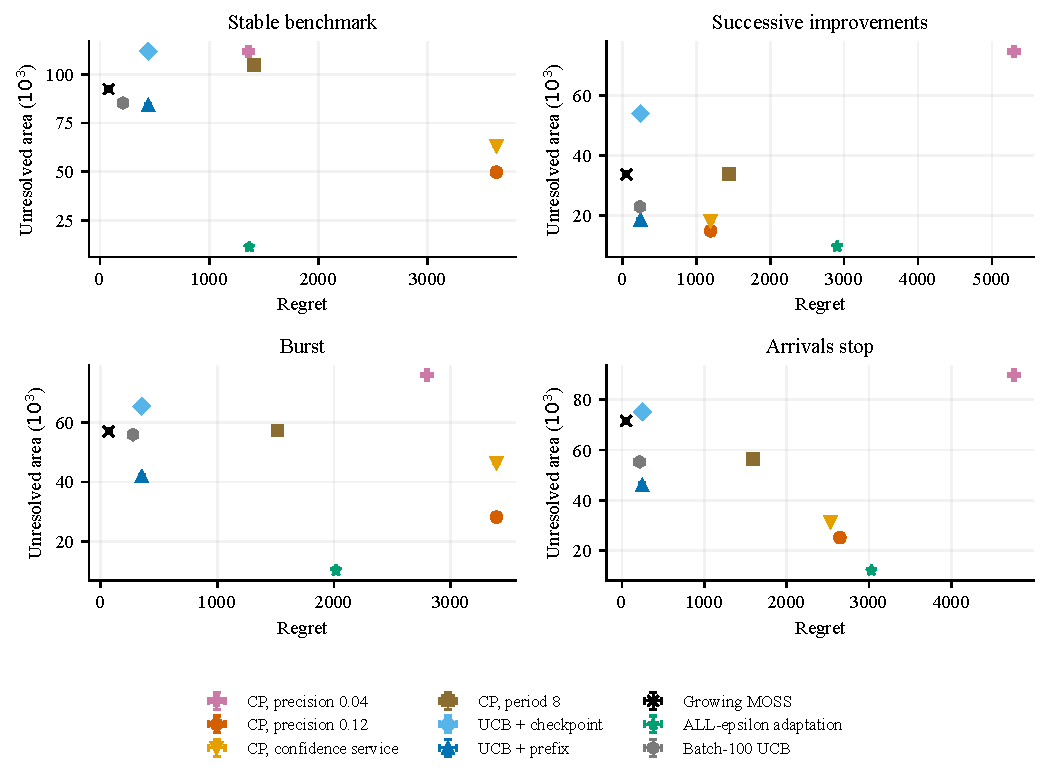
\includegraphics[width=.97\textwidth]{figures/fig_cost_area.pdf}
\caption{Regret and cumulative $\eta$-unresolved area for all nine methods.
Lower values on both axes are preferable. CP denotes the Checkpoint-UCB
configurations described in the text. Error bars quantify Monte Carlo
uncertainty. Neither checkpoint precision nor its allocation variants
uniformly dominate the confidence-based adaptation.}
\label{fig:cost-area}
\label{fig:legacy-costs}
\end{figure}

\subsection{Finite-budget findings and their limits}

In all 640 finer-checkpoint runs, every available arm remains unresolved
at every time step. Five to eight arms contribute to the final
$\eta$-unresolved count because the metric exempts the boundary band;
the remaining arms have not been classified. Its zero-error record
therefore does not establish useful classification at this budget.
The charged unresolved area ranges from 74,820 to 111,784. This is a
limitation of the conservative construction at the chosen budget.
The confidence-based adaptation resolves every $\eta$-separated arm by
the endpoint in all replications of these four environments.

The coarser checkpoints reduce area relative to UCB alone, but can incur
much larger regret. Under the stable benchmark, CP-FIFO has mean regret
3629.9 and area 49,718, compared with 1367.8 and 11,306 for
ALL-$\varepsilon$ adaptation. The paired differences, CP-FIFO minus the
adaptation, are $2262.1$ (standard error $11.7$) for regret and
$38{,}411.7$ (standard error $241.9$) for area. The adaptation improves
both quantities in the burst environment as well. These findings do not
support a general numerical advantage of checkpoint FIFO over a strong
history-retaining identification rule.

Under successive improvements, CP-FIFO occupies a different cost point:
regret 1194.7 and area 14,743, compared with 2905.8 and 9525 for the
adaptation. The paired regret difference is $-1711.0$ (standard error
$2.4$), and the area difference is $5217.7$ (standard error $141.1$).
This comparison does not isolate task expiration. The adaptation uses
all 10,000 designated service pulls, whereas coarse CP uses about 5,786;
some remaining questions fall inside the unpenalized boundary band.
The regret difference can therefore partly reflect different stopping
rules for reporting work. Identifying the mechanism requires a comparison
with the same boundary tolerance and service requirement. These observed
cost points do not estimate an optimal frontier.

Growing-MOSS has the smallest mean regret in all four environments,
between 52.0 and 77.3, while leaving substantially larger unresolved
areas. Small regret alone provides little evidence of timely set
maintenance; it does not rule out adding an effective certification
layer to that allocation rule. Explicit service pays for observations of
inferior arms. Reducing service from every second to every eighth pull
generally reduces regret and enlarges unresolved area. Confidence-driven
checkpoint service does not uniformly improve either criterion.

\begin{figure}[t]
\centering
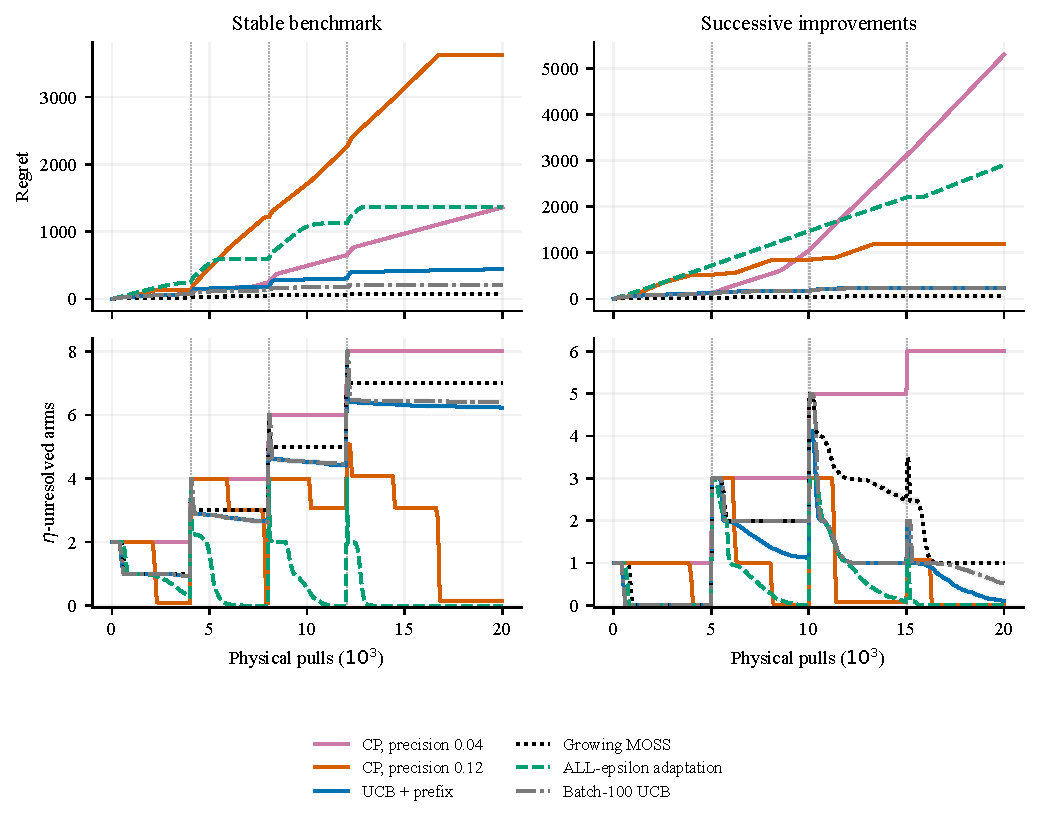
\includegraphics[width=.98\textwidth]{figures/fig_paths_pair1.pdf}
\caption{Mean regret and mean $\eta$-unresolved arm counts at the physical
sampling clock. Bands are 1.96 Monte Carlo standard errors; vertical dotted
lines mark arrivals. Stable and improving benchmarks are shown here,
with the other two environments in Appendix~\ref{app:computation}.
The six methods in Table~\ref{tab:simulation} are displayed. The saved results retain all
nine methods and their paths on the common observation grid.}
\label{fig:paths}
\label{fig:legacy-paths}
\end{figure}

For Batch100-UCB, the admission-delay contributions to regret are $0$,
$33.92$, $16.00$, and $22.40$ in the four environments. No historical
retirement deficit occurred in these runs. Appendix~\ref{app:computation}
defines this decomposition and distinguishes it from learning within the
reward-active set.

There were no incorrect positive or negative reports in any of the 5,760
runs. For one fixed method and environment, zero failures in 160
replications gives an exact one-sided 95\% upper confidence bound below
0.0186 on its failure probability. This finite experiment does not
establish uniform reliability over all environments and times. Nor do
the eight-arm comparisons validate the asymptotic lower bounds, settle
the critical logarithmic gap, or establish checkpoint optimality.
They quantify the finite-budget cost of the conservative quotas and
show why reward and maintenance must be reported together.

\subsection{Configuration, records, and implementation names}
\label{app:computation}

This earlier numerical study has four environments, nine methods, and 160 paired
replications per environment, for 5,760 runs of 20,000 physical pulls.
The six methods in Table~\ref{tab:simulation} appear in both path
figures. The cost--area figure and Table~\ref{tab:allocation} include all nine.

The local reproducibility materials contain the complete configuration,
run-level records, saved paths, summary statistics, and paired differences
in \texttt{experiments/results/}. The configuration gives every arrival
time and mean, each method's parameters, and the seed mechanism. For
replication seed $s$ in environment index $j$, the generator is NumPy
PCG64 initialized with \texttt{SeedSequence([s,j])}, where
$s=202610150,\ldots,202610309$ and $j=0,\ldots,3$.
The resulting Bernoulli potential streams are shared across methods.
The policy uses only observed rewards and current arrivals. Array
preallocation is simulation storage and does not expose future arms or
the evaluation endpoint to a policy.

The reporting configuration is named Checkpoint-UCB in the article.
For reproducibility, its unchanged reference interface is
\texttt{CheckpointUCBAA} in \texttt{reference\_cp\_ucb\_aa.py}.
The experiment driver is \texttt{run\_experiments.py}.
The data IDs \texttt{CP-FIFO-fine}, \texttt{CP-FIFO},
\texttt{CP-confidence}, and \texttt{CP-period8} retain their existing
meaning. In particular, the first two are FIFO service every second pull
with $\rho=.04$ and $.12$; the latter two change allocation as specified
in this section. The remaining IDs are \texttt{UCB-checkpoint},
\texttt{UCB-prefix}, \texttt{Growing-MOSS},
\texttt{ALL-epsilon-adapt}, and \texttt{Batch100-UCB}.
The ALL-$\varepsilon$ rule is a specified retained-history adaptation,
not a reproduction of FAREAST or $(\mathrm{ST})^2$.

\texttt{runs.csv} records one row per environment, seed, and method,
including full-run label errors, both unresolved-area totals, service
counts and regret, final per-arm counts, and the regret components below.
\texttt{paths.npz} contains all nine methods' regret, unresolved counts,
cumulative area, and total unresolved counts on a common grid, with
every arrival included. This is a saved time grid, not a per-round action
log. \texttt{summary.csv} and \texttt{paired\_differences.csv} provide
the numerical summaries; the two table source files are generated from
these records. \texttt{figures/gen\_fig\_performance.py} is the plotting
and tabulation entry point.

\begin{table}[t]
\centering
\caption{Allocation diagnostics. Each cell gives mean forced service pulls and mean final $\eta$-unresolved arms. UCB and MOSS have zero forced service.}
\label{tab:allocation}
\small
\begin{tabular}{lrrrr}
\toprule
Method & Stable & Improvements & Burst & Stop \\
\midrule
CP-FIFO ($\rho=.04$) & 10000, 8.00 & 10000, 6.00 & 10000, 5.00 & 10000, 5.00 \\
CP-FIFO ($\rho=.12$) & 7340, 0.16 & 5786, 0.00 & 5991, 0.00 & 5737, 0.00 \\
CP-confidence & 7144, 0.16 & 4653, 0.00 & 6092, 0.00 & 5322, 0.00 \\
CP-period8 & 2500, 6.74 & 2500, 0.20 & 2225, 3.00 & 2500, 2.00 \\
UCB-checkpoint & 0, 8.00 & 0, 3.00 & 0, 4.00 & 0, 4.00 \\
UCB-prefix & 0, 6.23 & 0, 0.11 & 0, 1.69 & 0, 1.71 \\
Growing-MOSS & 0, 7.00 & 0, 1.00 & 0, 4.00 & 0, 4.00 \\
ALL-$\varepsilon$ adapt. & 3696, 0.00 & 10000, 0.00 & 7794, 0.00 & 10000, 0.00 \\
Batch100-UCB & 0, 6.40 & 0, 0.53 & 0, 4.00 & 0, 2.89 \\
\bottomrule
\end{tabular}
\end{table}


\begin{figure}[p]
\centering
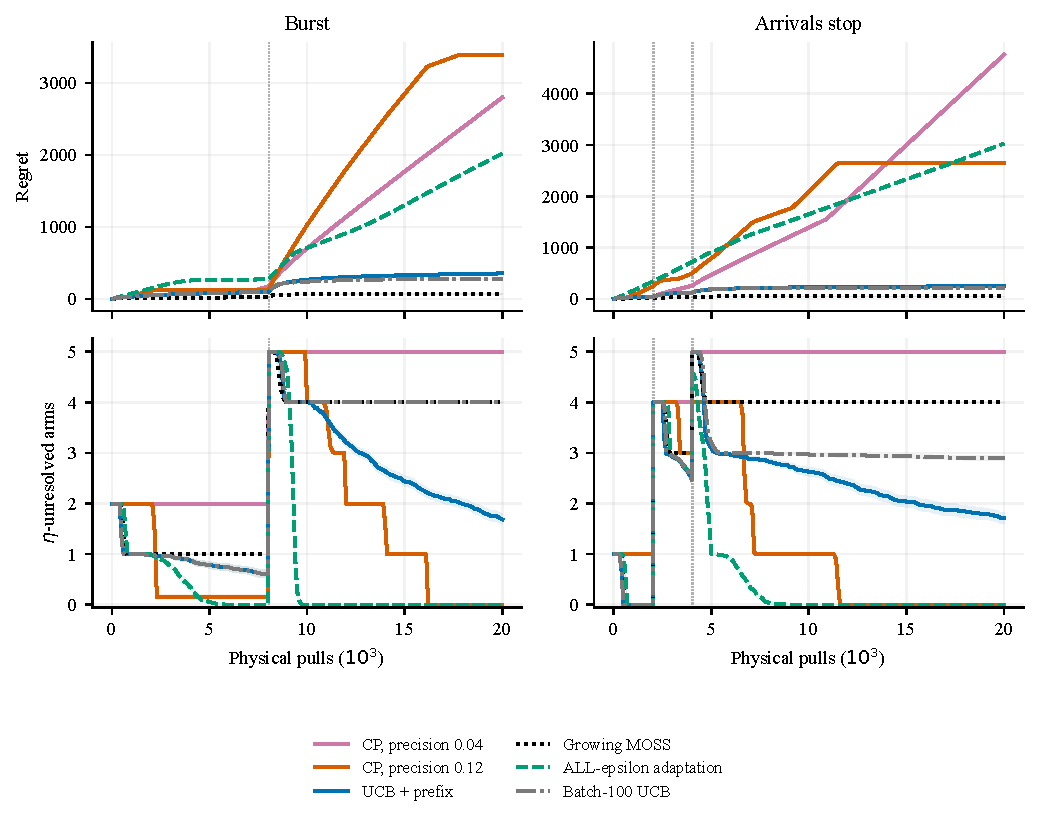
\includegraphics[width=.98\textwidth]{figures/fig_paths_pair2.pdf}
\caption{Additional paths for the burst and stopped-arrival environments.
The six displayed policies, common potential reward streams, 160
replications, and 1.96 Monte Carlo standard error bands are the same as
in Figure~\ref{fig:paths}. Vertical lines mark actual arrivals. The full
run-level data and saved paths retain all nine policies.}
\label{fig:paths-additional}
\end{figure}

\subsection{Admission and reward-retirement accounting}

Let $\mathcal A_t^{\rm adm}\subseteq\mathcal A_t$ be the arms admitted
for reward selection, and let $B_t\subseteq\mathcal A_t^{\rm adm}$ be
its nonempty reward-active subset. Assume $I_t\in B_t$. Adding and
subtracting the admitted and active best means at each physical pull gives
the pathwise identity
\begin{equation}
\begin{aligned}
R_T={}&\sum_{t\le T}\bigl(\max_{i\in B_t}r_i-r_{I_t}\bigr)\\
&+\sum_{t\le T}\bigl(r^*(t)-\max_{i\in\mathcal A_t^{\rm adm}}r_i\bigr)
+\sum_{t\le T}\bigl(\max_{i\in\mathcal A_t^{\rm adm}}r_i
                         -\max_{i\in B_t}r_i\bigr).
\end{aligned}
\label{eq:three_part}
\end{equation}
The components are within-active learning, admission delay, and the
historical-retirement deficit. They are all nonnegative. In Batch100-UCB,
admission occurs at pulls $1,101,201,\ldots$, before action selection.
Reward retirement uses the confidence comparison among currently
admitted active arms after the current observation. Reporting continues
to cover all physically arrived arms, with $[0,1]$ intervals before
admission. Neither waiting for admission nor reward retirement is itself
a certificate of membership or nonmembership in the near-optimal set.

For Checkpoint-UCB, every arrived arm is immediately reward-eligible,
and negative reporting does not remove it from reward selection.
Thus $B_t=\mathcal A_t^{\rm adm}=\mathcal A_t$, so the last two
components vanish identically. The same statement applies to the other
immediate-admission methods that retain every arm for reward selection.

In the Batch100-UCB records, the admission contributions are $0$, $33.92$,
$16.00$, and $22.40$ for the stable, improving, burst, and stopped-arrival
environments, respectively. No retirement deficit occurred. Across all
5,760 records, the largest absolute difference between regret and the
sum in \eqref{eq:three_part} is below $3.1\times10^{-12}$.

\subsection{Verification and computational resources}

The production manifest records Python 3.11.7, NumPy 1.26.4, Numba 0.59.0,
Windows 10, and 13.5 seconds for production generation and recording,
excluding initial compilation and subsequent plotting. The resource snapshot records
20 physical CPU cores, 28 logical cores, and 31.71 GB system memory.
The small physical-round loops use compiled CPU execution. A detected GPU
was not needed. Dependencies and hashes of the reference implementation,
driver, configuration, and numerical records accompany the materials.

The saved production parity check compared the compiled FIFO procedure
with the reference interface for 20,000 consecutive rounds, checking
actions, service indicators, available-arm counts, and reports. That is a
historical implementation check. During the first revision, separate short
deterministic checks compare the same interfaces around arrivals, quota
crossings, frozen intervals, and negative reports. That revision also
recomputed the 24 legacy-table rows, the complete allocation table, and the
640 all-unresolved finer-checkpoint records from the saved data.
These operations leave the simulation records and policy code unchanged.
They are implementation and accounting checks, rather than new method
comparisons or probability certificates.

The local materials support these resource and reproducibility
descriptions. A public repository or permanent release identifier has not
been verified for this version.



\subsection{Historical all-prefix report}
\label{app:legacy-prefix}
The all-prefix reporter in this earlier comparison uses the following
Hoeffding intervals. These are separate from F-CCP's mixed evidence and
its persistent reporting-failure rule.
With
\[
 b_i(n)=\sqrt{\frac{\log(8i^2n^2/\delta)}{2n}},
\]
the union of all potential-prefix failures has probability at most
$\delta\zeta(2)^2/4<\delta$. Intersecting the prefix intervals with $[0,1]$
therefore gives simultaneous coverage. On that event each endpoint differs
from its mean by at most $2b_i(n)$. No conditioning on a previously selected
empirical mean is used. Empty intersections on failure paths are handled by
exclusion-first reporting; the reward policy remains defined on all paths.


\FloatBarrier

% END MERGED SUPPLEMENTARY MATERIAL
\FloatBarrier
\bibliographystyle{plainnat}
\bibliography{references}
\end{document}
